% Master's thesis, Departamento de Informática, Universidad Técnica Federico Santa María.
% Based on the DI/UTFSM thesis template by Daniel San Martín Reyes.
\documentclass[12pt, letterpaper]{book}

%%% PACKAGES %%%
\usepackage[utf8]{inputenc}
\usepackage[margin=1.1in]{geometry}
\usepackage{amsfonts}
\usepackage{amssymb}
\usepackage{amsmath}
\usepackage{graphicx}
\usepackage{subcaption}
\usepackage{hyperref}
\usepackage{tabularx}
\usepackage{booktabs}
\usepackage{color}
\usepackage{url}
\usepackage{multirow}
\usepackage{mathtools}
\usepackage{tablefootnote}
\usepackage{fancyhdr}
\usepackage{longtable}
\usepackage{pdfpages}
\usepackage{siunitx}
\usepackage{gensymb}
\usepackage{physics}
\usepackage[nosectionbib]{apacite}
\usepackage{notoccite}
\usepackage{placeins}
\usepackage{pdflscape}
\usepackage{tikz}
\usetikzlibrary{arrows.meta}

% Float placement
\renewcommand{\topfraction}{0.85}
\renewcommand{\bottomfraction}{0.70}
\renewcommand{\textfraction}{0.12}
\renewcommand{\floatpagefraction}{0.75}
\setcounter{topnumber}{3}
\setcounter{bottomnumber}{2}
\setcounter{totalnumber}{4}

\raggedbottom

% Citation years in dark red
\definecolor{darkred}{RGB}{139,0,0}
\makeatletter
\let\oldAPACyear\APACyear
\renewcommand{\APACyear}[1]{\textcolor{darkred}{\oldAPACyear{#1}}}
\makeatother

%%% SETUP %%%

% Hyperref %
\hypersetup{
    hidelinks,
    linktoc=section,
}

% Bibtex %
\bibliographystyle{apacite}


% Definitions %
% Text
\providecommand{\keywords}[1]{\textbf{\textit{Keywords}}: #1.}
\providecommand{\eskeywords}[1]{\textbf{\textit{Palabras clave}}: #1.}

\usepackage[usenames]{xcolor}
\definecolor{color_morado}{HTML}{9B59B6}
\def\purple#1{\textcolor{color_morado}{#1}}


\pagestyle{fancy}
\fancyhf{}% Clear page header/footer
\fancyhead[RO, LE]{\leftmark}
\fancyfoot[C]{\thepage}

%Hyphen
% \hyphenation{} % Add words to hyphenate if needed


\begin{document}

    % Front %
    %\maketitle
    \begin{titlepage}
	\centering
	{\large UNIVERSIDAD TÉCNICA FEDERICO SANTA MARÍA \par}
	{\normalsize DEPARTAMENTO DE INFORMÁTICA \par}
	{\normalsize VALPARAÍSO - CHILE \par}
	\vspace{1cm}
	
\includegraphics[width=.3\textwidth]{figures/logos/utfsm.pdf}\par
	\vspace{2cm}
	{\Large\bfseries Deep learning for extensive air showers reconstruction: an interpretable multi-task CNN-Transformer model for the CONDOR observatory \par}
	\vspace{2cm}
	{\large Luis Felipe Navarro Farías \par}
	\vspace{2cm}
    {\small Thesis presented in partial fulfillment of the requirements for the degree of\\
        Magíster en Ciencias de la Ingeniería Informática \par}
    \vspace{3cm}
    {\small
        Advisor: Raquel Pezoa, Ph.D.\\
        Co-Advisor: Nicolás Viaux, Ph.D.\\
        \textcolor{red}{[TODO]}
    }
	\vfill
	{\normalsize \textcolor{red}{[TODO: fecha de defensa]} \par}
\end{titlepage}

    
    % Committee %
    \thispagestyle{empty}
{\setlength{\parindent}{0cm}
    {\normalsize \uppercase{Thesis Title}: \par}
    \vspace{.5cm}
    {\normalsize \bfseries Deep learning for extensive air showers reconstruction: an interpretable multi-task
    CNN-Transformer model for the CONDOR observatory \par}
    \vspace{2cm}
    {\normalsize \uppercase{Author:} \par}
    \vspace{.5cm}
    {\normalsize\bfseries Luis Felipe Navarro Farías \par}
    \vspace{2cm}
    {\normalsize Thesis presented in partial fulfillment of the requirements for the degree of Magíster en Ciencias de la Ingeniería Informática  of the Universidad Técnica Federico Santa María.\par}
    \vspace{2cm}
    {\normalsize Raquel Pezoa, Ph.D. \hfill \raisebox{-\baselineskip}{\shortstack{\underline{\hspace{10cm}}\\Advisor}} \par}
    \vspace{1cm}
    {\normalsize Nicolás Viaux, Ph.D. \hfill \raisebox{-\baselineskip}{\shortstack{\underline{\hspace{10cm}}\\Co-Advisor}} \par}
    \vspace{1cm}
    {\normalsize \textcolor{red}{[TODO]} \hfill \raisebox{-\baselineskip}{\shortstack{\underline{\hspace{10cm}}\\~}} \par}
    \vspace{1cm}
    {\normalsize \textcolor{red}{[TODO]} \hfill \raisebox{-\baselineskip}{\shortstack{\underline{\hspace{10cm}}\\~}} \par}
    
    
    \vfill
    
    \raggedleft
    {\small Valparaíso, Chile. \par}
    {\small \today. \par}
}

    
    % USM format margin
    \newgeometry{top=.9in, bottom=.9in, left=4cm, right=2.5cm, headheight=15pt, headsep=0.2in, includehead}
    
    \pagenumbering{Roman} % Roman numbering for toc
    
    % Dedicatory
    \thispagestyle{empty}

\vspace*{18cm}

\begin{flushright}
    To my beloved Liza, my parents,\\
    and my dear little cat Thorfinn
\end{flushright}


    \let\cleardoublepage\clearpage
    
    % Acknowledgements
    \chapter*{Acknowledgments}
\linespread{1.12}\selectfont

A la profesora {\bfseries\color{darkred}Raquel Pezoa}, quien me ha guiado y
ayudado con absolutamente todo, desde mi licenciatura en física hasta esta tesis.
Nada de esta investigación existiría sin su acompañamiento; su disposición es
admirable y la llevaré siempre conmigo.

Al profesor {\bfseries\color{darkred}Nicolás Viaux}, por guiarme desde el lado
más teórico con ideas y consejos que enriquecieron este trabajo.

A {\bfseries\color{darkred}Liza}, mi gran compañera de vida, que siempre me ha
apoyado, comprendido y levantado, sin importar la situación. Es mi inspiración
para ser mejor persona, mejor investigador y alguien completamente feliz. La
admiro y la amo desde lo más profundo de mi corazón.

A {\bfseries\color{darkred}Yerko} y {\bfseries\color{darkred}Daniel},
compañeros de física desde los inicios y mis dos pokémon starters, por su
sabiduría y compañerismo durante toda esta travesía. A mis amigos de toda la
vida ---{\bfseries\color{darkred}Naxo}, {\bfseries\color{darkred}Nico},
{\bfseries\color{darkred}Julito}, {\bfseries\color{darkred}Tatis},
{\bfseries\color{darkred}Maury} y {\bfseries\color{darkred}Claudia}---, que
forjaron quién soy y llenan de alegría mi vida.

A mis padres, {\bfseries\color{darkred}Marcelo} y
{\bfseries\color{darkred}Ximena}, a quienes amo con todo mi corazón y estaré
agradecido de por vida: son el pilar que me permitió llegar hasta donde estoy y
ser quien soy. A mis hermanos, {\bfseries\color{darkred}Nicolás},
{\bfseries\color{darkred}Marcelo} y {\bfseries\color{darkred}Jesús}, personas
inteligentísimas que, cada uno a su manera, han nutrido mi conocimiento
profesional y de la vida.

Finalmente, a mi gatito {\bfseries\color{darkred}Thorfinn}, que sin hablar me
consuela, con un maullido alegra mi día entero y demuestra su amor con rasguños
y ganas de comer. Me espera cada día e hizo que mis días nunca más fuesen
solitarios; me demostró que no se necesitan palabras para querer.

% Separator
\begin{center}
\begin{tikzpicture}[baseline=-0.5ex]
  \draw[darkred, line width=0.4pt] (-3.2,0) -- (-0.22,0);
  \draw[darkred, line width=0.4pt] (0.22,0) -- (3.2,0);
  \fill[darkred] (0,0.09) -- (0.09,0) -- (0,-0.09) -- (-0.09,0) -- cycle;
  \fill[darkred] (-0.17,0) circle (0.02);
  \fill[darkred] (0.17,0) circle (0.02);
\end{tikzpicture}
\end{center}

{\linespread{1.0}\selectfont\small This work was supported by ANID CCTVal (CIA250027) and by Proyectos Internos de Investigación USM 2025 (PI\_LII\_25\_06). The author also acknowledges the support of the Becas Magíster Científico-Tecnológico of the Universidad Técnica Federico Santa María.\par}

    \let\cleardoublepage\clearpage
    
    %Abstract
    \chapter*{Resumen}

La reconstrucción de duchas atmosféricas extensas (extensive air showers, EAS) en el régimen sub-TeV es un desafío central para los observatorios de astropartículas de gran altitud. En este trabajo desarrollamos y evaluamos un método de aprendizaje profundo multitarea que reconstruye simultáneamente tres propiedades de las EAS --- discriminación gamma-hadrón, ángulo cenital y energía primaria --- en el observatorio CONDOR (Desierto de Atacama, Chile, 5.300~m s.n.m.). El modelo es una arquitectura híbrida CNN--Transformer con dos streams de atención por tarea: uno sobre las características procesadas por la CNN y otro directamente sobre la secuencia cruda de hits.
%
Entrenado con datos simulados por CORSIKA en el rango 300--800~GeV, el modelo alcanza un AUC de 0{,}991 y un F1-score de 0{,}970 en la discriminación gamma-hadrón, un error angular medio de $0{,}484\degree$ en el ángulo cenital y un error absoluto medio de $103{,}72~\mathrm{GeV}$ en la energía. La importancia de características por permutación (PFI) y el análisis de ablación coinciden en que la información temporal domina la reconstrucción angular, mientras que las características espaciales y de energía depositada gobiernan la clasificación. La atención sobre la secuencia cruda muestra que cada tarea pondera una parte distinta de la secuencia: la clasificación, su borde inicial; la reconstrucción angular, su parte tardía.
%
Un estudio de dropout de detectores muestra que la discriminación gamma-hadrón es la tarea más tolerante a fallos, y que un núcleo denso favorece la clasificación y el ángulo, mientras que la energía requiere cobertura lateral; la optimización del \textit{layout} queda como trabajo futuro. Estos resultados muestran que el aprendizaje multitarea con explicabilidad integrada es un enfoque viable para la reconstrucción de EAS en observatorios de próxima generación.

\bigskip

\eskeywords{Rayos cósmicos, rayos gamma, duchas atmosféricas extensas, aprendizaje profundo, redes neuronales convolucionales, transformers, aprendizaje multitarea, inteligencia artificial explicable, mecanismos de atención}


    \addcontentsline{toc}{chapter}{Resumen}
    \let\cleardoublepage\clearpage
    
    \chapter*{Abstract}

The reconstruction of extensive air showers (EAS) in the sub-TeV regime is a central challenge for high-altitude astroparticle observatories. In this work, we develop and evaluate a multi-task deep learning method that simultaneously reconstructs three EAS properties --- gamma-hadron discrimination, zenith angle, and primary energy --- at the CONDOR Observatory (Atacama Desert, Chile, 5,300~m a.s.l.). The model is a hybrid CNN--Transformer architecture with two attention streams per task: one on CNN-processed features and one directly on the raw hit sequence.
%
Trained on CORSIKA-simulated events in the 300--800~GeV range, the model achieves an AUC of 0.991 and an F1-score of 0.970 for gamma-hadron discrimination, a mean angular error of $0.484\degree$ for the zenith angle, and a mean absolute error of $103.72~\mathrm{GeV}$ for the energy. Permutation feature importance (PFI) and feature ablation agree that temporal information dominates angular reconstruction, while spatial and deposited-energy features govern classification. Attention on the raw sequence shows that each task weights a different part of the sequence: classification, its leading edge; angular reconstruction, its late portion.
%
A detector dropout study shows that gamma-hadron discrimination is the most fault-tolerant task, and that a dense core favours classification and angular reconstruction, while energy needs lateral coverage; a full layout optimisation is left for future work. These results show that multi-task learning with integrated explainability is a viable approach to EAS reconstruction in next-generation astroparticle observatories.

    \bigskip

    \keywords{Cosmic ray, gamma ray, extensive air showers, deep learning, convolutional neural networks, transformers, multi-task learning, explainable artificial intelligence, attention mechanisms}

    \addcontentsline{toc}{chapter}{Abstract}
    
    % General Index
    \tableofcontents
    \addcontentsline{toc}{chapter}{Contents}
    \let\cleardoublepage\clearpage
    
    % List of Figures %
    \listoffigures
    \addcontentsline{toc}{chapter}{List of Figures}
    \let\cleardoublepage\clearpage
    
    % List of Tables %
    \listoftables
    \addcontentsline{toc}{chapter}{List of Tables}
    \let\cleardoublepage\clearpage
    
    \clearpage
    
    \pagenumbering{arabic} % Arabic numbering for chapters
    
    
    %%% CHAPTERS %%%

    % Chapter 1: Introduction %
    \chapter{Introduction} \label{ch:introduction}

The universe is permeated by a continuous flux of high-energy particles arriving at Earth from all directions. These particles, recognized as cosmic rays, were first identified in the early twentieth century~\shortcite{hess1912beobachtungen} and remain an active area of astrophysical research~\shortcite{bell2013cosmic}. Despite significant experimental progress, the precise locations of their astrophysical sources, as well as the physical mechanisms governing their acceleration to ultra-high energies, have not yet been definitively established~\shortcite{blasi2013origin}. Understanding cosmic rays provides an observational window into some of the most energetic and extreme environments in the universe.

\section{From Cosmic Rays to the CONDOR Observatory}

A central goal of high-energy astrophysics is identifying the acceleration sites of cosmic rays. Because cosmic rays are predominantly charged particles, their trajectories are deflected by galactic magnetic fields, erasing any directional information about their sources by the time they arrive at Earth. Gamma rays, being electrically neutral, travel in straight lines from their production sites and therefore serve as direct tracers of cosmic ray activity~\shortcite{morrison1958gamma}. However, isolating these photon signals from the overwhelming background of hadronic cosmic ray events constitutes a central challenge for ground-based observatories~\shortcite{alfaro2022gamma, deligny2025searches, schneider2026deep}. The physics underlying this challenge is discussed in detail in Chapter~\ref{ch:theo-back}.

When a high-energy primary particle strikes the upper atmosphere, it initiates a multiplying cascade of secondary particles known as an extensive air shower (EAS)~\shortcite{rao1998extensive}. The secondary particles that survive to the detector level form a spatiotemporal footprint across the array. Reconstructing the primary particle's type, energy, and arrival direction from this sparse and stochastic footprint is the central problem of ground-based astroparticle physics and of this thesis.

An observational gap exists in the sub-TeV window between 100 GeV and 1 TeV: space-based instruments such as the Fermi Large Area Telescope (Fermi-LAT) are limited by collection area at higher energies~\shortcite{ackermann2012fermi}, while ground-based installations at altitudes around 4,000 m impose effective energy thresholds\footnote{The \textit{effective energy threshold} is the lowest primary energy at which an array can still detect and reconstruct showers with reasonable efficiency. It is set by how much of the shower survives down to the observation altitude, and is discussed further in Chapter~\ref{ch:theo-back}.} of several hundred GeV. The CONDOR observatory~\shortcite{arratia2025condor}, planned for Cerro Toco in the Atacama Astronomical Park at 5,300 m above sea level, is designed to bridge this gap by intercepting the shower front closer to its atmospheric maximum, lowering the effective energy threshold to approximately 100 GeV.

Analyzing the low-energy events accessible to CONDOR presents a significant computational challenge. At 100 GeV, the spatiotemporal footprint of a shower is sparse, noisy, and subject to large stochastic fluctuations, and extracting the kinematic properties of the primary particle from it is an inverse problem with no closed-form solution.

\section{Deep Learning and Explainability}

Historically, EAS observatories relied on classical parametric algorithms, for example, planar fitting for arrival direction reconstruction~\shortcite{pierre2014reconstruction} and the Nishimura-Kamata-Greisen lateral distribution function~\shortcite{nishimura1958kamata} for energy estimation~\shortcite{kawata2017energy}. While computationally lightweight, these methods show degraded performance under the noise conditions and sparse hit patterns of low-energy showers, and they cannot naturally handle the simultaneous estimation of multiple shower properties.

Deep learning~\shortcite{lecun2015deep} shifts this paradigm by enabling end-to-end representation learning directly from raw detector hits. Convolutional neural networks (CNNs)~\shortcite{lecun1998convolutional} have proven effective at extracting local features from the hit patterns of dense detector arrays~\shortcite{okukawa2024neural}, while Transformer architectures~\shortcite{vaswani2017attention}, through their self-attention mechanism, are well suited for capturing the global, long-range correlations that span the full shower footprint~\shortcite{lin2022survey, langner2024deep}. Despite recent advances, existing frameworks for EAS reconstruction often constrain themselves to single-task objectives or rely on detector geometries dissimilar to CONDOR~\shortcite{erdmann2018deep, okukawa2024neural}, making direct translation difficult. The predecessor to this work~\shortcite{navarro2025multi} introduced a CNN-LSTM architecture for CONDOR that addressed two of the three tasks --- particle classification and zenith angle regression --- but remained limited by sequential processing constraints and the absence of energy estimation as a third reconstruction task. This thesis extends that foundation with a hybrid CNN-Transformer architecture capable of simultaneously addressing gamma-hadron discrimination, zenith angle reconstruction, and primary energy estimation within a unified multi-task framework.

An ongoing challenge in the scientific adoption of deep learning is the tension between predictive performance and physical interpretability~\shortcite{ribeiro2016should}. A model achieving high reconstruction accuracy yields limited scientific value if its predictions rely on non-physical or spurious correlations in the training data. This concern is particularly relevant when the model is trained on data synthesized by a Monte Carlo framework like CORSIKA~\shortcite{Heck1998}, the standard simulation code for extensive air showers, which is described in detail in Section~\ref{sec:corsika}; under these conditions, the risk of learning simulation artifacts rather than genuine shower physics cannot be dismissed without explicit verification. This is why the adoption of explainable artificial intelligence (XAI) methods~\shortcite{adadi2018peeking} is indispensable for understanding the model’s reasoning when generating predictions.

This thesis addresses this requirement through two complementary feature importance methods --- permutation feature importance~\shortcite{altmann2010permutation} and a feature ablation study, which quantify the contribution of each input channel to each reconstruction task by intervening on the input --- together with an analysis of the attention patterns, which describes the temporal focus of the Transformer streams along the shower front. Confirming that these analyses align with physical expectations constitutes a key scientific deliverable of this work, alongside the reconstruction performance itself.

\section{Objectives}

The primary objective of this thesis is to design, evaluate, and interpret a deep learning model for the simultaneous reconstruction of multiple physical properties of extensive air showers, specifically developed for the high-altitude conditions of the CONDOR observatory.

The specific objectives are:
\begin{enumerate}
    \item \textbf{To design} and implement a hybrid CNN-Transformer multi-task architecture capable of simultaneously performing gamma-hadron discrimination, zenith angle regression, and primary energy estimation from variable-length sequences of spatiotemporal detector hits.
    
    \item \textbf{To devise} a data preprocessing and stratified balancing strategy that mitigates the class and configuration imbalances inherent in Monte Carlo simulation datasets.
    
    \item \textbf{To evaluate} the architecture's performance on a held-out test set and compare its reconstruction accuracy against classical baselines and prior deep learning approaches for CONDOR.
    
    \item \textbf{To interpret} the learned representations using permutation feature importance, feature ablation, and attention pattern analysis, validating their physical consistency against established shower phenomenology.
    
    \item \textbf{To identify} the structural and algorithmic limitations of the current framework and provide a transparent methodological foundation for future adaptation to real detector data once CONDOR begins operations.
\end{enumerate}

\section{Contributions Beyond the Published Work}
\label{sec:contributions_intro}

The core multi-task reconstruction results and the three-stream CNN-Transformer architecture have been published in a companion paper in \emph{Astronomy and Computing}~\shortcite{navarro2026transformer}. This thesis extends that published work in several directions that are not covered by the paper:
\begin{itemize}
    \item An extended six-stream architecture with independent RAW attention streams per task, enabling hit-level interpretability without convolutional indirection.
    \item A feature ablation study as a second, independent method for validating feature importance, complementing the permutation-based analysis reported in the paper.
    \item A ROC analysis grouped by primary energy and zenith angle, revealing the physically consistent energy dependence of discrimination performance.
    \item A detector robustness study quantifying the fault tolerance of the trained model to missing detectors across the three tasks.
\end{itemize}

\section{Thesis Structure}

The remainder of this thesis is organized as follows. Chapter~\ref{ch:theo-back} establishes the theoretical foundations of the work, covering the physics of cosmic rays and extensive air showers, the CONDOR observatory and its simulation framework, and the deep learning architectures and explainability methods employed. Chapter~\ref{ch:methodology} describes the full methodological pipeline, from dataset construction and preprocessing through model architecture, hyperparameter optimization, and training configuration. Chapter~\ref{ch:results} presents the results across all three reconstruction tasks and the explainability analysis. Chapter~\ref{ch:conclusions} concludes with a summary of the main findings, a discussion of limitations, and directions for future work.
    
    % Chapter 2: Theoretical Background %
    \chapter{Theoretical Background} \label{ch:theo-back}

This chapter establishes the physical and computational foundations necessary for the reconstruction of EAS at CONDOR. The chapter begins with the properties and astrophysical context of cosmic rays, followed by the phenomenology of atmospheric particle cascades and the principles of ground-based detection. It then describes the CONDOR observatory and the Monte Carlo simulation framework used to generate the training data. Finally, it introduces the deep learning architectures and explainability methods that form the technical core of this thesis.

\section{Cosmic Rays and High-Energy Astrophysics}

The study of cosmic rays sits at the intersection of particle physics, astrophysics, and cosmology. First discovered in 1912 by Victor Hess~\shortcite{hess1912beobachtungen} through a series of balloon ascents that measured increasing ionization rates with altitude, cosmic rays are not electromagnetic radiation but high-energy subatomic particles, primarily bare atomic nuclei, traveling through space at relativistic speeds~\shortcite{longair2011high}. They carry information about some of the most extreme physical environments in the universe, yet the precise mechanisms behind their acceleration remain one of the central open problems in modern astrophysics~\shortcite{blasi2013origin}.

Decades of space-based and balloon-borne measurements have established a precise picture of the composition of cosmic rays at sub-TeV energies. By particle flux, approximately 89\% of primary cosmic rays are protons, roughly 10\% are helium nuclei, and the remaining fraction consists of heavier atomic nuclei up to iron, alongside electrons, positrons, and traces of antimatter~\shortcite{ParticleDataGroup2024}.

Because these primaries are electrically charged, their propagation through the interstellar and intergalactic medium is governed by the Lorentz force, which continuously deflects their trajectories as they pass through irregular galactic magnetic fields. Over astronomical distances, this deflection randomizes their arrival directions at Earth, permanently erasing the geometric line of sight between their production sites and the observer. As a consequence, identifying cosmic ray sources through arrival direction alone is not generally possible, and indirect tracers such as gamma rays and neutrinos become essential tools.

\subsection{The Energy Spectrum}

The energy spectrum of cosmic rays spans more than twelve orders of magnitude and follows a sequence of power laws of the form 
\begin{equation}
  \Phi(E) \propto E^{-\gamma}  
\end{equation}
where $\Phi(E)$ is the differential flux and $\gamma$ is the spectral index. Rather than a single unbroken power law, the spectrum exhibits well-characterized structural breaks that reflect transitions between different source populations, acceleration limits, and propagation regimes. For example, as illustrated in Figure~\ref{fig:crs-spectrum}, precise measurements of this spectrum reveal distinct steepenings and flattenings at specific energy scales — commonly referred to as the \textit{knee}, the \textit{second knee}, and the \textit{ankle} — each associated with changes in the dominant physical processes governing where and how cosmic rays are produced and transported through the Galaxy. Observations of the spectrum and mass composition are therefore fundamental tools for understanding the origin and acceleration mechanisms of high-energy cosmic rays, and they directly motivate the design of observatories sensitive to specific energy windows, such as the sub-TeV range targeted by CONDOR.

\begin{figure}[ht!]
    \centering
    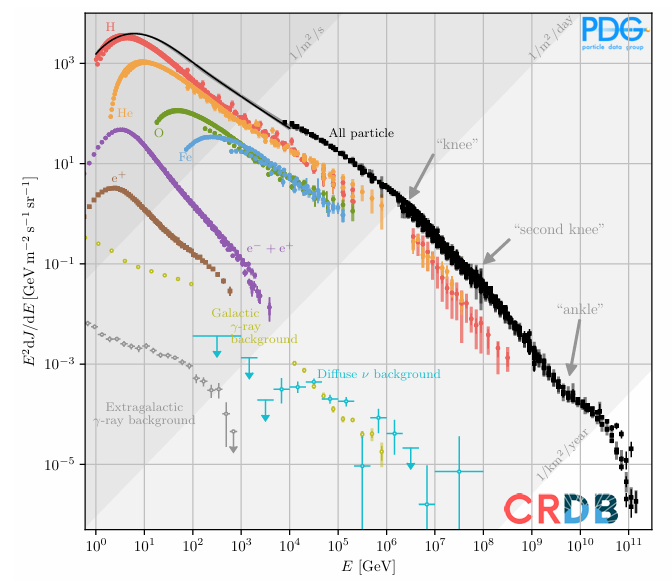
\includegraphics[width=0.65\linewidth]{figures/CRs-energy-spectrum.png}
    \caption[The cosmic ray energy spectrum.]{The cosmic ray energy spectrum. The intensity of charged and neutral cosmic rays, multiplied by kinetic energy squared, is shown as a function of energy. Characteristic breaks such as the knee, second knee, and ankle are clearly visible.}
    \label{fig:crs-spectrum}
\end{figure}

\subsection{Gamma Rays as Cosmic Ray Tracers}

A central motivation for gamma-ray astronomy in the context of cosmic ray physics is that photons, being electrically neutral, are not deflected by interstellar magnetic fields and therefore travel in straight lines from their production sites. This makes them valuable probes of cosmic ray acceleration environments. When a high-energy proton interacts with ambient matter near its source, it produces pions, and neutral pions decay promptly into photon pairs
\begin{equation}
    \pi^0 \to \gamma + \gamma,
\end{equation}
generating gamma-ray emission that directly reflects the parent proton spectrum. Detecting this hadronic signature from a source constitutes direct evidence of cosmic ray acceleration at that site.

However, high-energy electrons can also produce gamma rays through inverse Compton scattering\footnote{Inverse Compton scattering is the process by which a relativistic electron transfers energy to a low-energy photon, up-scattering it to gamma-ray energies; it is the leptonic counterpart to the hadronic $\pi^0$ channel.} and bremsstrahlung\footnote{Bremsstrahlung (German for ``braking radiation'') is the radiation emitted when a charged particle, typically an electron, is deflected by the electric field of an atomic nucleus.}, generating leptonic emission that closely resembles the hadronic signature spectrally. Distinguishing between the two is a central observational challenge, and it is precisely this challenge that motivates the task of gamma-hadron discrimination at ground-based detectors.

\subsection{The Sub-TeV Window}

The energy range between 100 GeV and a few TeV marks the boundary between what is accessible to space-based instruments and what requires ground-based observation. The Fermi-LAT, a space-based pair-conversion gamma-ray telescope 
operating aboard a satellite above the Earth’s atmosphere, effectively detects gamma rays up to a few hundred GeV but is limited by its collection area at higher energies~\shortcite{ackermann2012fermi}. Above this threshold, ground-based detectors exploit the EAS that cosmic rays and gamma rays produce in the atmosphere, reaching the detector level as measurable patterns of secondary particles. CONDOR is designed to operate precisely in this sub-TeV window, and the reconstruction of shower properties in this regime is the central problem addressed in this thesis.

\section{Physics of Extensive Air Showers}

When a high-energy primary particle enters the Earth's atmosphere, it does not reach the ground directly. Instead, its interaction with atmospheric nuclei initiates a cascade of secondary particles that propagates downward at nearly the speed of light, growing in number until the energy per particle drops below the threshold for further multiplication. These cascades, known as extensive air showers, are the fundamental observable that ground-based gamma-ray and cosmic ray observatories exploit~\shortcite{rossi1941cosmic}.

Figure~\ref{fig:cascade_tree} summarizes the sequence of processes that follow the first interaction. The primary produces a large multiplicity of secondary hadrons, mostly pions; the charged ones sustain the hadronic cascade and eventually decay into muons, while the neutral ones decay into photon pairs and transfer their energy into electromagnetic sub-cascades. The three components that reach the ground --- hadronic, muonic and electromagnetic --- are what a surface array actually samples, and the following subsections describe the electromagnetic and hadronic branches in turn.

\begin{figure}[ht!]
    \centering
    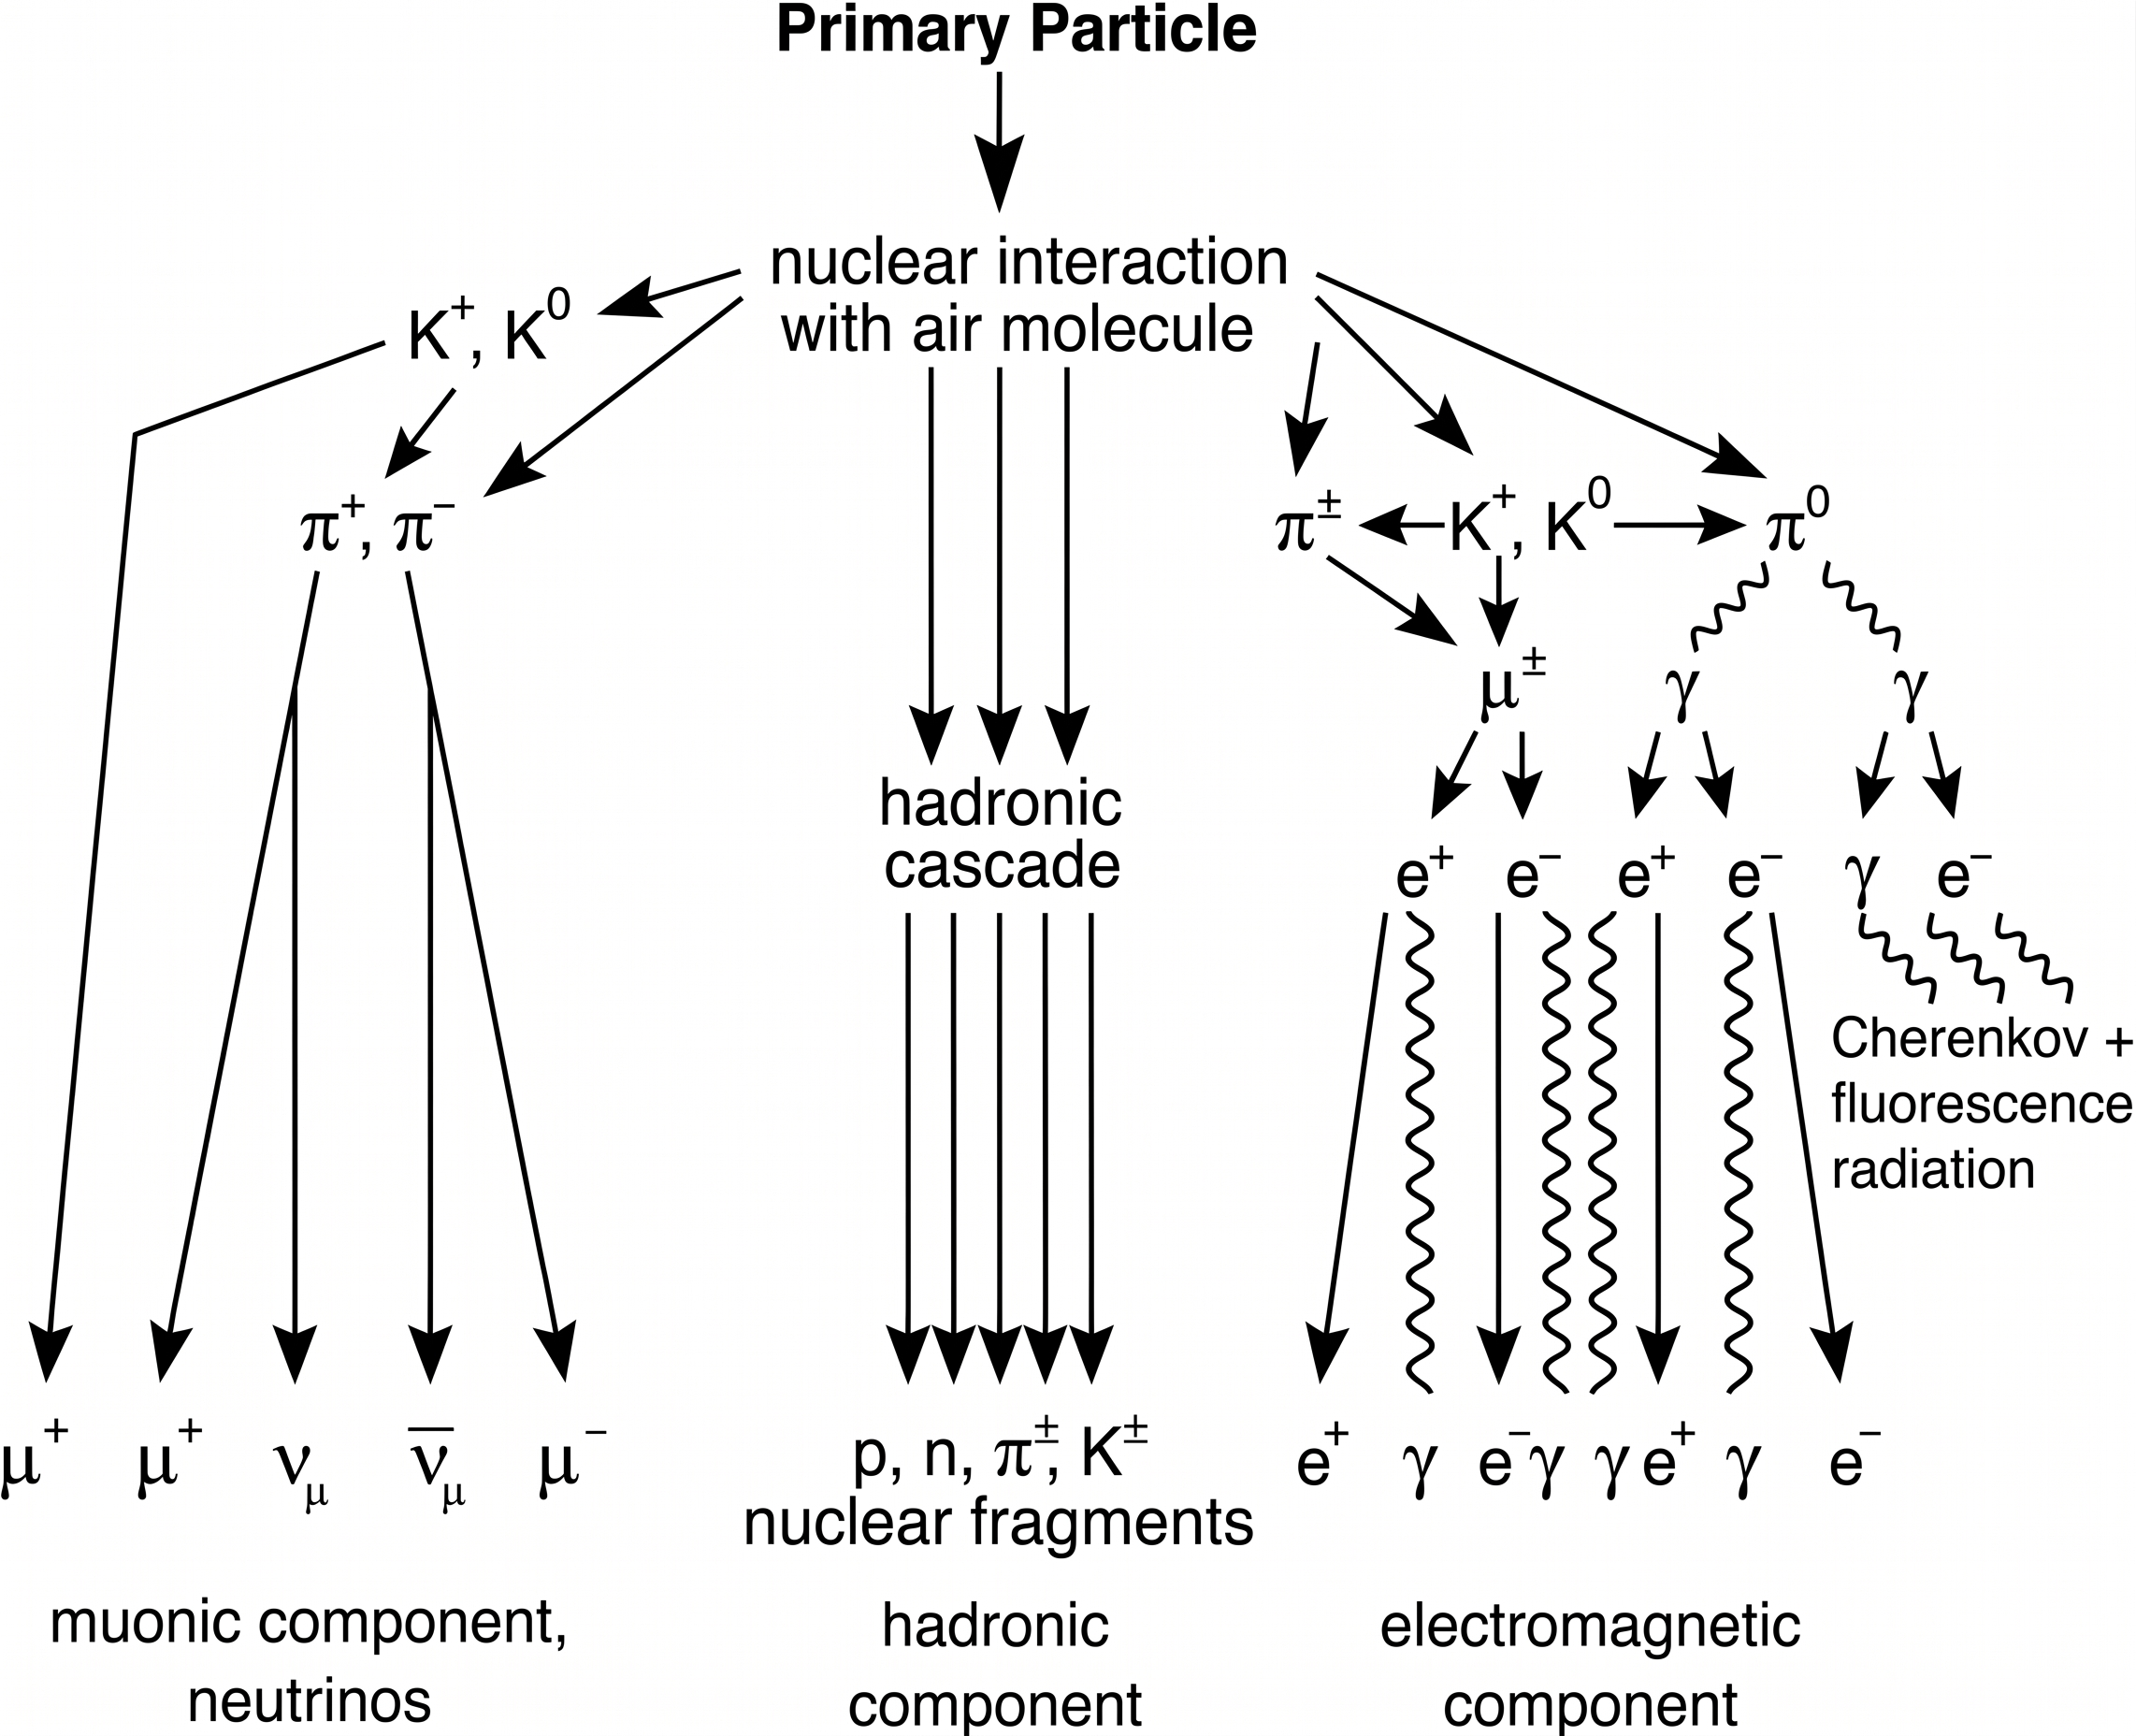
\includegraphics[width=0.85\linewidth]{figures/eas-diagram.png}
    \caption[Branching structure of an air shower.]{Branching structure of an air shower, grouped into the three components sampled at ground level. \textbf{Left:} the muonic and neutrino component. Charged kaons and pions ($K^{\pm}$, $K^{0}$, $\pi^{\pm}$) decay into muons and muon neutrinos, which are weakly interacting and reach the ground largely undisturbed. \textbf{Centre:} the hadronic component. Successive nuclear interactions sustain the hadronic cascade, whose surviving nucleons and mesons ($p$, $n$, $\pi^{\pm}$, $K^{\pm}$) constitute the nuclear fragments that reach the ground. \textbf{Right:} the electromagnetic component. Neutral pions decay promptly into photon pairs, which alternate pair production and bremsstrahlung to build an electron-positron-photon cascade; this component is what a Cherenkov or fluorescence detector observes directly, and what dominates the particle count of the shower.}
    \label{fig:cascade_tree}
\end{figure}

\subsection{Electromagnetic Showers}
\label{subsec:electromagnetic_showers}

The simplest type of EAS is initiated by a high-energy photon or electron. When a photon of sufficient energy passes close to an atmospheric nucleus, it converts into an electron-positron pair in the screened Coulomb field of that nucleus. This process, known as pair production, requires a photon energy of at least twice the electron rest mass ($2 m_e c^2 \approx 1.022$ MeV) and relies on the nearby nucleus to absorb the recoil momentum so that energy and momentum are simultaneously conserved. Each member of the resulting pair is then deflected in the same nuclear fields and radiates a bremsstrahlung photon, which can in turn produce a further pair, and so on. The cascade multiplies rapidly, roughly doubling the particle number at each step, until the energy per particle is no longer sufficient to sustain further pair production.

A useful framework for understanding this process is the Heitler model~\shortcite{heitler1984quantum, matthews2005heitler}, which describes the shower as a binary splitting process. After each splitting length, every particle splits into two secondaries of half the original energy. Starting from a primary of energy $E_0$, the shower reaches its maximum particle number when the energy per particle equals the critical energy $E_c$, below which ionization losses dominate over radiative processes. The number of generations required is $n = \log_2(E_0/E_c)$, so the maximum occurs at an atmospheric depth
\begin{equation}
    X_{\text{max}} = \frac{X_0}{\ln 2}\,\ln{\frac{E_0}{E_c}} \ ,
    \label{eq:xmax}
\end{equation}
measured in $\mathrm{g \ cm}^{-2}$ of traversed atmosphere, where $X_0$ is the radiation length\footnote{The radiation length is the mean atmospheric depth over which a high-energy electron loses all but a fraction $1/e$ of its energy through bremsstrahlung; it is the natural length scale of electromagnetic shower development.} and the factor $X_0/\ln 2$ is the effective splitting length of the cascade. The quantity $X_{\text{max}}$ is one of the most important observables in EAS physics: it depends logarithmically on the primary energy and is sensitive to the primary particle type, making it a key discriminant between electromagnetic and hadronic showers.

Shower development is tracked in units of \textit{atmospheric depth} rather than geometric distance, which is why $X_{\text{max}}$ carries units of $\mathrm{g \ cm}^{-2}$. Atmospheric depth is the mass of air per unit area contained in the column above a given point, and it is the natural coordinate for a cascade because the number of interactions a particle undergoes depends on how much matter it has crossed and not on how far it has moved. Appendix~\ref{sec:apx_depth} develops this in full, together with its two consequences for this work: the dependence of the traversed depth on the zenith angle, and the advantage of a high-altitude observation site.

\subsection{Hadronic Showers}
\label{subsec:hadronic_showers}

Showers initiated by protons or heavier nuclei are considerably more complex. The primary particle interacts inelastically with an atmospheric nucleus, producing a large multiplicity of secondary hadrons, predominantly pions. Charged pions $\pi^\pm$ continue the hadronic cascade through further inelastic interactions, while neutral pions $\pi^0$ decay almost immediately into photon pairs, seeding electromagnetic sub-showers at every generation. A hadronic shower is therefore a composite structure: a hadronic core that continuously feeds energy into a superposition of electromagnetic cascades developing at different depths.

This composite structure has two important consequences for detection. First, hadronic showers are intrinsically wider and more irregular in their lateral extent than purely electromagnetic showers, because hadronic interactions transfer significant transverse momentum and the multiple electromagnetic sub-showers develop independently along different axes. Second, a fraction of the primary energy is carried away by neutrinos produced in charged pion and muon decay, making hadronic showers less efficient at producing detectable particles at ground level than gamma-induced showers of the same primary energy. These morphological and energetic differences form the physical basis for gamma-hadron discrimination~\shortcite{rao1998extensive}.

Figure~\ref{fig:proton_vs_photon} illustrates these differences at the level of the ground detector array. The average footprint of gamma-induced showers is more compact and concentrated near the shower core, while proton-induced showers exhibit a broader, less symmetric lateral distribution and higher particle counts at peripheral detectors. The difference map (right panel) highlights the core-dominated excess for gamma events and the extended halo for hadronic events, providing a direct visual foundation for the morphological discrimination task.

\begin{figure*}[ht!]
    \centering
    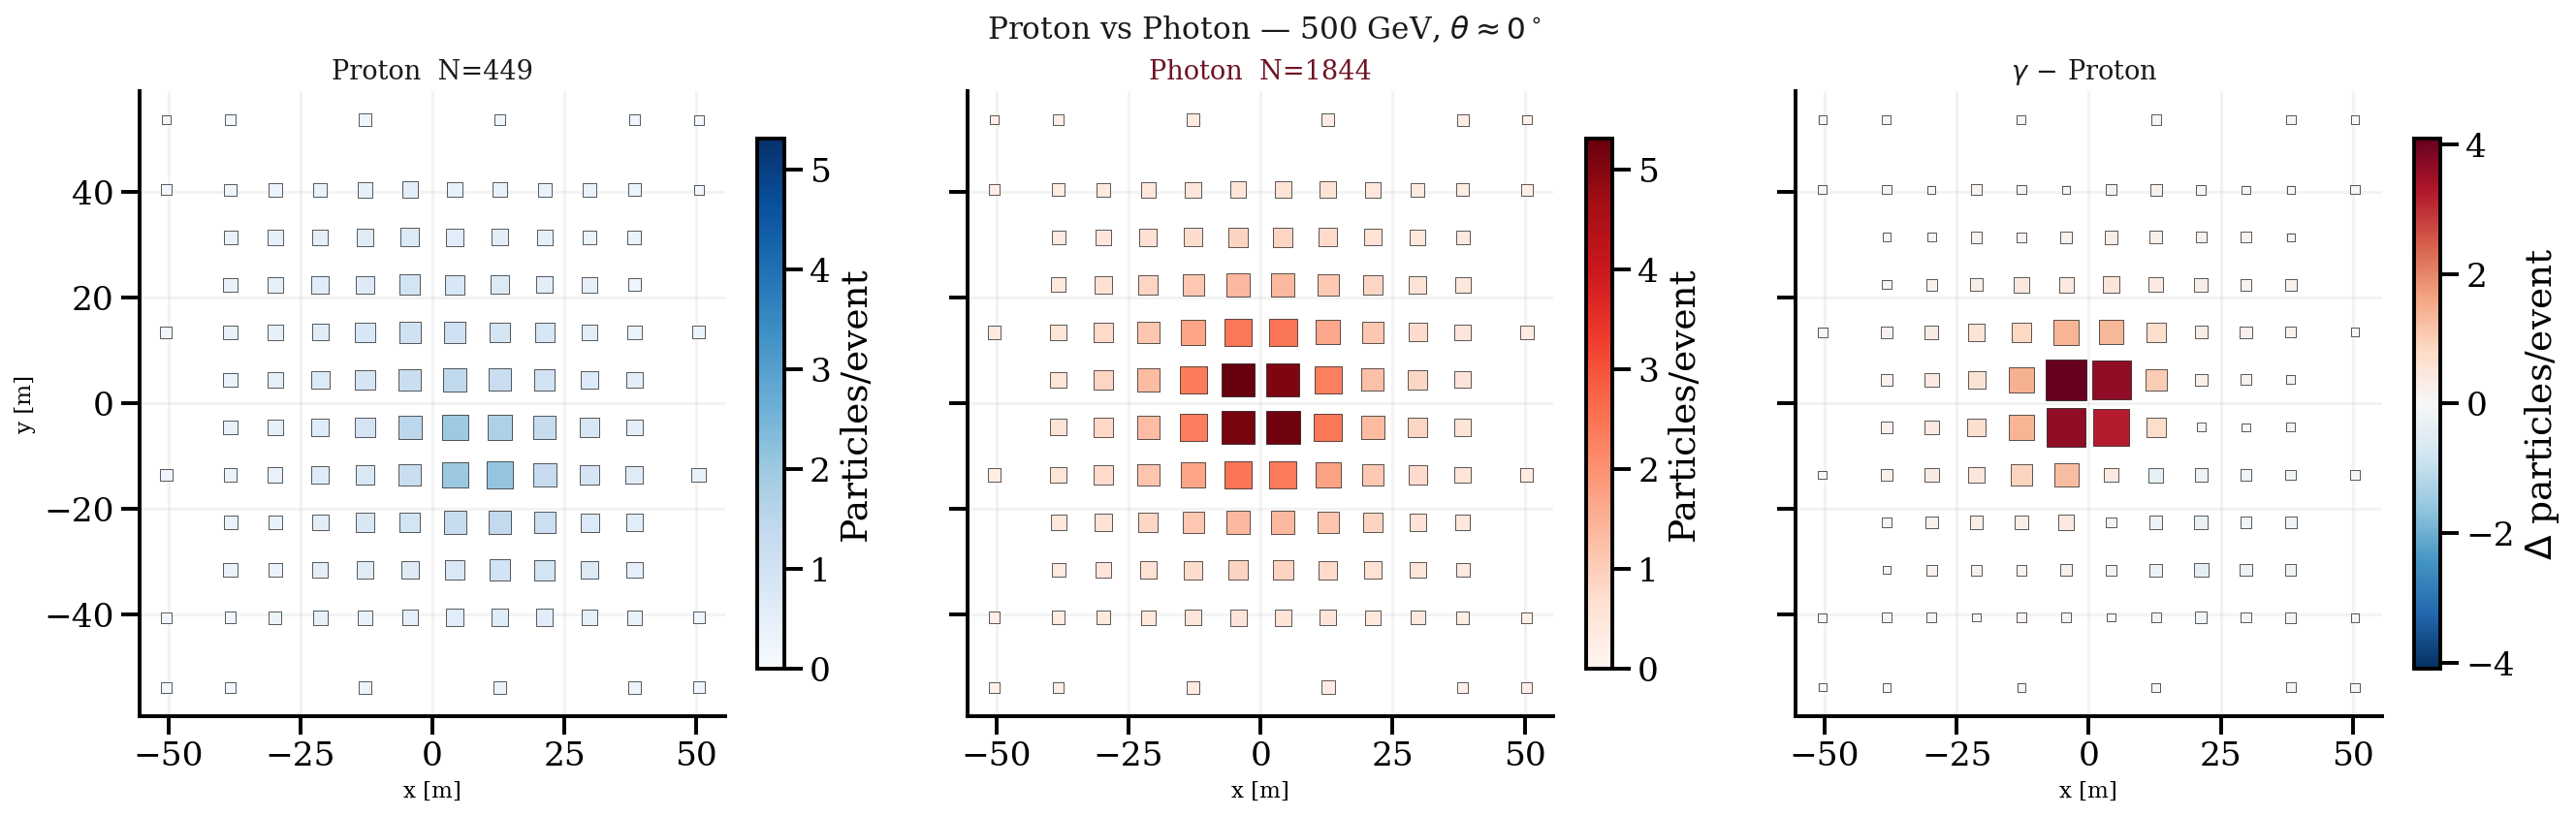
\includegraphics[width=1\linewidth]{figures/eas_proton_vs_photon.png}
    \caption[Average shower footprint: proton vs photon comparison.]{Average shower footprint at 500 GeV and $\theta \approx 0\degree$. \textbf{Left:} mean particle count per detector for proton-induced showers. \textbf{Center:} mean particle count per detector for gamma-induced showers. \textbf{Right:} difference map ($\gamma$ $-$ proton), revealing the more compact core signature of electromagnetic showers versus the wider lateral spread of hadronic showers. Marker size is proportional to particle count; position corresponds to physical detector location on the array.}
    \label{fig:proton_vs_photon}
\end{figure*}

\subsection{Shower Observables}

At ground level, an EAS manifests as a propagating disk of particles sweeping across the detector array and leaving a spatiotemporal pattern of hits. The key observables recorded by a surface array are the number of particles at each detector, the deposited energy, and the arrival time of the shower front.

The lateral distribution describes how the density of secondary particles varies with the distance from the shower core at the detector altitude. For the electromagnetic component of a shower, this distribution is well approximated by the Nishimura-Kamata-Greisen (NKG) function~\shortcite{nishimura1958kamata},
\begin{equation}
    \rho (r) = \frac{N_e}{2\pi r^2_{M}}\frac{\Gamma(4.5 - s)}{\Gamma(s) \Gamma(4.5-2s)}\qty(\frac{r}{r_M})^{s-2}\qty(1+\frac{r}{r_M})^{s-4.5},
    \label{eq:nkg}
\end{equation}
where $N_e$ is the total number of electrons, $r$ is the distance from the shower core, $r_M$ is the Molière radius,\footnote{The Molière radius is the characteristic transverse scale of an electromagnetic shower, defined as the radius of the cylinder around the shower axis that contains, on average, about 90\% of the deposited energy; it sets the lateral width of the particle distribution.} and $s$ is the shower age parameter that tracks the developmental stage of the cascade ($s = 1$ at shower maximum). The NKG function is relevant here as the classical parametric description of the lateral distribution: traditional reconstruction pipelines fit it to the measured hit pattern to estimate the shower size and core position. The deep learning model developed in this thesis does not fit any fixed functional form; instead, it learns the lateral and temporal structure of the shower directly from the detector hits, and therefore does not assume the shape given by the NKG function in advance. Figure~\ref{fig:lateral_distribution} shows the distribution predicted by this function.

\begin{figure*}[ht!]
    \centering
    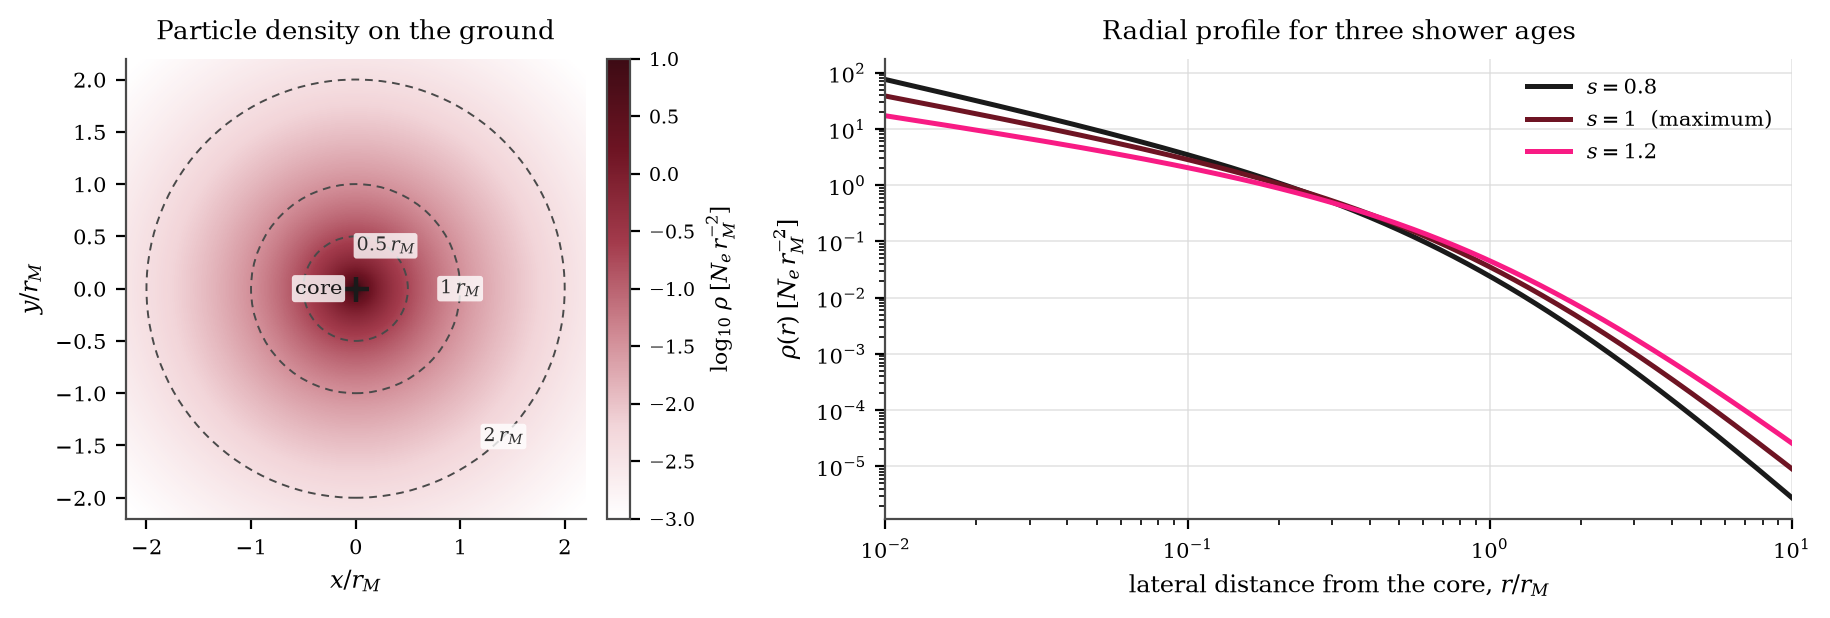
\includegraphics[width=1\linewidth]{figures/lateral_distribution.png}
    \caption[Lateral particle density predicted by the NKG function.]{Lateral particle density predicted by the NKG function of Equation~\ref{eq:nkg}, in units of the Moli\`ere radius $r_M$ so that it does not depend on the air density at the observation altitude. \textbf{Left:} density on the ground at shower maximum ($s = 1$), with rings at $0.5$, $1$ and $2\,r_M$. \textbf{Right:} radial profile for three shower ages: a young shower is more concentrated on the core, an older one flatter and wider.}
    \label{fig:lateral_distribution}
\end{figure*}

The timing of the shower front encodes the arrival geometry of the primary particle. As shown in Figure~\ref{fig:shower_geometry}, for an ideal planar front traveling at the speed of light, the arrival time difference between two detectors separated by a displacement vector $\Delta \textbf{r}$ is
\begin{equation}
    \Delta t = -\frac{\hat{n}\cdot \Delta \textbf{r}}{c},
    \label{eq:front}
\end{equation}
where $\hat{n}$ is the unit vector in the shower propagation direction. In practice, shower front curvature and stochastic fluctuations introduce deviations from this ideal model, but the timing information remains the primary observable for reconstructing the arrival direction of the incoming primary. In this thesis the azimuthal angle is held fixed in the simulations (Section~\ref{sec:corsika}), so the arrival-time gradient is exploited specifically for the reconstruction of the zenith angle $\theta$ --- one of the three target tasks of the model --- which is why this observable is emphasized here.

\begin{figure*}[ht!]
\centering
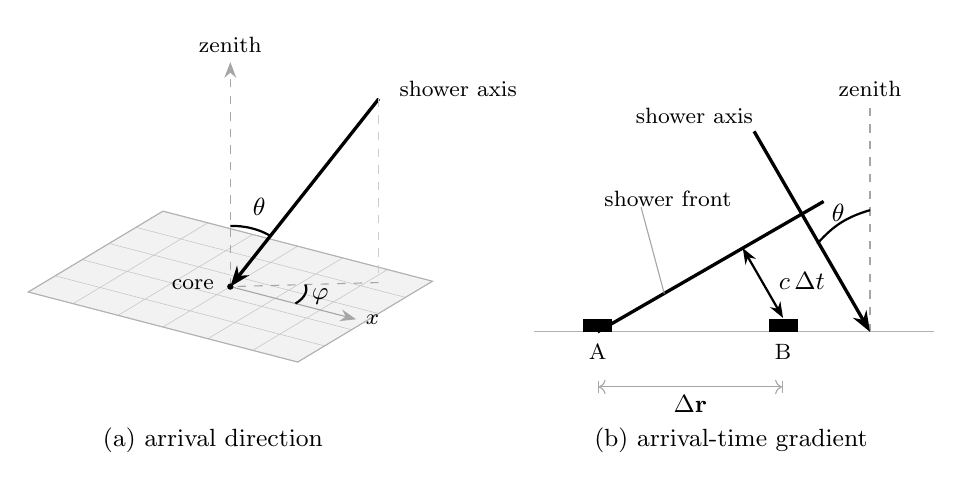
\begin{tikzpicture}[scale=0.92]

% ---- panel (a): three-dimensional view of the arrival direction ----
\begin{scope}[
    x={(1cm,-0.26cm)}, y={(0.60cm,0.36cm)}, z={(0cm,1cm)},
    scale=0.62]

  \fill[gray!10] (0,0,0) -- (6,0,0) -- (6,5,0) -- (0,5,0) -- cycle;
  \draw[gray!45, very thin]
    \foreach \i in {0,1,2,3,4,5,6} { (\i,0,0) -- (\i,5,0) }
    \foreach \j in {0,1,2,3,4,5} { (0,\j,0) -- (6,\j,0) };
  \draw[gray!60] (0,0,0) -- (6,0,0) -- (6,5,0) -- (0,5,0) -- cycle;

  \draw[dashed, gray!70, -{Stealth[length=2mm]}] (3,2.5,0) -- (3,2.5,5.0)
      node[above, font=\footnotesize, black] {zenith};

  \draw[very thick, -{Stealth[length=2.6mm]}]
      (5.20,4.34,4.09) -- (3,2.5,0);
  \node[font=\footnotesize, anchor=west] at (5.35,4.5,4.3) {shower axis};

  \draw[dashed, gray!70] (5.20,4.34,0) -- (3,2.5,0);
  \draw[dashed, gray!40] (5.20,4.34,4.09) -- (5.20,4.34,0);

  \draw[gray!70, -{Stealth[length=2mm]}] (3,2.5,0) -- (5.8,2.5,0)
      node[right, font=\footnotesize, black] {$x$};

  \draw[thick] plot coordinates {(3.000,2.500,1.350) (3.049,2.541,1.349) (3.097,2.581,1.344) (3.146,2.622,1.337) (3.194,2.662,1.326) (3.241,2.702,1.313) (3.288,2.741,1.297) (3.335,2.780,1.277) (3.381,2.818,1.256) (3.425,2.856,1.231) (3.469,2.893,1.203) (3.512,2.928,1.173) (3.554,2.963,1.141) (3.595,2.997,1.105)};
  \node[font=\small] at (3.427,2.857,1.764) {$\theta$};

  \draw[thick] plot coordinates {(4.450,2.500,0.000) (4.448,2.578,0.000) (4.442,2.655,0.000) (4.431,2.732,0.000) (4.417,2.808,0.000) (4.398,2.884,0.000) (4.376,2.958,0.000) (4.349,3.031,0.000) (4.319,3.103,0.000) (4.285,3.172,0.000) (4.247,3.240,0.000) (4.205,3.306,0.000) (4.160,3.369,0.000) (4.112,3.430,0.000)};
  \node[font=\small] at (4.645,3.097,0) {$\varphi$};

  \fill (3,2.5,0) circle (2.0pt);
  \node[font=\footnotesize, anchor=east] at (2.85,2.5,0) {core};
\end{scope}
\node[font=\small] at (2.55,-2.05) {(a) arrival direction};

% ---- panel (b): side view of the shower front ----
\begin{scope}[xshift=6.9cm, yshift=-0.55cm, scale=0.80]

  \draw[gray!60] (0.1,0) -- (7.0,0);
  \fill[black] (0.95,0) rectangle ++(0.5,0.22);
  \node[font=\footnotesize, below] at (1.20,-0.04) {A};
  \fill[black] (4.15,0) rectangle ++(0.5,0.22);
  \node[font=\footnotesize, below] at (4.40,-0.04) {B};

  \draw[dashed, gray!70] (5.9,0) -- (5.9,3.9)
      node[above, font=\footnotesize, black] {zenith};

  \draw[very thick, -{Stealth[length=2.6mm]}] (3.9,3.46) -- (5.9,0);
  \node[font=\footnotesize, anchor=south east] at (4.05,3.42) {shower axis};

  \draw[thick] (5.9,2.1) to[bend right=16] (4.99,1.52);
  \node[font=\small] at (5.35,2.05) {$\theta$};

  \draw[very thick] (1.20,0) -- (5.10,2.25);
  \node[font=\footnotesize, anchor=west] at (1.15,2.30) {shower front};
  \draw[gray!70, thin] (1.95,2.15) -- (2.35,0.66);

  \draw[{Stealth[length=2mm]}-{Stealth[length=2mm]}, thick] (4.40,0.24) -- (3.704,1.446);
  \node[font=\small, anchor=west] at (4.16,0.88) {$c\,\Delta t$};

  \draw[|<->|, gray!70] (1.20,-0.95) -- (4.40,-0.95);
  \node[font=\small, below] at (2.80,-0.93) {$\Delta \mathbf{r}$};
\end{scope}
\node[font=\small] at (9.7,-2.05) {(b) arrival-time gradient};

\end{tikzpicture}
\caption[Arrival geometry of an extensive air shower.]{Arrival geometry of an extensive air shower. \textbf{(a)} The direction of the primary is given by the zenith angle $\theta$, from the vertical, and the azimuth $\varphi$, on the plane of the array; the axis meets that plane at the core. \textbf{(b)} Side view. The front is perpendicular to the axis, so it reaches A first and still has $c\,\Delta t$ to travel before reaching B; that delay is the projection of their separation onto the direction of propagation, Equation~\ref{eq:front}. Here $\varphi$ is fixed at $0\degree$ (Section~\ref{sec:corsika}), so only $\theta$ is reconstructed.}
\label{fig:shower_geometry}
\end{figure*}

Figure~\ref{fig:angle_evolution} shows how the average shower footprint evolves with the zenith angle for 500 GeV proton-induced showers simulated at CONDOR. As $\theta$ increases, the footprint elongates along the projection of the shower axis onto the detector plane, the lateral spread widens, and the arrival-time gradient across the array steepens. These systematic morphological changes underlie the angular reconstruction task addressed in this thesis.

\begin{figure*}[ht!]
    \centering
    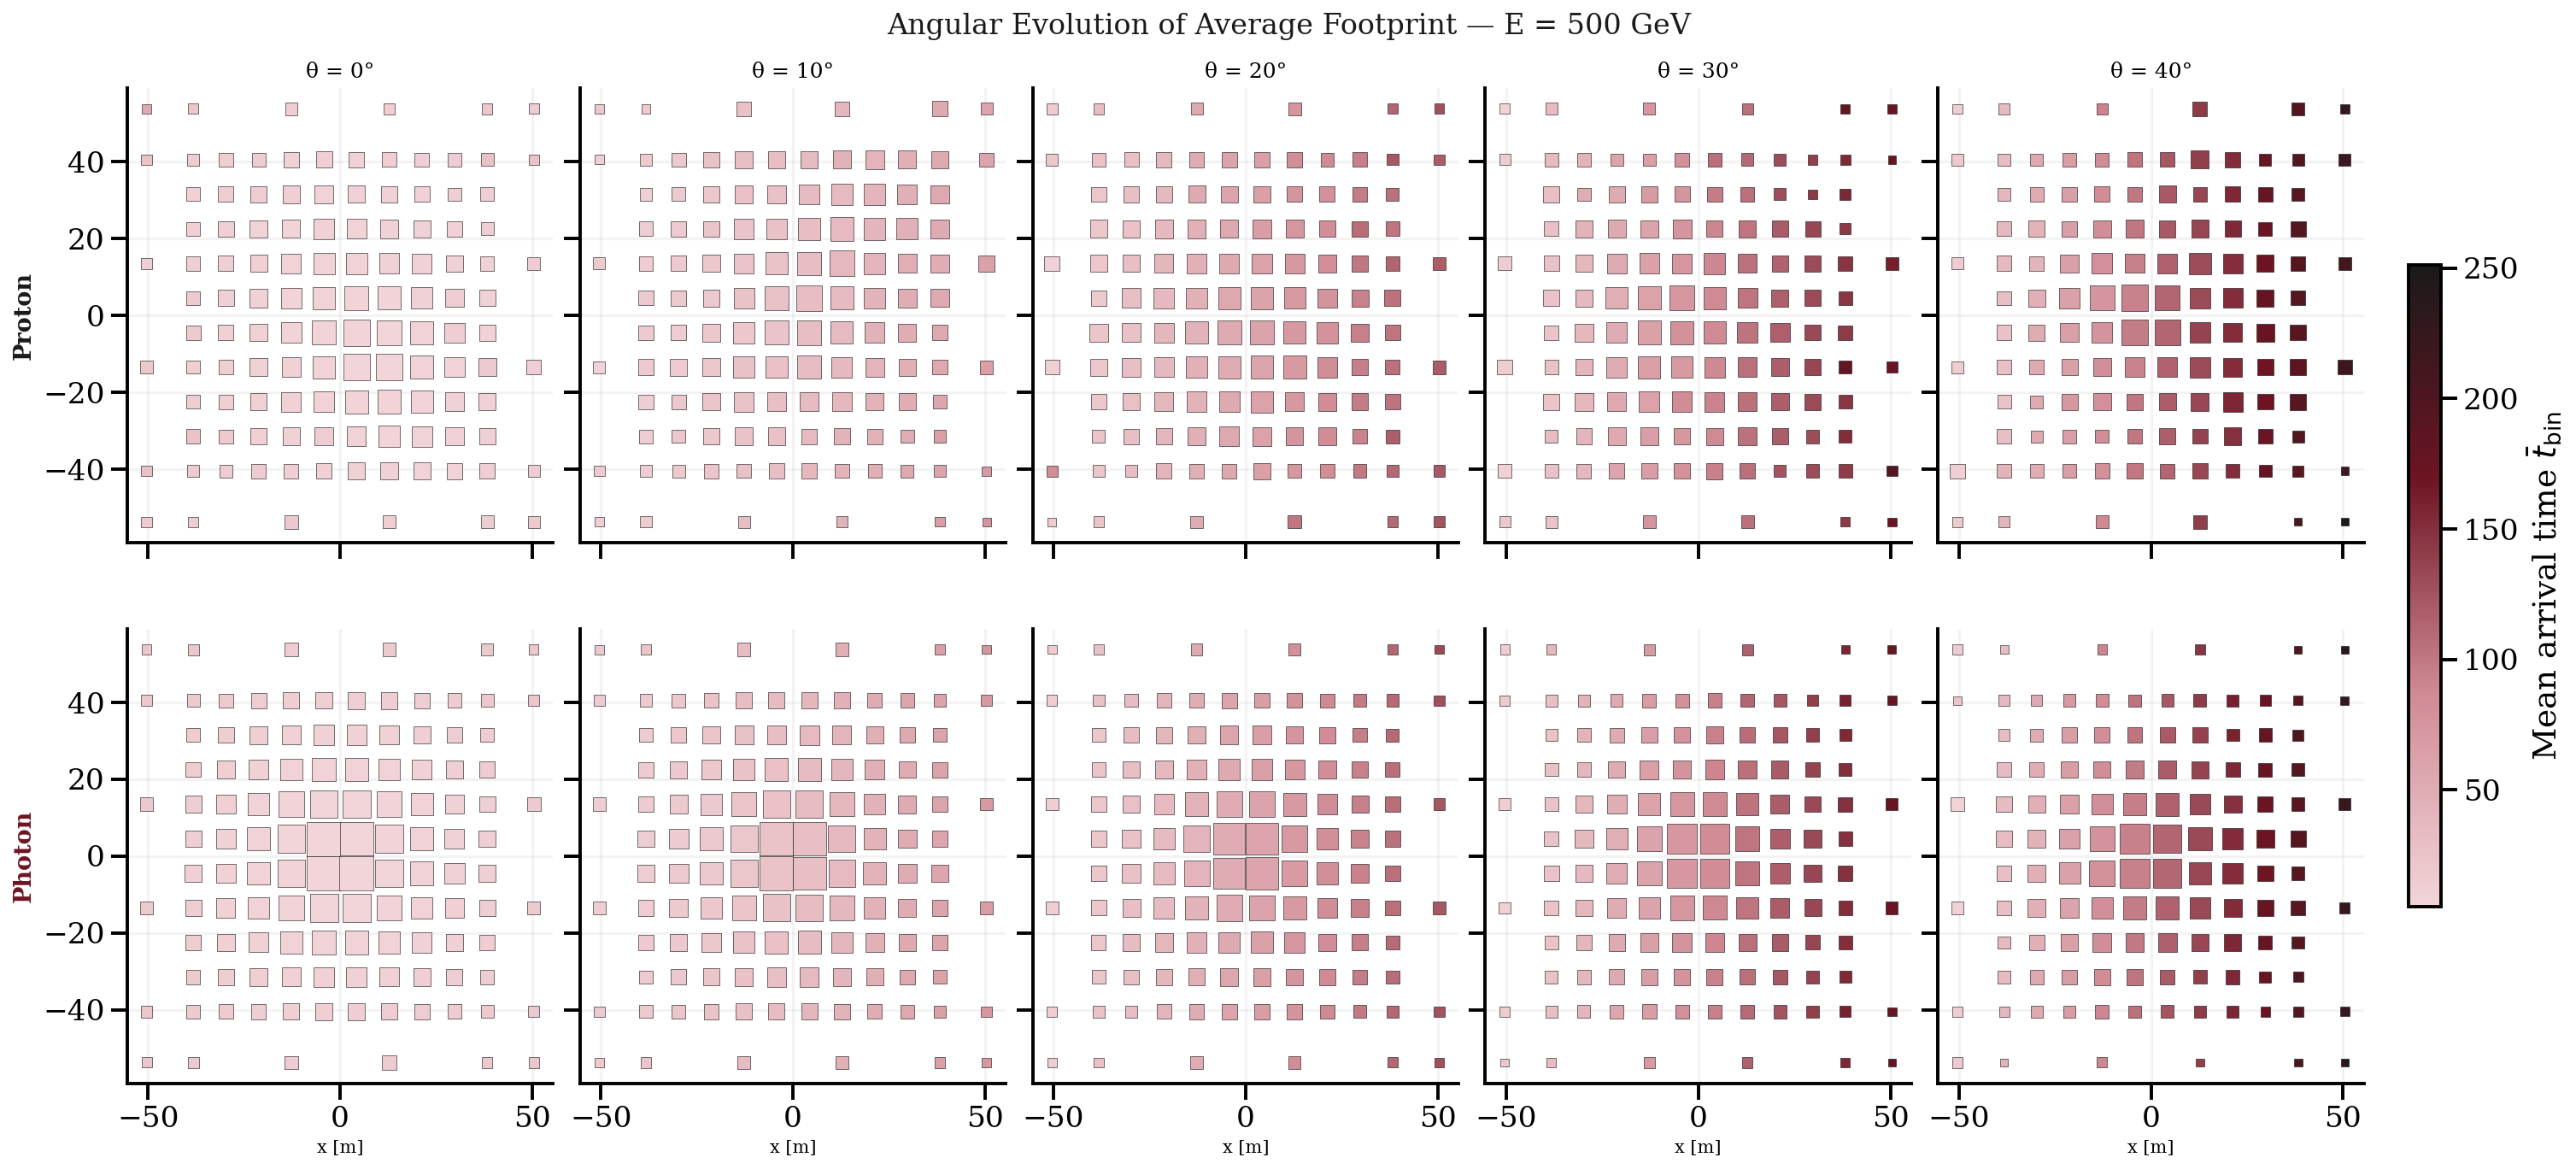
\includegraphics[width=1\linewidth]{figures/eas_angle_evolution.png}
    \caption[Angular evolution of the average EAS footprint.]{Angular evolution of the average shower footprint for proton-induced events at $E = 500\,\text{GeV}$. Each panel shows the mean particle count per detector averaged over all events within the corresponding zenith angle bin ($\theta \approx 0\degree$, $10\degree$, $20\degree$, $30\degree$, $40\degree$). As the zenith angle increases, the shower footprint elongates along the projected shower axis and the lateral spread broadens, providing the morphological signature exploited for zenith angle reconstruction. Color encodes the mean arrival time $\bar{t}_\mathrm{bin}$; marker size is proportional to particle count.}
    \label{fig:angle_evolution}
\end{figure*}

\section{Ground-Based Detection of EAS}

Ground-based observatories exploit the EAS as an indirect measurement device: rather than detecting the primary particle directly, they sample the shower footprint at ground level and use the recorded hit pattern to infer the properties of the primary cosmic ray, such as its type, energy, and arrival direction. This approach enables observation over large sky areas simultaneously and is not limited by collection area in the way that satellite detectors are.

In the sub-TeV and TeV energy regimes, ground-based arrays fall into two dominant technology categories. Water Cherenkov detectors, used by observatories such as HAWC~\shortcite{HAWK} and LHAASO~\shortcite{cao2022largehighaltitudeair}, consist of large tanks of purified water in which secondary particles produce Cherenkov light\footnote{Cherenkov light is the faint electromagnetic radiation emitted when a charged particle traverses a medium faster than the local phase velocity of light in that medium; its intensity and angular profile encode the particle's velocity and direction.} recorded by photomultiplier tubes. They offer good muon sensitivity, which is advantageous for gamma-hadron discrimination, but require large structural investment at high altitude. The same technology has been adopted for the Southern Wide-field Gamma-ray Observatory (SWGO)~\shortcite{SWGO}, a next-generation array proposed for the southern hemisphere, which would extend this coverage to a sky region that HAWC and LHAASO cannot observe. Plastic scintillator arrays, used by operating observatories such as Tibet AS$\gamma$~\shortcite{amenomori2019first} and adopted for the future CONDOR array~\shortcite{arratia2025condor}, consist of segmented scintillator panels that produce light pulses when charged particles pass through them, read out by silicon photomultipliers (SiPMs) through wavelength-shifting fibers. Scintillator arrays offer better timing resolution, higher modularity, and lower deployment weight than water Cherenkov detectors, making them suitable for operation at the highest altitudes.

\section{The CONDOR Observatory}
\label{sec:condor_observatory}

The CONDOR (\textbf{CO}mpact \textbf{N}etwork of \textbf{D}etectors with \textbf{O}rbital \textbf{R}ange) observatory is a proposed high-altitude gamma-ray and cosmic ray array designed to observe EAS in the 100 GeV to 1 TeV range~\shortcite{arratia2025condor}. It is currently in its design and validation phase, so all data used in this thesis are generated through Monte Carlo simulations that reproduce the expected response of the CONDOR array under its planned high-altitude operating conditions; the simulation framework is described in detail in Section~\ref{sec:corsika}. Figure~\ref{fig:condor-array} shows a schematic representation of the array layout.

\begin{figure}[ht!]
    \centering
    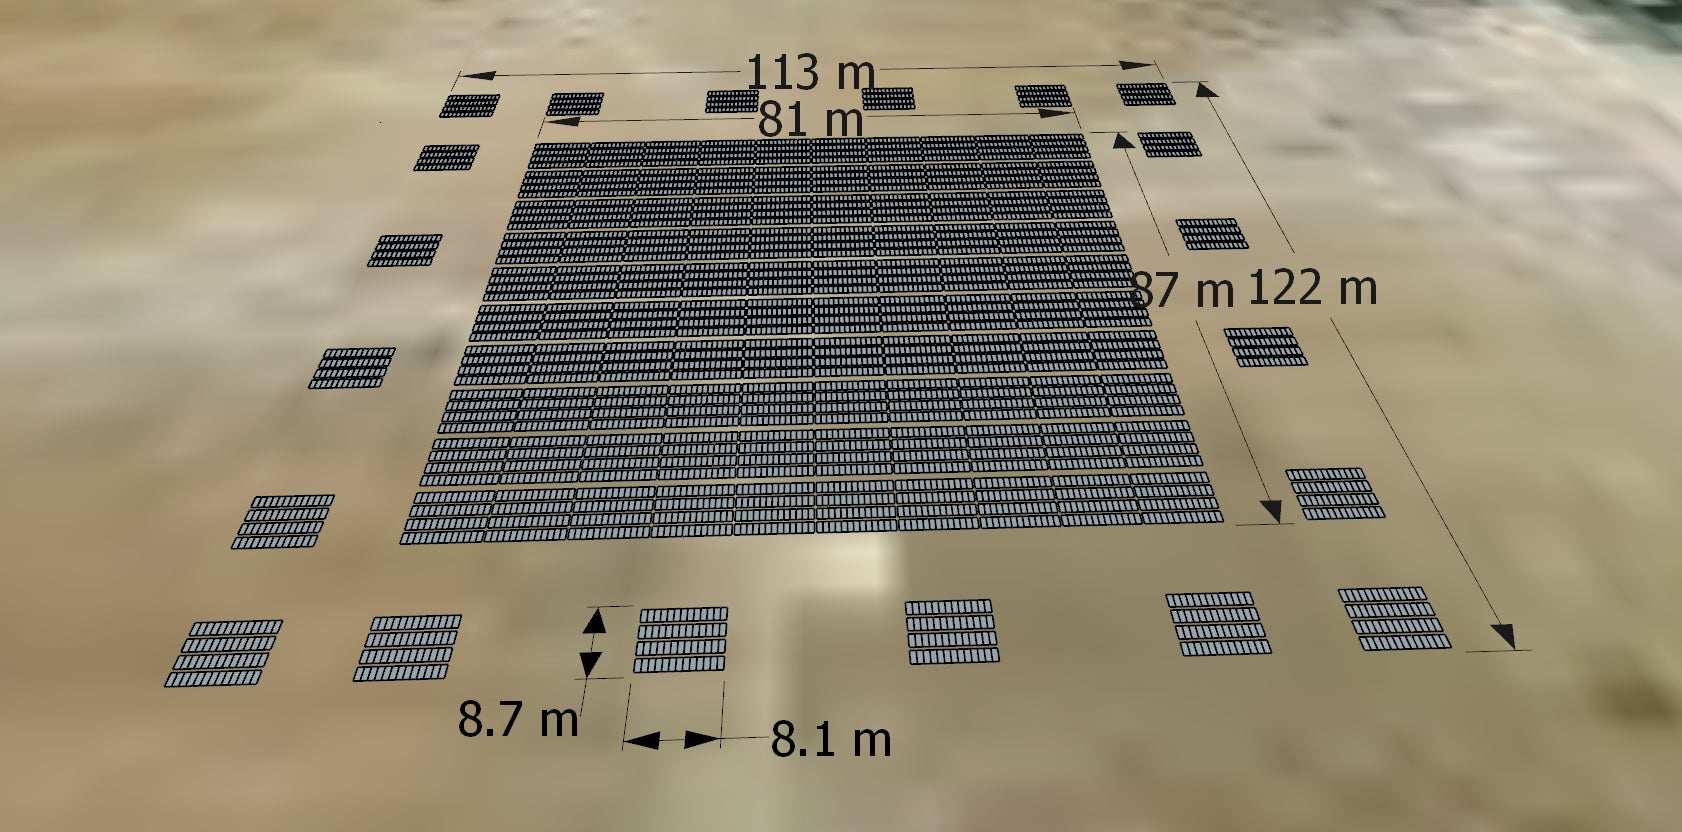
\includegraphics[width=0.95\linewidth]{figures/condor_img_2.png}
    \caption[Schematic of the CONDOR detector array layout.]{Schematic representation of the CONDOR observatory layout. The array achieves a high fill factor in its inner region using thousands of plastic scintillator units, surrounded by an outer veto ring to suppress backgrounds. Source: CONDOR Observatory~\shortcite{arratia2025condor}.}
    \label{fig:condor-array}
\end{figure}

\subsection{Design and High-Altitude Advantage}

CONDOR will be located within the Atacama Astronomical Park at Cerro Toco, Chile, at an altitude of 5,300 meters above sea level, placing it above established facilities such as HAWC at 4,100 m and LHAASO at 4,410 m. This altitude is the central design advantage of CONDOR. The number of secondary electrons reaching the ground level depends strongly on atmospheric depth: by operating closer to the shower maximum $X_{\text{max}}$, CONDOR avoids the progressive attenuation experienced by cascades traveling to lower elevations. This enables CONDOR to lower its effective energy threshold to approximately 100 GeV, accessing a range that is difficult to reach for lower-altitude arrays and that partially overlaps with the upper sensitivity limit of space-based gamma-ray instruments such as the Fermi-LAT.

\subsection{Array Layout and Detector Architecture}

The CONDOR array consists of 5,300 plastic scintillator detector units arranged in a compact central grid covering an area of approximately 6,000 $\mathrm{m}^2$, supplemented by 1,040 additional peripheral units forming a veto ring that encloses a total instrumented area of 14,000 $\mathrm{m}^2$. The central region achieves a fill factor of 90\%, meaning that nearly the entire surface is actively sensitive to shower particles. This high fill factor is essential for low-energy operation, where the shower footprint is small and sparse hits must be captured efficiently.

For the purpose of simulation and reconstruction, these individual detector units are grouped into \textbf{detector modules}, each covering an area of approximately $8.1 \times 8.7~\mathrm{m}^2$. As shown in Figure~\ref{fig:condor-modules}, the full array comprises 120 modules: 100 arranged in a $10 \times 10$ central grid, plus 20 peripheral modules. Each module aggregates the signals from its constituent scintillator panels into a single readout channel.

\begin{figure}[ht!]
    \centering
    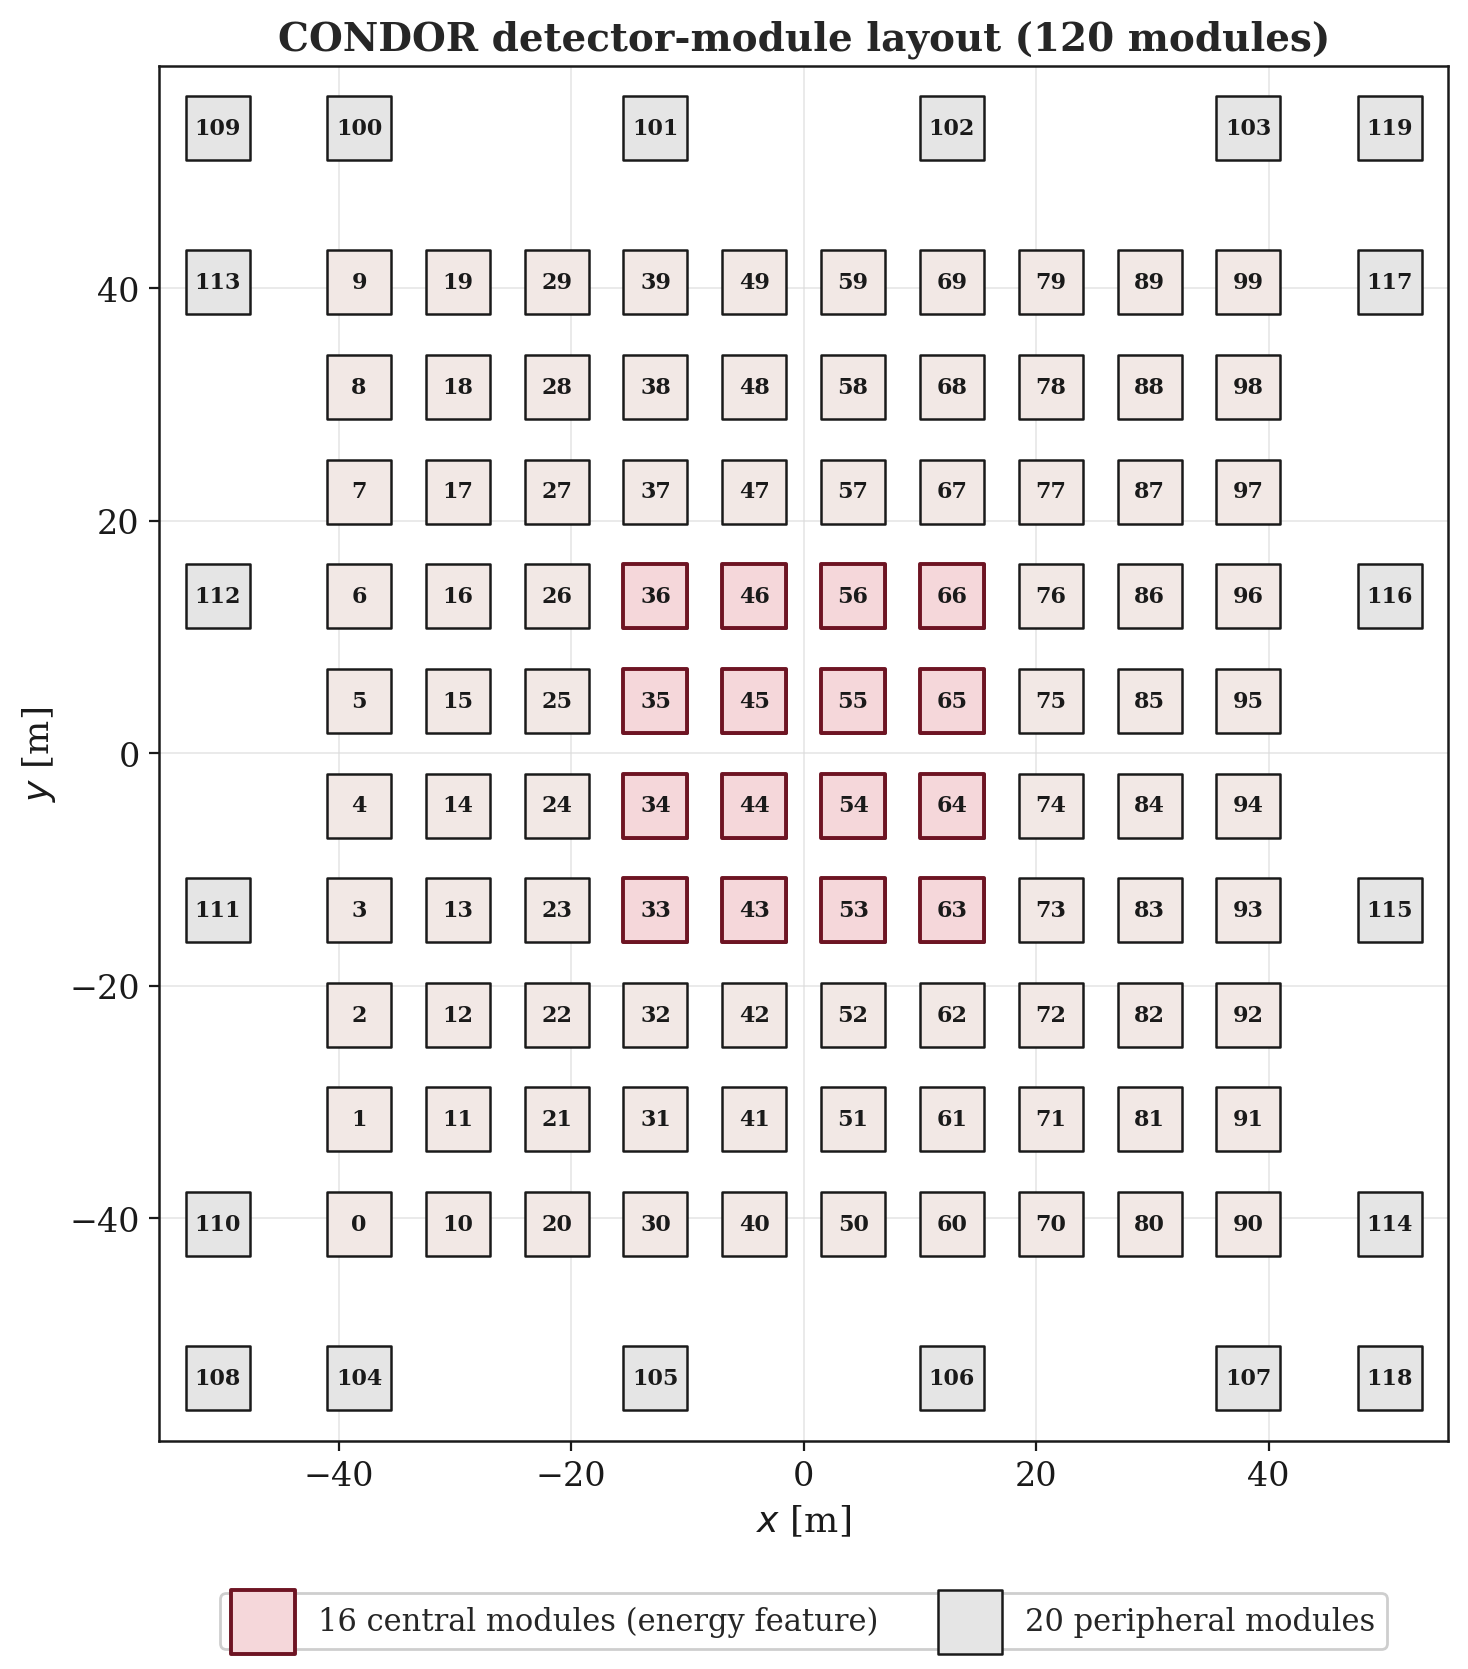
\includegraphics[width=0.85\linewidth]{figures/condor_modules_grid.png}
    \caption[Simulated CONDOR detector-module geometry and identifiers.]{Simulated CONDOR detector-module geometry used throughout this thesis. The 100 central modules (identifiers 0--99) form a $10 \times 10$ grid spanning approximately $87 \times 81~\mathrm{m}^2$, surrounded by 20 peripheral modules (identifiers 100--119), matching the planned observatory configuration. Each module aggregates the signals of its constituent scintillator units into a single readout channel. The module identifier is used directly as the \texttt{detector\_id} input feature of the model.}
    \label{fig:condor-modules}
\end{figure}

It is important to distinguish the two levels at which the shower is represented. The CORSIKA simulation itself does not know about detector modules: it tracks the air shower as individual particles and records their type, energy, and arrival position and time at the ground. The mapping onto the 120 detector modules is performed afterwards, during the data-processing stage, where the raw particle hits falling within each module's footprint are aggregated into the per-module quantities used by the model (Chapter~\ref{ch:methodology}). Throughout this thesis, the term \textit{detector} therefore refers to these modules unless otherwise specified, and the analysis operates at the module level rather than at the level of individual scintillator units or raw particle hits.

Each detector unit consists of extruded plastic scintillator bars, each coated with a 0.25 $\mathrm{mm}$ layer of titanium dioxide to enhance internal light reflection. A wavelength-shifting optical fiber runs through a central hole in each bar, collecting the fluorescent light produced by ionizing particles and guiding it to a silicon photomultiplier. The chosen SiPM model, the Hamamatsu S14160-6015PS, features 159,565 pixels and a photon detection efficiency of 32\%, providing single-photon sensitivity and precise timing. The units are enclosed in 5 $\mathrm{mm}$ aluminum housings for protection against the harsh Atacama environment, including the large daily temperature variations that require remote bias voltage adjustments to maintain stable detector performance.

\subsection{Data Acquisition and Sub-Nanosecond Synchronization}

Reconstructing the arrival direction of a shower front traveling at nearly the speed of light requires timing accuracy across thousands of detector nodes separated by tens to hundreds of meters. The intrinsic time resolution of each CONDOR unit is designed to be below one nanosecond, and sub-nanosecond synchronization across the full array is therefore a system-level requirement.

CONDOR is designed to achieve this through White Rabbit technology~\shortcite{moreira2009white}, an Ethernet-based timing protocol based on the IEEE 1588 standard\footnote{IEEE 1588, also known as the Precision Time Protocol (PTP), is an international standard for synchronizing clocks across nodes of a packet-switched network to sub-microsecond accuracy.} that distributes a pulse-per-second signal derived from the Global Positioning System (GPS) through fiber optic cables to White Rabbit nodes distributed across the array. Each node serves approximately ten detector panels, providing sub-nanosecond timing to each readout board. This synchronization allows offline discrimination between genuine shower hits and uncorrelated dark noise pulses, and it is the foundation on which the timing-based reconstruction of arrival direction depends.

\section{The CORSIKA Simulation Framework}
\label{sec:corsika}

Because the CONDOR observatory has not yet begun scientific operations, all data used in this thesis are generated through Monte Carlo simulation. The simulation tool is CORSIKA (COsmic Ray SImulations for KAscade), developed at the Karlsruhe Institute of Technology and the standard framework for EAS simulation across the ground-based cosmic ray and gamma-ray community~\shortcite{Heck1998}.

CORSIKA tracks the propagation, interaction, and decay of every secondary particle produced in the cascade, from the first interaction of the primary in the upper atmosphere down to a configurable observation level. The cascade is treated as a set of coupled components --- hadronic, electromagnetic, and muonic --- each governed by the relevant physics. Hadronic interactions are split into two energy regimes handled by different interaction models matched at a transition energy. The high-energy regime --- the first, most energetic collisions of the primary and its leading secondaries --- is simulated with the EPOS model~\shortcite{pierog2009epos}, which provides a comprehensive treatment of minijet production, string fragmentation, and nuclear effects. The low-energy regime --- the more numerous, softer interactions that dominate the later stages of shower development --- is handled by the GHEISHA model~\shortcite{fesefeldt1985gheisha}. The neutral pions produced in these hadronic interactions decay almost immediately into photon pairs and feed the electromagnetic component, whose pair-production and bremsstrahlung sub-cascades are followed explicitly down to user-defined energy thresholds, below which particles are no longer tracked. The atmosphere is modeled as a series of layers with exponentially varying density, and the observation level is set to 5,300 m above sea level to match the planned altitude of CONDOR.

Conceptually, CORSIKA provides a full Monte Carlo realization --- with all the stochastic fluctuations of real showers --- of the average cascade development captured analytically by the Heitler model introduced earlier in this chapter. Whereas the Heitler model yields the mean depth of shower maximum and the mean particle number as smooth functions of primary energy, CORSIKA samples individual showers event by event, reproducing the shower-to-shower variability and the correlations between observables that the reconstruction model must learn to exploit.

The simulations cover proton and gamma-ray primaries at three discrete energies, 300, 500, and 800 GeV, with zenith angles sampled at uniform intervals from $0\degree$ to $40\degree$ in steps of $2\degree$, producing 21 discrete inclinations, and the azimuthal angle fixed at $\phi = 0\degree$. Events producing fewer than 30 secondary particles at the observation level are discarded. The full dataset construction and balancing procedure is described in Chapter~\ref{ch:methodology}.

\section{Convolutional Neural Networks}

Convolutional neural networks (CNNs) are a class of deep learning architectures designed to process data with local spatial or temporal structure~\shortcite{lecun1998convolutional}. Their defining property is the use of shared learned filters applied across the input, which allows the network to detect the same local pattern regardless of where it appears in the sequence. In this thesis, a CNN backbone is used to extract local temporal features from the ordered sequence of detector hits that constitutes the primary input to the reconstruction model.

\textbf{The convolution operation.} For a one-dimensional input sequence $\textbf{x} \in \mathbb{R}^{T\times C_{\text{in}}}$, where $T$ is the sequence length and $C_{\text{in}}$ is the number of input channels, and a learned filter $\textbf{w} \in \mathbb{R}^{k\times C_{\text{in}}\times C_{\text{out}}}$ of kernel size $k$, the output at position $t$ for output channel $j$ is
\begin{equation}
    y_j(t) = \sum_{c=1}^{C_\text{in}} \sum_{i=0}^{k-1} w_{i,c,j} \cdot x_{t+i,c} + b_j,
\end{equation}
where $b_j$ is learnable bias. The filter $\textbf{w}$ is shared across all positions $t$, which gives CNNs two important properties: translational equivariance, meaning that a pattern detected at one position will also be detected if it appears elsewhere in the sequence, and a substantially reduced parameter count compared to a fully connected network operating on the same input.

\textbf{Pooling and normalization.} Following each convolution, max pooling reduces the temporal resolution by selecting the maximum activation within non-overlapping windows of size $p$,
\begin{equation}
    z_j(t) = \max_{0\leq i <p}{ y_j (tp +i)} \ ,
\end{equation}
retaining the presence and magnitude of detected features while discarding fine positional detail. Batch normalization~\shortcite{ioffe2015batch} then standardizes each feature map across the batch dimension before applying learnable scale and shift parameters,
\begin{equation}
    \hat{y}_j = \frac{y_j - \mu_j}{\sqrt{\sigma^2_j + \epsilon}}, \quad \tilde{y}_j = \gamma_j \hat{y}_j + \beta_j
\end{equation}
where $\mu_j$ and $\sigma^2_j$ are the batch mean and variance for channel $j$, and $\gamma_j, \beta_j$ are trainable. Batch normalization stabilizes training and permits higher learning rates without destabilizing the optimization. It was originally motivated as a way to reduce internal covariate shift, although subsequent work attributes its effect primarily to a smoothing of the optimization landscape rather than to covariate-shift reduction.

\textbf{Activation.} The nonlinearity applied after normalization is the Exponential Linear Unit (ELU)~\shortcite{clevert2015fast},

\begin{equation}
    \text{ELU}(x) = \begin{cases}
        x & \text{if} \ x >0 , \\
        \alpha(e^x - 1) & \text{if} \ x \leq 0,
    \end{cases}
\end{equation}
where the scale parameter $\alpha$ controls the saturation value for negative inputs; the standard choice $\alpha = 1$ is used, which makes the activation continuously differentiable at $x = 0$ (the left derivative $\alpha e^{x}|_{x=0} = \alpha$ matches the right derivative of $1$) and sets the negative saturation level to $-1$. Unlike the rectified linear unit (ReLU), ELU produces negative outputs for negative inputs, preserving a non-zero mean activation and accelerating convergence in deep networks by reducing the bias shift effect.

The specific CNN architecture used in this work, including the number of layers, filter configurations, and projection heads, is detailed in Chapter~\ref{ch:methodology}.

\section{Transformer Architectures}
\label{sec:transformer}

The Transformer is a deep learning architecture introduced by~\shortciteA{vaswani2017attention} that processes sequences through scaled dot-product attention. Unlike recurrent architectures such as long short-term memory networks~\shortcite{hochreiter1997long}, which propagate information sequentially through a hidden state and struggle with long-range dependencies, the Transformer computes all pairwise interactions between sequence positions in parallel, making it both more expressive for long-range structure and more efficient on modern hardware. In this thesis, Transformer streams process both the CNN-extracted feature sequence and the raw masked hit sequence to capture global temporal dependencies across the full shower hit pattern; the full multi-stream configuration is detailed in Chapter~\ref{ch:methodology}.

\textbf{Scaled dot-product attention.} The input to the attention mechanism is a sequence of \textit{token embeddings}: vector representations of the discrete elements of the sequence (in this work, each token corresponds to one detector hit, encoded either as its raw feature vector or as a CNN-derived feature embedding). Three learned linear projections map this sequence to queries, keys, and values: the \textit{query} of a position asks ``what information am I looking for?'', the \textit{key} of every other position answers ``what information do I expose?'', and the \textit{value} carries the actual content that will be propagated. Concretely, the three projections produce $\textbf{Q} \in \mathbb{R}^{T \times d_k}$, $\textbf{K} \in \mathbb{R}^{T \times d_k}$, and $\textbf{V} \in \mathbb{R}^{T \times d_v}$, and the attention output is
\begin{equation}
    \text{Attention}(\textbf{Q}, \textbf{K}, \textbf{V}) = \text{softmax}\qty(\frac{\textbf{QK}^\top}{\sqrt{d_k}})\textbf{V}.
\end{equation}
The matrix $\textbf{QK}^{\top}/\sqrt{d_k}$ contains the scaled similarity score between every pair of positions. After the softmax, each row becomes a probability distribution over the sequence, and the output at each position is a weighted sum of the value vectors. The scaling by $1/\sqrt{d_k}$ prevents the dot products from growing large in magnitude as $d_k$ increases, which would push the softmax into regions of near-zero gradient. The resulting attention weights $\alpha_{ij}$ admit a direct reading in terms of the computation itself: a large $\alpha_{ij}$ indicates that position $i$ draws strongly on position $j$ when forming its own representation. This is a statement about how information flows inside the model, and it carries no claim about the physical process that produced the shower. These weights do not constitute an explanation in themselves, but they expose an internal quantity of the model that can be inspected and analyzed; this potential to be probed for interpretability --- rather than interpretability as a given --- is one of the primary motivations for using attention in a physics context. The analysis of attention patterns, together with the caveats on its faithfulness as an explanation, forms part of the explainability study in Chapter~\ref{ch:results}.

\textbf{The Transformer encoder block.} A full encoder block combines attention with a position-wise feed-forward network applied independently to each position,
\begin{equation}
    \text{FFN}(\textbf{x}) = \text{ReLU}(\textbf{xW}_1 + \textbf{b}_1)\textbf{W}_2 + \textbf{b}_2
\end{equation}
and wraps both sub-layers with residual connections~\shortcite{he2016deep}, which add the sub-layer input back to its output so that gradients can flow directly through the network and training does not degrade as depth increases, and layer normalization~\shortcite{ba2016layer}, which rescales each token's activations to zero mean and unit variance before the sub-layer is applied, stabilizing the magnitude of the representations across positions and layers. This work uses the pre-norm variant, in which normalization is applied before each sub-layer rather than after,
\begin{align*}
    \textbf{x}' &= \textbf{x} + \text{Attention}(\text{LN}(\textbf{x})) \ , \\
    \textbf{x}'' &= \textbf{x}' + \text{FFN}(\text{LN}(\textbf{x}')) \ ,
\end{align*}
where LN denotes layer normalization. The pre-norm formulation has been shown to improve training stability in deep Transformer models~\shortcite{xiong2020layer} by ensuring that the residual path carries a well-conditioned gradient signal regardless of network depth.

The specific Transformer configuration used in this work --- including the number of streams, their inputs, and the design choices motivated by interpretability --- is detailed in Chapter~\ref{ch:methodology}.

\textbf{On positional encoding.} The standard Transformer architecture uses additive positional encodings to inject sequence order information, since the attention mechanism is inherently permutation-invariant. In this work, explicit positional encodings are not used because the input sequence already contains the temporal position of each hit as a feature (\texttt{t\_bin}) and the spatial coordinates (\texttt{x\_center}, \texttt{y\_center}, \texttt{detector\_id}). These features provide the model with direct access to both temporal and spatial ordering within each event, rendering separate positional encodings redundant. Additionally, the CNN backbone processes the time-ordered sequence before the Transformer streams, embedding local temporal structure into the feature representations.

\section{Multi-Task Learning}
\label{sec:multitask}

Multi-task learning (MTL) is a training paradigm in which a single model is optimized to perform multiple related tasks simultaneously, sharing internal representations across them~\shortcite{caruana1997multitask}. Rather than training independent models for each objective, MTL exploits the joint learning signal from all tasks, which can improve generalization and reduce overfitting when the tasks are physically correlated. In EAS reconstruction, gamma-hadron discrimination, zenith angle estimation, and primary energy estimation are correlated in exactly this sense: the particle type, arrival direction, and energy all influence the same shower observables, and a representation that captures one aspect of the shower is likely to be informative for the others.

\textbf{Loss formulation.} The total training loss is a weighted sum of the individual task losses,
\begin{equation}
    \mathcal{L}_\text{total} = \sum_{k=1}^K \lambda_k \mathcal{L}_k \ ,
\end{equation}
where $\mathcal{L}_k$ is the loss for task $k$ and $\lambda_k$ controls its relative contribution to the gradient updates. For gamma-hadron discrimination, the binary cross-entropy loss is used,
\begin{equation}
    \mathcal{L}_\text{cls} = -\frac{1}{N}\sum_{i=1}^N [y_i \log{\hat{y}_i} + (1-y_i)\log{(1 - \hat{y}_i)}] \ ,
\end{equation}
where $y_i \in \{0,1\}$ is the true label and $\hat{y}_i \in (0,1)$ is the predicted probability from a sigmoid activation. For zenith angle reconstruction and energy estimation, the Huber loss is used~\shortcite{huber1992robust},
\begin{equation}
    \mathcal{L}_\text{Huber}(r) = \begin{cases}
        \frac{1}{2}r^2 & \quad \text{if} \ |r| \leq \delta \ , \\
        \delta \qty(|r| - \frac{\delta}{2}) & \quad \text{if} \ |r| > \delta \ ,
    \end{cases}
\end{equation}
where $r = \hat{y}_i - y_i$ is the residual and $\delta$ is threshold parameter. The Huber loss behaves as squared error for small residuals, providing a smooth gradient signal near the optimum, but transitions to linear error for large residuals, limiting the influence of outlier events that arise from shower-to-shower fluctuations. This robustness makes it more appropriate than mean squared error for the regression tasks in this setting.

\textbf{Task weights and regularization.} The choice of $\lambda_k$ is non-trivial: if one task dominates the gradient signal, the shared encoder will be biased toward that objective at the expense of the others. The weights used in this work, $\lambda_\text{cls} = 0.6$, $\lambda_\theta = 1.0$, and $\lambda_E = 1.5$, were determined through Bayesian hyperparameter search as described in Section~\ref{sec:hyperparameter}. The higher weight on energy estimation reflects the difficulty of that task and prevents the classification objective, which produces smaller raw loss values early in training, from monopolizing the shared encoder updates. Task-specific dropout is applied with rate 0.35 for the classification head, no dropout for the zenith angle head, and rate 0.5 for the energy head, reflecting the different regularization requirements of each task.

\section{Explainable Artificial Intelligence}

The adoption of deep learning in experimental physics introduces a fundamental tension between predictive performance and scientific transparency~\shortcite{ribeiro2016should}. A model that achieves high reconstruction accuracy without revealing which physical features drive its predictions cannot be fully trusted in a scientific context, because there is no way to verify that the learned representations correspond to genuine shower physics rather than spurious correlations in the simulation. Explainable artificial intelligence (XAI) refers to the set of methods developed to address this problem by providing interpretable descriptions of model behavior. In this thesis, two complementary techniques are applied across all three reconstruction tasks simultaneously.

\subsection{Permutation Feature Importance}

Permutation feature importance (PFI) is a model-agnostic method --- that is, one that treats the model as a black box and does not require access to its internal architecture or gradients --- for quantifying the contribution of each input feature to a model's predictive performance~\shortcite{altmann2010permutation}. The core idea is to measure how much performance degrades when the values of a given feature are randomly permuted across the dataset, breaking any statistical association between that feature and the target. Formally, let $S$ denote a performance metric evaluated on the original dataset and $S_j^{(\pi)}$ the same metric after randomly permuting feature $j$. The importance of feature $j$ is defined as
\begin{equation}
    I_j = S - \mathbb{E}_\pi \qty[S_j^\pi] \ ,
\end{equation}
where the expectation is taken over multiple random permutations. A large positive $I_j$ indicates that the model relies heavily on feature $j$; a value near zero indicates that the feature contributes little to the predictions. In this work, PFI is computed separately for each of the three reconstruction tasks, which allows the analysis to reveal whether different tasks prioritize different input features. Alignment between the importance rankings and physical expectations about which channels should be informative for each objective constitutes a form of validation that the learned representations are physically consistent.

\subsection{Feature Ablation}

Feature ablation provides a complementary perspective to PFI. Whereas PFI breaks the statistical association between a feature and the target by random permutation across events, ablation neutralizes the feature in a controlled way --- here, by replacing its values with the dataset median --- and measures the resulting drop in task performance. Both techniques estimate input relevance without modifying the model, but they probe different counterfactuals: PFI asks how the model behaves when the feature is replaced by an arbitrary sample from its marginal distribution, while ablation asks how it behaves when the feature is reduced to a single, representative constant. Agreement between the two rankings provides cross-validation of feature importance and reduces sensitivity to the artifacts of any single method. The ablation procedure used in this work is applied jointly across the three reconstruction tasks and is described in detail in Chapter~\ref{ch:results}.

\subsection{Attention Pattern Analysis}

The attention weights $\alpha_{ij}$ produced by the Transformer streams, introduced in Section~\ref{sec:transformer}, have a natural interpretability property: they explicitly quantify the degree to which temporal position $i$ in the input sequence attends to position $j$ when forming its output representation. Because the input sequence consists of detector hits ordered by arrival time, each position in the sequence corresponds to a specific phase of the shower front's development. Analyzing the attention patterns therefore amounts to asking which temporal phases of the shower the model considers most informative for each reconstruction task.

Unlike PFI, which operates at the level of input feature channels averaged over the entire dataset, attention analysis reveals position-specific and event-specific patterns: for a given event, the attention matrix shows precisely where the model focuses when performing each task. Aggregating these matrices over the test set provides a statistical picture of the model's temporal focus for each objective, which can be compared against physical expectations. For example, the arrival-time structure of the shower front is expected to carry the directional signal used for zenith angle reconstruction, while the total particle count and lateral spread are expected to be more relevant for energy estimation. It should be noted that the use of attention weights as model explanations has been the subject of an ongoing methodological debate. On one side,~\shortciteA{jain2019attention} show that, in several architectures, attention distributions can be substantially altered without affecting predictions, casting doubt on their faithfulness as explanations; subsequent work has both refined this critique and identified conditions under which attention can still serve as a useful diagnostic of model behavior. The position adopted in this thesis is therefore not that attention weights constitute a formal explanation by themselves, but that they expose an internal model quantity worth analyzing alongside complementary methods. In the present context the use of single-head attention per task produces unambiguous weight distributions, and the agreement between attention patterns and the independent feature importance methods (PFI and ablation) provides mutual validation. The combination of these three complementary views of model behavior forms the explainability framework analyzed in detail in Chapter~\ref{ch:results}.

\section{Reconstruction of EAS: State of the Art}
\label{sec:related_work}

The reconstruction of the properties of a primary particle from the ground-level footprint of its shower has been approached in two ways. The first fits the recorded pattern with functional forms derived from shower physics; the second learns the mapping from simulated events. This section describes both, and states the gap that this thesis addresses. The quantitative comparison of the results obtained here against published figures is given in Section~\ref{subsec:sota}.

\subsection{Classical Parametric Reconstruction}

Traditional pipelines estimate each shower property with a dedicated fit. The arrival direction follows from the arrival times recorded across the array: assuming a planar front travelling at the speed of light, the direction is obtained by fitting Equation~\ref{eq:front} to the measured times, with curvature corrections for showers whose front departs appreciably from planarity~\shortcite{pierre2014reconstruction}. The core position and the shower size are obtained by fitting the NKG function of Equation~\ref{eq:nkg} to the lateral density profile, and the primary energy is then inferred from the fitted particle density at a fixed distance from the core, a quantity chosen because it is comparatively insensitive to shower-to-shower fluctuations~\shortcite{kawata2017energy}. In arrays with sensitivity to the muonic component, gamma-hadron discrimination is performed by cutting on the estimated muon content, which is larger in hadronic showers, or on shape parameters of the footprint.

These methods are computationally light, their assumptions are explicit, and their failure modes are understood. Their limitations become relevant precisely in the regime that CONDOR targets. Each property is estimated separately, so the correlations between them are not exploited. The functional forms describe averages over shower-to-shower fluctuations, and those fluctuations are largest at low primary energy. The fits also degrade when few modules record a signal, which is the normal situation for a sub-TeV shower. The classical reconstruction reported for CONDOR attains an angular resolution of approximately 1--2\degree~\shortcite{arratia2025condor}.

\subsection{Deep Learning for Air Shower Reconstruction}

Deep learning replaces the fitted functional form with a mapping learned directly from simulated events. \shortciteA{erdmann2018deep} applied a convolutional network to the signal and timing traces of the Pierre Auger Observatory, at 1,400 m and over 3--100 EeV, obtaining an angular resolution of $1.2\degree$ for the arrival direction alone. \shortciteA{okukawa2024neural} trained neural networks for gamma-hadron separation on the Tibet AS$\gamma$ scintillator array at 4,300 m over 10--100 TeV, reporting AUC values between 0.781 and 0.901 for a single-task classifier. \shortciteA{meng2025machine} addressed energy reconstruction for the same experiment over 1 TeV--10 PeV, again as a separate task. Closer to the energy window of CONDOR, \shortciteA{conceiccao2025discriminating} discriminated gamma- from hadron-induced showers with a pretrained vision transformer applied to the footprint of a water-Cherenkov array at 5,200 m over 200 GeV--1 TeV, reporting a proton rejection near 97\% at a gamma efficiency of 80\%. Transformer architectures have also been applied to composition-sensitive observables in hybrid arrays~\shortcite{langner2024deep}; their general properties as sequence models are reviewed by \shortciteA{lin2022survey}.

The closest precedent to this thesis is its own predecessor. \shortciteA{navarro2025multi} introduced a CNN-LSTM model for CONDOR that reconstructed particle type and zenith angle jointly over 150--800 GeV, reaching an F1-score of 0.89 and an angular MAE of $1.14\degree$. That model established the multi-task formulation for this detector, but it processed the hit sequence recurrently, did not estimate the primary energy, and included no explainability analysis. The architecture developed here, whose three-stream version has been published in~\shortciteA{navarro2026transformer}, addresses those three points.

Three characteristics are common to this body of work. First, the reconstruction tasks are almost always addressed one at a time, so the physical correlations between particle type, arrival direction and energy are left unexploited; the exception is~\shortciteA{navarro2025multi}, which covers two of the three. Second, the detector configurations differ from CONDOR in altitude, in technology, or in both, which limits how directly a published figure transfers: a network trained on a water-Cherenkov footprint does not describe a scintillator array, and a resolution quoted at EeV energies says little about the sub-TeV regime. Third, the representation learned by the network is rarely examined; performance is reported, but which physical observables the model has come to rely on is left open.

This thesis addresses the three points together, for one detector and with one model: the three reconstruction tasks are solved simultaneously in the 300--800 GeV range at 5,300 m, and the representation the model arrives at is examined with feature attribution and attention analysis.

    
    % Chapter 3: Methodology %
    \chapter{Methodology}
\label{ch:methodology}

This chapter describes the complete methodological pipeline developed for the reconstruction of EAS at CONDOR using deep learning. It covers the experimental conditions under which the data were generated, the construction and preprocessing of the dataset, the architecture of the proposed model, the strategy used to identify its optimal configuration, and the training procedure that resulted from that search. Together, these components constitute the full technical contribution of this thesis.

\section{Experimental Setup}

The experimental conditions of this work are determined by the design and operational constraints of the CONDOR observatory, described in detail in Section~\ref{sec:condor_observatory}, and the simulation framework introduced in Section~\ref{sec:corsika}. Because the observatory has not yet begun scientific operations, all data are generated through CORSIKA simulations configured to match CONDOR's geometry and high-altitude observation level of 5,300 m above sea level.

Two primary particle types are simulated, protons and gamma rays, at three discrete energies: 300, 500, and 800 GeV. This discrete sampling was a deliberate design choice to maintain adequate statistical representation per energy bin while limiting the overall computational cost of the simulation campaign, and it challenges the model to generalize to continuous energy values between training points. Zenith angles are sampled from $0\degree$ to $40\degree$ in steps of $2\degree$, producing 21 discrete inclinations, while the azimuthal angle is fixed at $\phi = 0$ for all simulations. This is a deliberate simplification that reduces the simulation cost and isolates the zenith-angle dependence. 

It should be noted that the array geometry offers little symmetry to lean on: in the proposed CONDOR layout, both the individual modules and the central grid they form are rectangular rather than square in their two horizontal dimensions, so the array maps onto itself only under a $180\degree$ rotation and possesses two-fold rather than four-fold or continuous rotational symmetry. The fixed azimuth therefore introduces a directional bias that is examined explicitly in Chapter~\ref{ch:results}. Events producing fewer than 30 secondary particles at the observation level are discarded, removing low-multiplicity cases that carry insufficient information for reliable reconstruction.

\section{Dataset Construction and Preprocessing}

The raw output of the CORSIKA simulations is particle-level: for each event it records the secondary particles reaching the observation level, with their ground positions, arrival times, and energies, rather than any notion of detector modules. The first preprocessing step aggregates these particle hits onto the 120 detector modules of the array, so that each event is subsequently described by the set of modules that registered at least one hit during the shower passage, together with the physical quantities recorded at each active module. The simulations employ the EPOS model~\shortcite{pierog2009epos} for high-energy hadronic interactions and the GHEISHA model~\shortcite{fesefeldt1985gheisha} for low-energy hadronic and electromagnetic processes, following the same configuration used by~\shortciteA{arratia2025condor}. Transforming this raw output into a structured representation suitable for deep learning requires two steps: the construction of a dual-input encoding that captures complementary aspects of each shower event, and the normalization of all input features to a common scale.

\textbf{Sequential Features.} The first input branch encodes the spatiotemporal development of the shower front across the detector array. For each event, all active detector hits are collected and sorted in ascending order of their recorded time bin. Each hit is represented as a six-dimensional vector containing the detector identifier, the particle count registered at that module, the time bin index $t_{\text{bin}}$, the total deposited energy $\varepsilon$, and the horizontal coordinates $x_{\text{center}}$ and $y_{\text{center}}$ of the module's position within the array. The resulting input for a single event is a matrix of shape $n \times 6$, where $n$ is the number of active detector hits ordered chronologically. This ordering is physically meaningful: the earliest hits correspond to the leading edge of the shower front, which carries the strongest directional signal, while later hits trace the lateral spread and tail of the shower development. Because $n$ varies across events, sequences are zero-padded to a common maximum length, and a boolean mask is passed alongside each sequence to prevent padded positions from contributing to the attention computation in the Transformer component.

\textbf{Global Features.} The second input branch encodes the aggregate properties of the event as a fixed-length vector of five statistics, in the exact order implemented in the preprocessing pipeline: (1) the total particle count summed across all modules, (2) the total deposited energy summed across all modules, (3) the number of active detectors, (4) the temporal duration of the event, defined as the difference between the last and first recorded time bins, and (5) the deposited energy recorded by the central detectors of the array. These quantities capture the overall scale and spatial extent of the shower without encoding its internal temporal structure, providing a complementary signal that is particularly informative for energy estimation, where the total shower size is more directly relevant than the sequence of individual hits. The exact computation and normalization of each global feature are detailed in Appendix~\ref{sec:apx_global_features}, and Table~\ref{tab:dual-input} illustrates the dual-input data structure and the physical meaning of each feature branch.
\begin{table}[ht!]
\centering
\small
\caption[Dual-input feature structure.]{Dual-input feature structure of the
CNN-Transformer model.}
\label{tab:dual-input}
\setlength{\tabcolsep}{8pt}
\renewcommand{\arraystretch}{1.15}
\begin{tabular}{llll}
\toprule
\textbf{Input} & \textbf{Shape} & \textbf{Feature} & \textbf{Description} \\
\midrule
\multirow{5}{*}{Sequential} & \multirow{5}{*}{$(n \times 6)$}
    & $\text{ID}_i$               & Detector identifier \\
 && $\text{count}_i$              & Particle count \\
 && $t_i$                         & Binned arrival time \\
 && $\varepsilon_i$               & Deposited energy \\
 && $x_i,\ y_i$                  & Detector coordinates \\
\midrule
\multirow{5}{*}{Global} & \multirow{5}{*}{$(5)$}
    & \texttt{total\_particles}   & Total particle count \\
 && \texttt{total\_energy}        & Total deposited energy \\
 && \texttt{active\_detectors}    & Active detector count \\
 && \texttt{duration}             & Shower duration \\
 && \texttt{central\_energy}      & Central array energy \\
\bottomrule
\multicolumn{4}{l}{%
    \footnotesize $n$: number of hits per event, padded to \texttt{maxlen};
    sequences masked at padded positions.}
\end{tabular}
\end{table}

Figure~\ref{fig:individual_events} shows representative individual events for each combination of particle type and primary energy, illustrating the variability in shower morphology at the single-event level. Figure~\ref{fig:footprint_grid} shows the corresponding average footprints, computed over roughly 770 events per cell, which suppress stochastic fluctuations and reveal the systematic morphological differences exploited by the model.

\begin{figure}[!ht]
    \centering
    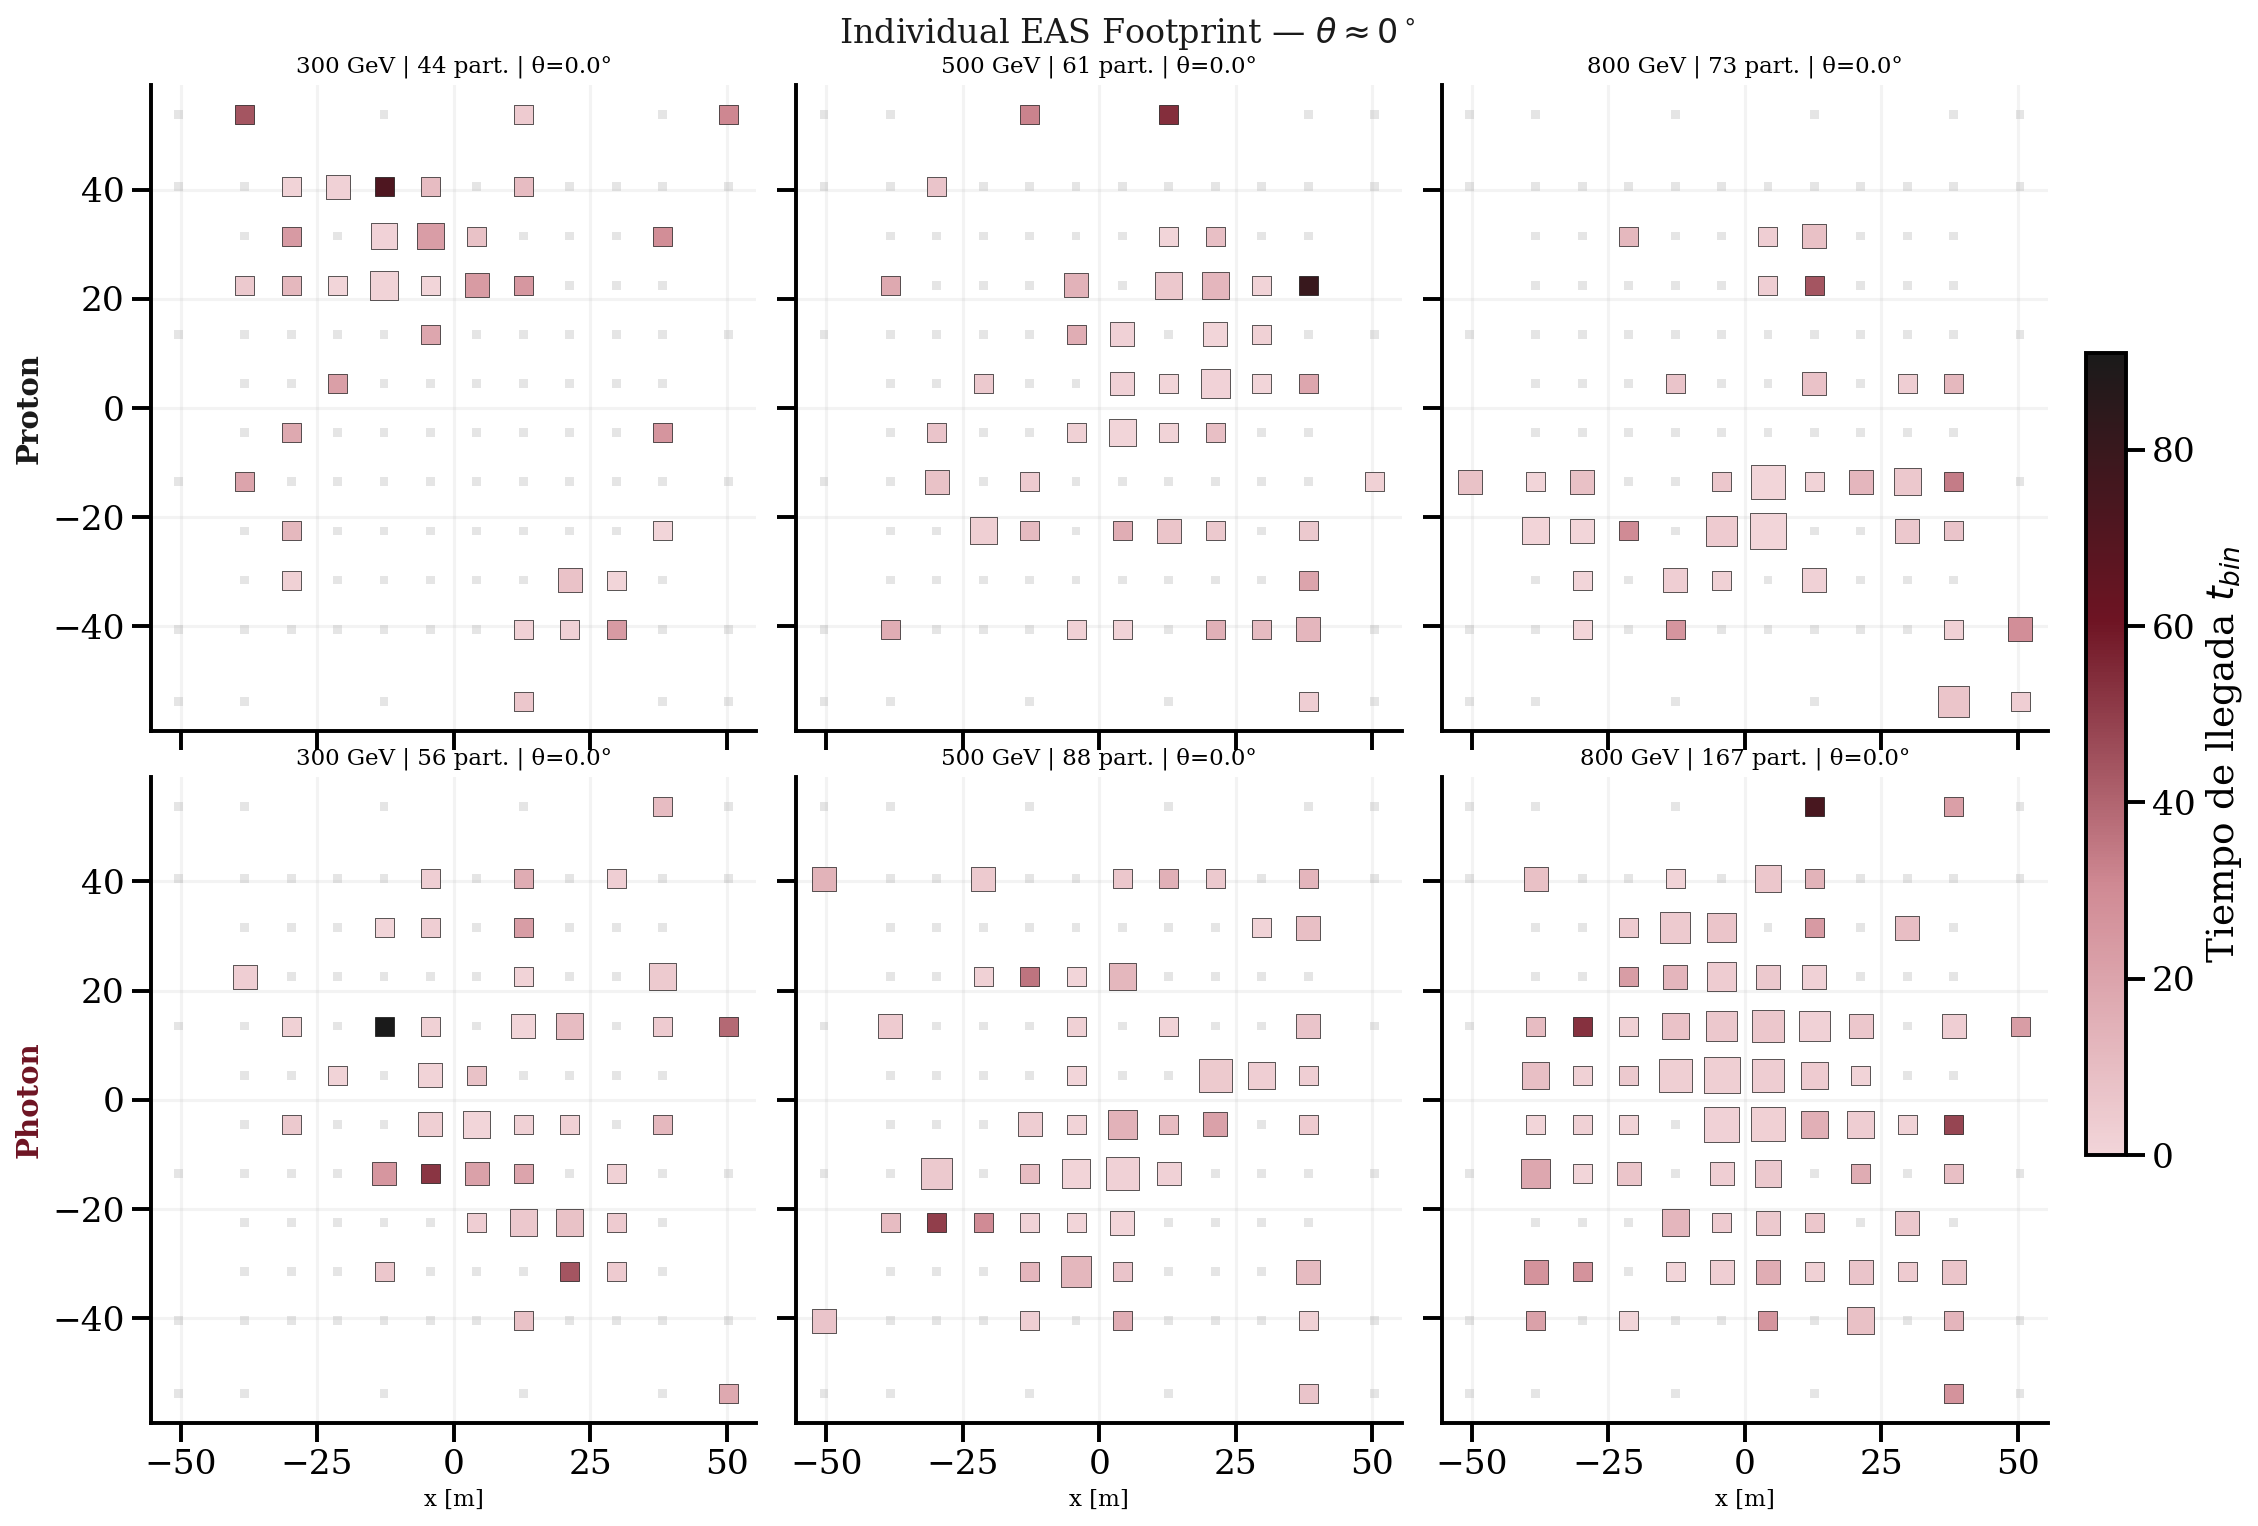
\includegraphics[width=1\linewidth]{figures/eas_individual_events.png}
    \caption[Representative individual EAS footprints by particle type and energy.]{Representative individual EAS footprints at $\theta \approx 0\degree$, for proton-induced (top row) and gamma-induced (bottom row) showers at 300, 500, and 800 GeV primary energy. Each event is selected as the one closest to the median total particle count for its group. Color encodes the arrival time $t_\mathrm{bin}$ of particles at each detector; marker size is proportional to particle count. Individual events exhibit significant stochastic fluctuations in lateral spread and hit multiplicity.}
    \label{fig:individual_events}
\end{figure}

Averaging over many events per bin removes this variability and exposes the underlying morphology. Figure~\ref{fig:footprint_grid} shows the mean footprints computed over roughly 770 events per cell: gamma-induced showers concentrate the deposited energy in a compact central core, whereas proton-induced showers spread it more widely and irregularly across the array. This morphological asymmetry is the primary discriminant the classification head learns to exploit.

\begin{figure}[!ht]
    \centering
    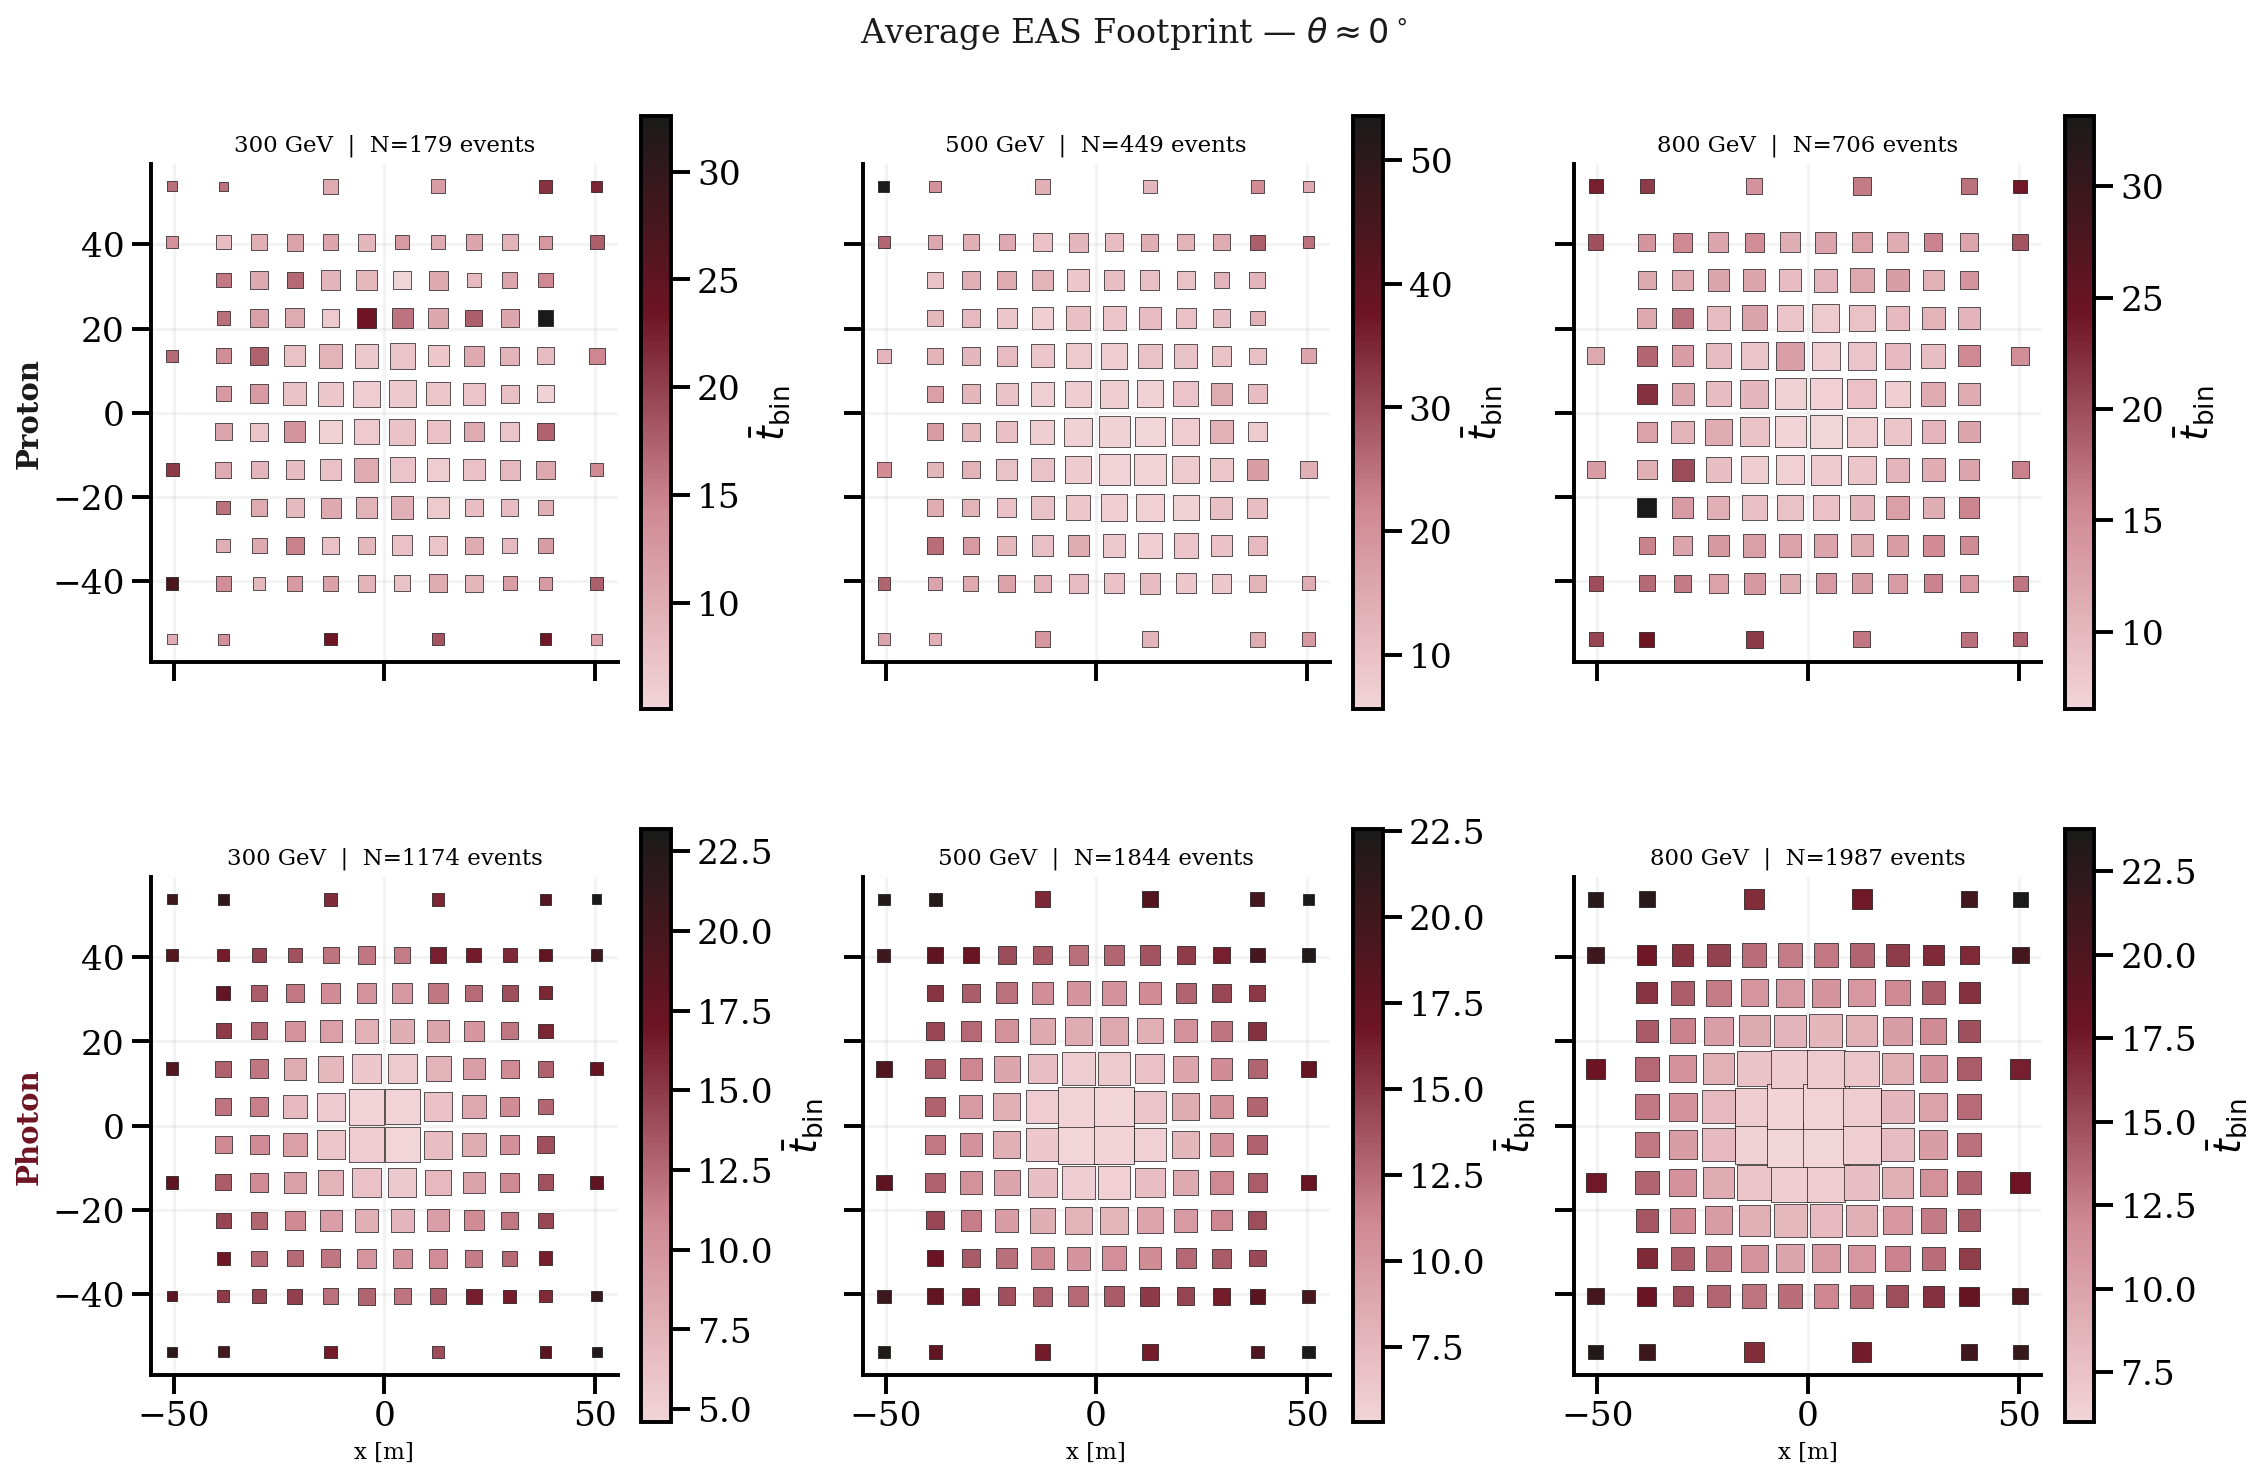
\includegraphics[width=1\linewidth]{figures/eas_footprint_grid.png}
    \caption[Average EAS footprints by particle type and energy.]{Average EAS footprints at $\theta \approx 0\degree$, computed over all events in each particle-type and energy bin (${\sim}770$ events per cell). Averaging suppresses single-event fluctuations and reveals the systematic morphological signatures of each class: gamma-induced showers produce a more compact, centrally concentrated deposit, while proton-induced showers exhibit a broader lateral spread and higher peripheral particle counts. Color encodes the mean arrival time $\bar{t}_\mathrm{bin}$; marker size is proportional to mean particle count.}
    \label{fig:footprint_grid}
\end{figure}

Both input branches are normalized before training. The sequential features are standardized channel-wise using the mean and standard deviation computed over the training set, and the global features are scaled to the unit interval using training set minimum and maximum values. Normalization statistics are computed exclusively on the training partition and applied without modification to the validation and test sets, ensuring that no information from the evaluation data influences the preprocessing.

\section{Data Stratification and Balance Strategy}

The raw simulated dataset is not uniformly distributed across the space of primary particle types, energies, and zenith angles. This imbalance arises from the interaction between the simulation configuration and the multiplicity filter: showers at large zenith angles or low energies produce fewer secondary particles at detector level on average and are therefore more frequently discarded. Left uncorrected, this imbalance would bias the shared encoder toward the conditions most heavily represented in the training data, degrading performance on underrepresented configurations and compromising the fairness of the multi-task optimization.
To address this, a stratified resampling procedure is applied before the dataset split. Let
\begin{equation}
    S = \{s_1, s_2, \ldots, s_K\}
\end{equation}
denote the set of all $K$ strata, where each stratum $s_i$ is defined by a unique combination of primary energy $E \in \{300,500,800\}$ GeV, particle type $p \in \{\text{proton}, \gamma\}$, and discretized zenith angle bin $\theta$. For each stratum $s_i$, let $n_i$ denote its event count after multiplicity filtering. The target population size is defined as
\begin{equation}
    n_\text{target} = \text{median}(\{n_1, n_2, \ldots, n_K\})
\end{equation}
which evaluates to $n_\text{target} = 593$ for this dataset. The median is preferred over the mean as a balancing objective because it is insensitive to outliers and extreme population disparities: under the median criterion, half of the strata are downsampled and half are upsampled, without being influenced by extremely large or small strata. The resampling procedure operates independently on each stratum:
\begin{equation}
n_i^{\text{balanced}} = \begin{cases}
\text{undersample}(s_i, n_{\text{target}}) & \text{if } n_i > n_{\text{target}} \\
\text{oversample}(s_i, n_{\text{target}}) & \text{if } n_i < n_{\text{target}} \\
n_i & \text{if } n_i = n_{\text{target}}
\end{cases}
\end{equation}

where undersampling randomly selects $n_{\text{target}}$ events from the $n_i$ available events without replacement, effectively removing $n_i - n_{\text{target}}$ events. Oversampling duplicates events with replacement until the stratum size reaches $n_{\text{target}}$, introducing $n_{\text{target}} - n_i$ duplicate samples. This ensures that after resampling, all strata satisfy $n_i^{\text{balanced}} = n_{\text{target}}$.

The resulting balanced dataset contains approximately 74,700 events in total. These are split into training, validation, and test partitions in a ratio of approximately 70:15:15, yielding roughly 52,300 training events, 11,200 validation events, and 11,200 test events. The split is performed after stratified resampling and maintains the balanced distribution across all three partitions. No event appears in more than one partition, and the test set is held out entirely until final evaluation. Figure~\ref{fig:data_balancing} illustrates the original event distributions per energy and the resampling target, and Table~\ref{tab:dataset_balancing} summarizes the dataset composition before and after balancing.
\begin{table}[ht!]
\centering
\caption[Dataset composition before and after balancing.]{Dataset composition before and after balancing. $\gamma$: \# gamma events, \textbf{p}: $\#$ proton events.}
\label{tab:dataset_balancing}
\begin{tabular}{cccc}
\toprule
\textbf{E (GeV)} & \textbf{$\gamma$} & \textbf{p} & \textbf{Total} \\
\midrule
\multicolumn{4}{c}{\textit{Original}} \\
300  & 14474 & 1958 & \textbf{16432} \\
500  & 27611 & 5306 & \textbf{32917} \\
800 & 36143 & 11496 & \textbf{47639} \\
\midrule
\multicolumn{4}{c}{\textit{Balanced}} \\
300  & 12453 & 12453 & \textbf{24906} \\
500  & 12453 & 12453 & \textbf{24906} \\
800  & 12453 & 12453 & \textbf{24906} \\
\bottomrule
\end{tabular}
\end{table}

Figure~\ref{fig:data_balancing} illustrates the effect of the resampling strategy across the three marginal distributions. After balancing, the label distribution is equalised between proton and gamma classes, the zenith angle distribution becomes uniform across the full $0\degree$--$40\degree$ range, and the energy distribution is balanced across the three primary energy levels. The resulting dataset satisfies $n_i^{\text{balanced}} = n_{\text{target}}$ for all $i \in \{1, \ldots, K\}$, ensuring equitable representation across all physics configurations.

\begin{figure*}[ht!]
    \centering
    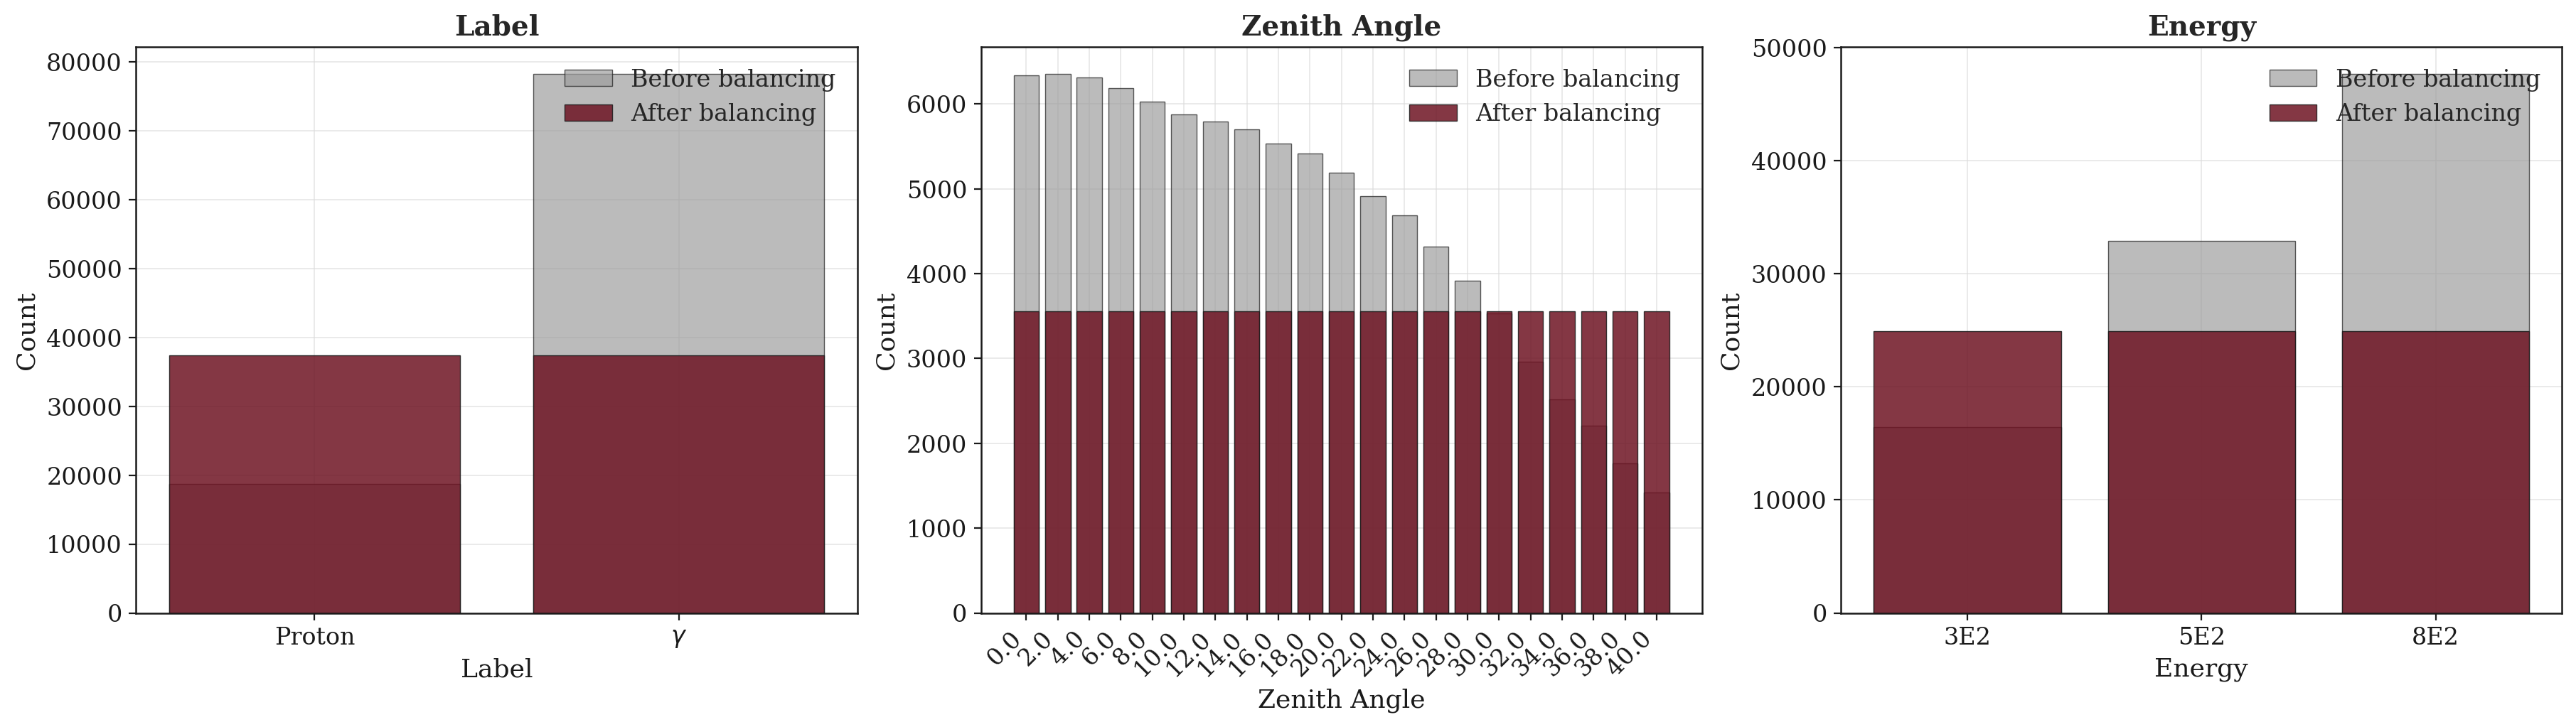
\includegraphics[width=1\linewidth]{figures/data_balancing.png}
    \caption[Event distributions before and after stratified balancing.]{Distribution of events by label, zenith angle, and primary energy before (grey) and after (dark red) stratified balancing. Grey bars extending above the dark red bars indicate categories that were undersampled to reach the median target of 593 events per stratum; categories where both bars align were already close to the target or were oversampled.}
    \label{fig:data_balancing}
\end{figure*}

This combined over- and undersampling approach ensures that each physics configuration is represented equitably during training. The final balanced dataset, whose composition by energy and particle type is summarized in Table~\ref{tab:dataset_split}, helps the model to develop unbiased decision boundaries across the entire parameter space.

\begin{table}[ht!]
\centering
\caption[Dataset composition after stratified balancing.]{Dataset composition after stratified balancing, showing the number of events by primary energy, particle type, and split. Energy labels: 3E2 = 300 GeV, 5E2 = 500 GeV, 8E2 = 800 GeV.}
\label{tab:dataset_split}
\begin{tabular}{lrrrrrrc}
\toprule
\textbf{Split} & \textbf{3E2-$\gamma$} & \textbf{3E2-p} & \textbf{5E2-$\gamma$} & \textbf{5E2-p} & \textbf{8E2-$\gamma$} & \textbf{8E2-p} & \textbf{Total} \\
\midrule
\textbf{Train}      & 8678 & 8684 & 8728 & 8718 & 8745 & 8749 & \textbf{52302} \\
\textbf{Val} & 1892 & 1894 & 1838 & 1875 & 1872 & 1836 & \textbf{11207} \\
\textbf{Test}       & 1883 & 1875 & 1887 & 1860 & 1836 & 1868 & \textbf{11209} \\
\bottomrule
\end{tabular}
\end{table}

A methodological note on the interaction between oversampling and the data split is warranted. Because the resampling procedure is applied before the split into training, validation, and test partitions, oversampled strata contain duplicated events. The splitting procedure assigns each event instance to exactly one partition, but for strata where $n_i < n_\text{target}$, different copies of the same physical event may appear in different partitions, creating a potential information leak between training and test data.

The magnitude of this effect is not negligible and is strongly class-dependent. As shown in Table~\ref{tab:dataset_balancing}, the gamma class is abundant at all three energies (78,228 events before balancing) and is therefore downsampled in every stratum, so all gamma events in the balanced dataset are unique. The proton class, by contrast, is scarce (18,760 events before balancing) and falls below the median target in every stratum, so all proton strata are oversampled. Consequently the balanced dataset contains $37{,}359 - 18{,}760 = 18{,}599$ duplicated proton instances, which amounts to roughly 25\% of the total dataset and approximately half of the proton class. Duplicate copies of a given proton event are distributed across the partitions, so a proton event in the test set frequently has an identical copy in the training set.

This asymmetry has a concrete implication for interpretation: it can selectively inflate the apparent performance on proton events. In particular, the markedly better energy resolution obtained for protons (16--18\%) compared to gammas (28--41\%, Section~\ref{subsec:energy}) is attributed below to shower physics, but a fraction of the gap could also reflect partial memorization of duplicated proton events. The gamma-class metrics are not subject to this effect, since gamma events are never duplicated. This caveat should be kept in mind when reading the per-class results. Alternative strategies that avoid the leak entirely --- performing the split before resampling, undersampling instead of oversampling, or replacing duplication with class-weighted losses or post-split augmentation --- would remove this ambiguity and represent a natural direction for future refinement.

\section{Model Architecture}

The reconstruction model is a hybrid CNN-Transformer architecture designed for multi-task learning over dual-input shower data. Its design reflects three requirements: the ability to extract local temporal features from the sequential input, the ability to model global dependencies across the full hit sequence, and the flexibility to specialize independently for each of the three reconstruction tasks without forcing a single shared representation to serve all objectives equally. A schematic diagram of the full architecture is shown in Figure~\ref{fig:flowchart}.

\textbf{CNN backbone.} The sequential input is first processed by a convolutional backbone consisting of three successive Conv1D layers, each with 128 filters, kernel size 7, same-padding, and ELU activation. Batch normalization is applied after each convolutional layer. After the third convolutional layer, a single max-pooling operation with stride 2 halves the temporal resolution before the representation is passed to the projection layers. The three-layer structure progressively expands the effective receptive field: the first layer captures local patterns within a handful of consecutive hits, while the third integrates information over a wider temporal window. The max-pooled output is then projected through three fully connected layers of dimensions 128, 256, and 128 with ELU activations, and dropout of rate 0.4 is applied after the 256-dimensional layer.

\textbf{Task-specific Transformer streams.} The architecture employs six independent Transformer streams, two per reconstruction task. For each task, one stream operates on the 128-dimensional CNN output sequence (the \textit{CNN stream}), and a second stream operates directly on the raw masked six-dimensional hit sequence (the \textit{RAW stream}). Each stream applies a single pre-norm Transformer encoder block with one attention head and key dimension $d_k = 32$, as described in Section~\ref{sec:transformer}. The CNN streams capture high-level temporal patterns abstracted by the convolutional backbone. The RAW streams attend directly to individual detector hits, enabling attention maps that can be interpreted in terms of specific physical observables, such as which detectors and time bins the model prioritizes for each task, without the indirection introduced by convolutional transformations. Using two dedicated streams per task ensures that each reconstruction objective can develop an independent attentional strategy without competing with the others for a shared mechanism.

\textbf{Fusion and output heads.} The output of each stream is summarized by global average pooling. For each task, the pooled CNN-stream vector (128 dimensions) and the pooled RAW-stream vector (6 dimensions, matching the raw feature depth) are concatenated to form a 134-dimensional fused attention representation, which is then concatenated with the five-dimensional global feature vector to yield a 139-dimensional fused representation. This representation is passed through a task-specific dense layer of 128 units with ELU activation and then mapped to the final prediction: a sigmoid-activated scalar for gamma-hadron classification and a linear-activated scalar for each regression task. Task-specific dropout is applied before the dense head, with rates of 0.35 for classification, no dropout for zenith angle regression, and 0.5 for energy estimation. The total model contains 531,375 parameters, of which 530,607 are trainable and 768 are non-trainable batch normalization statistics.

\clearpage
\begin{landscape}
    \centering
    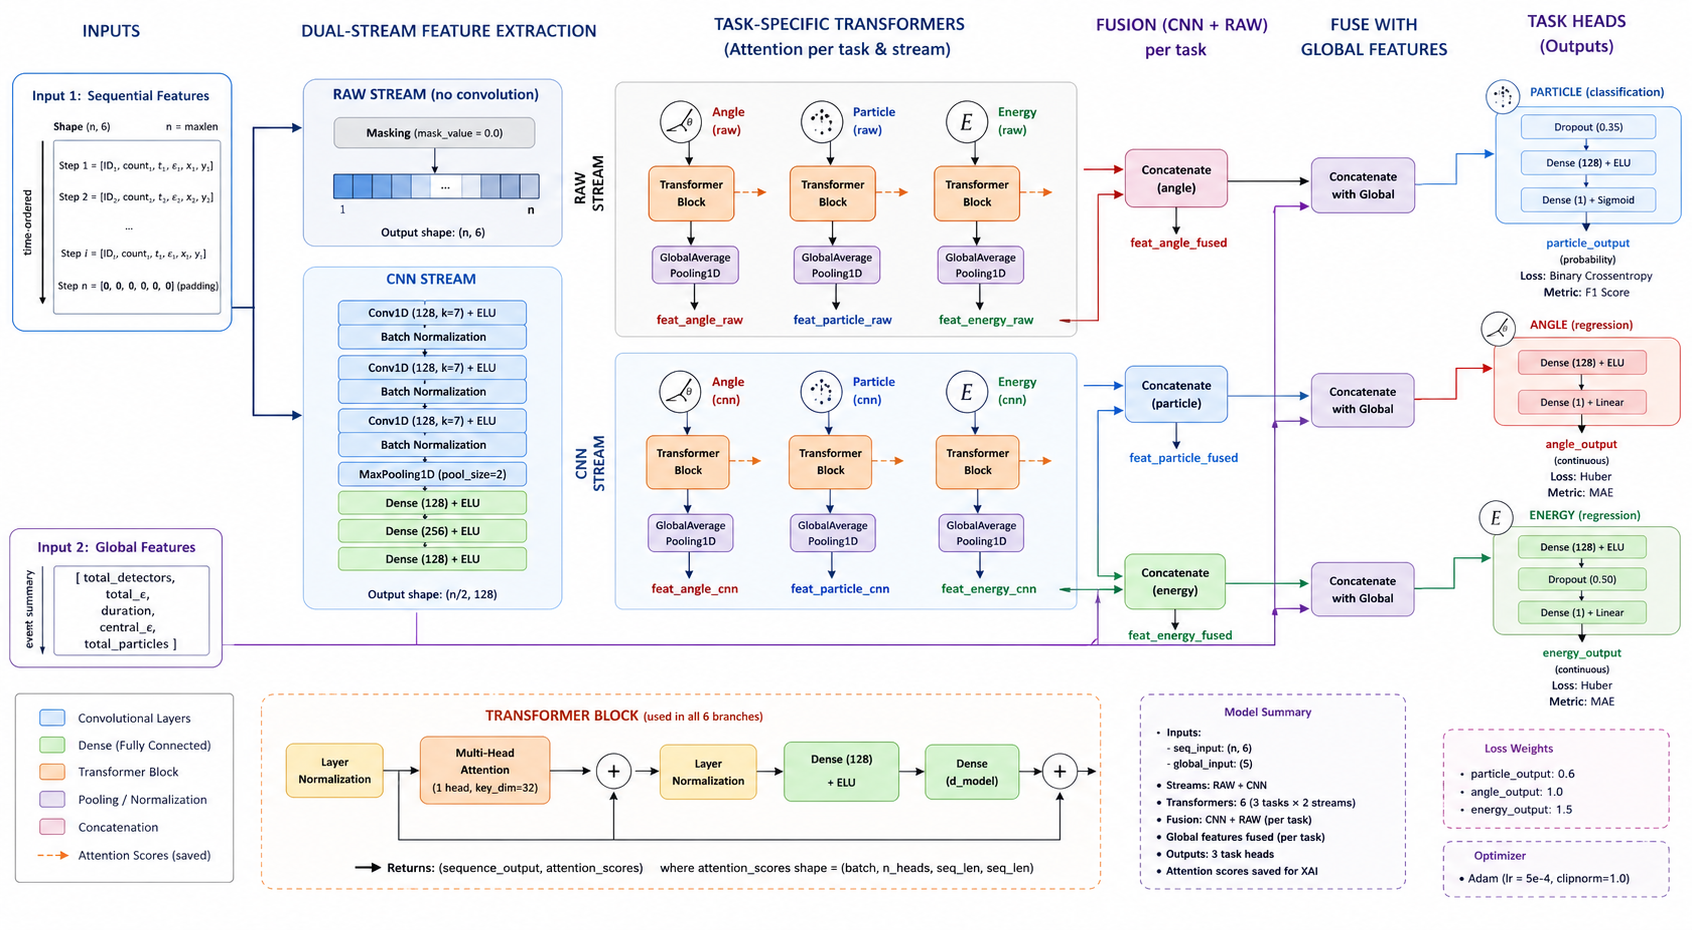
\includegraphics[width=\linewidth]{figures/flowchart_architecture.png}
    \captionof{figure}{Flow diagram of the CNN-Transformer multi-task model.}
    \label{fig:flowchart}
\end{landscape}
\clearpage

\section{Hyperparameter Optimization}
\label{sec:hyperparameter}

The model contains a number of hyperparameters that influence training dynamics and final performance, including the learning rate, task loss weights, and the dropout rates for the classification and energy heads. An initial search was conducted using Optuna~\shortcite{akiba2019optuna}, a framework for automated hyperparameter optimization based on Bayesian search with tree-structured Parzen estimators (TPE)~\shortcite{bergstra2011algorithms}. TPE models the distributions of hyperparameter configurations that lead to good and poor outcomes separately, and uses the ratio of these distributions to propose new trials that are more likely to improve the objective. This approach is substantially more sample-efficient than grid or random search, particularly when the hyperparameter space is high-dimensional.

The search space covered the learning rate over the range $[10^{-4}, 10^{-2}]$ on a logarithmic scale, the task loss weights $\lambda_\text{cls}$, $\lambda_\theta$, and $\lambda_E$ each over $[0.1, 2.0]$, and the dropout rates for the classification and energy heads independently over $[0.1, 0.6]$. Each trial trained the model for a fixed number of epochs and evaluated the combined validation loss as the optimization objective; divergent trials were pruned early using Optuna's built-in median pruner. The Optuna search provided initial estimates for the hyperparameter ranges, which were then refined through targeted manual tuning of the loss weights and dropout rates. The final configuration, reported in Table~\ref{tab:hyperparameters}, was selected based on validation performance across all three tasks simultaneously.

\begin{table}[htbp]
\centering
\caption[Consolidated hyperparameter configuration.]{Consolidated hyperparameter configuration for the final model.}
\label{tab:hyperparameters}
\footnotesize
\setlength{\tabcolsep}{7pt}
\renewcommand{\arraystretch}{1.1}
\begin{tabular}{llc}
\toprule
\textbf{Category} & \textbf{Parameter} & \textbf{Value} \\
\midrule
\multirow{3}{*}{CNN backbone}
  & Conv1D filters & 128 \\
  & Kernel size & 7 \\
  & CNN dropout & 0.4 \\
\midrule
\multirow{2}{*}{Transformer}
  & Attention heads & 1 \\
  & Key dimension $d_k$ & 32 \\
\midrule
\multirow{3}{*}{Task weights}
  & $\lambda_\text{cls}$ & 0.6 \\
  & $\lambda_\theta$ & 1.0 \\
  & $\lambda_E$ & 1.5 \\
\midrule
\multirow{3}{*}{Task dropout}
  & Classification & 0.35 \\
  & Angle & 0.0 \\
  & Energy & 0.5 \\
\midrule
\multirow{5}{*}{Training}
  & Optimizer & Adam \\
  & Learning rate & $5 \times 10^{-4}$ \\
  & Gradient clip norm & 1.0 \\
  & LR reduction patience & 7 epochs \\
  & Early stopping patience & 15 epochs \\
\midrule
\multirow{2}{*}{Data}
  & Batch size & 64 \\
  & Max sequence length & 472 \\
\bottomrule
\end{tabular}
\end{table}

The final task weights are
\begin{align*}
    \lambda_\text{cls} &= 0.6 \\
    \lambda_\theta &= 1.0 \\
    \lambda_E &= 1.5 ,
\end{align*}
reflecting the relative difficulty of each task and the need to prevent the binary classification objective from dominating the regression signals early in training.

\section{Training Configuration}

The model is trained by minimizing the weighted multi-task loss:
\begin{equation}
    \mathcal{L}_\text{total} = \lambda_\text{cls} \mathcal{L}_\text{cls} + \lambda_\theta \mathcal{L}_\theta + \lambda_E \mathcal{L}_E
\end{equation}
where $\mathcal{L}_\text{cls}$ is the binary cross-entropy loss for gamma-hadron classification and $\mathcal{L}_\theta$, $\mathcal{L}_E$ are Huber losses for zenith angle and energy regression respectively, as defined in Section~\ref{sec:multitask}. Optimization is performed using the Adam optimizer~\shortcite{kingma2015adam} with learning rate $5 \times 10^{-4}$ and gradient norm clipping at 1.0. The learning rate is reduced by a factor of 0.5 whenever the combined validation loss fails to improve for seven consecutive epochs, with a minimum learning rate floor of $10^{-6}$. This plateau reduction schedule allows the optimizer to take larger steps during the initial training phases and shift to finer adjustments as the model approaches convergence, which proved effective for balancing the three task objectives simultaneously.

Training is stopped early when the combined validation loss fails to improve for 15 consecutive epochs, and the model checkpoint achieving the lowest validation loss is restored for final evaluation. No information from the test set is used at any point during training or hyperparameter search. Table~\ref{tab:hyperparameters} consolidates all hyperparameters of the final configuration.

All experiments were conducted on a single NVIDIA GeForce RTX 3050 Ti Laptop GPU (4 GB VRAM) using TensorFlow 2.10 with CUDA 11.2. A full training run to convergence (61 epochs, with the best checkpoint at epoch 46) required approximately 45 minutes. The total model contains 531,375 parameters, of which 530,607 are trainable and 768 are non-trainable batch normalization statistics.
    
    % Chapter 4: Results and Explainability %
    \chapter{Results and Explainability}
\label{ch:results}

This chapter presents the evaluation of the CNN-Transformer model on the held-out test set, together with the full suite of explainability analyses and the detector robustness study. All results correspond to the six-stream architecture described in Chapter~\ref{ch:methodology}, which extends the three-stream CNN-Transformer model introduced in~\shortciteA{navarro2026transformer} with independent RAW attention streams per task, enabling attention maps at the level of individual detector hits. The test partition comprises 11,209 events and was withheld entirely during training and hyperparameter search. Section~\ref{sec:performance} reports quantitative performance across the three reconstruction tasks and compares them with the state of the art. Section~\ref{sec:explainability} presents two complementary feature importance analyses and the attention pattern study. Section~\ref{sec:robustness} quantifies model robustness to detector failures and derives first data-driven insights on array design.

% ============================================================
\section{Multi-Task Performance}
\label{sec:performance}
% ============================================================

Figure~\ref{fig:training_curves} shows the training and validation loss and metric curves across epochs. The model trained for 61 epochs before early stopping was triggered, with the best checkpoint at epoch 46 restored for evaluation. All three tasks converge jointly without any task dominating the optimization, and the gap between training and validation curves is narrow throughout, indicating that the regularization strategy is effective.

\begin{figure*}[ht!]
    \centering
    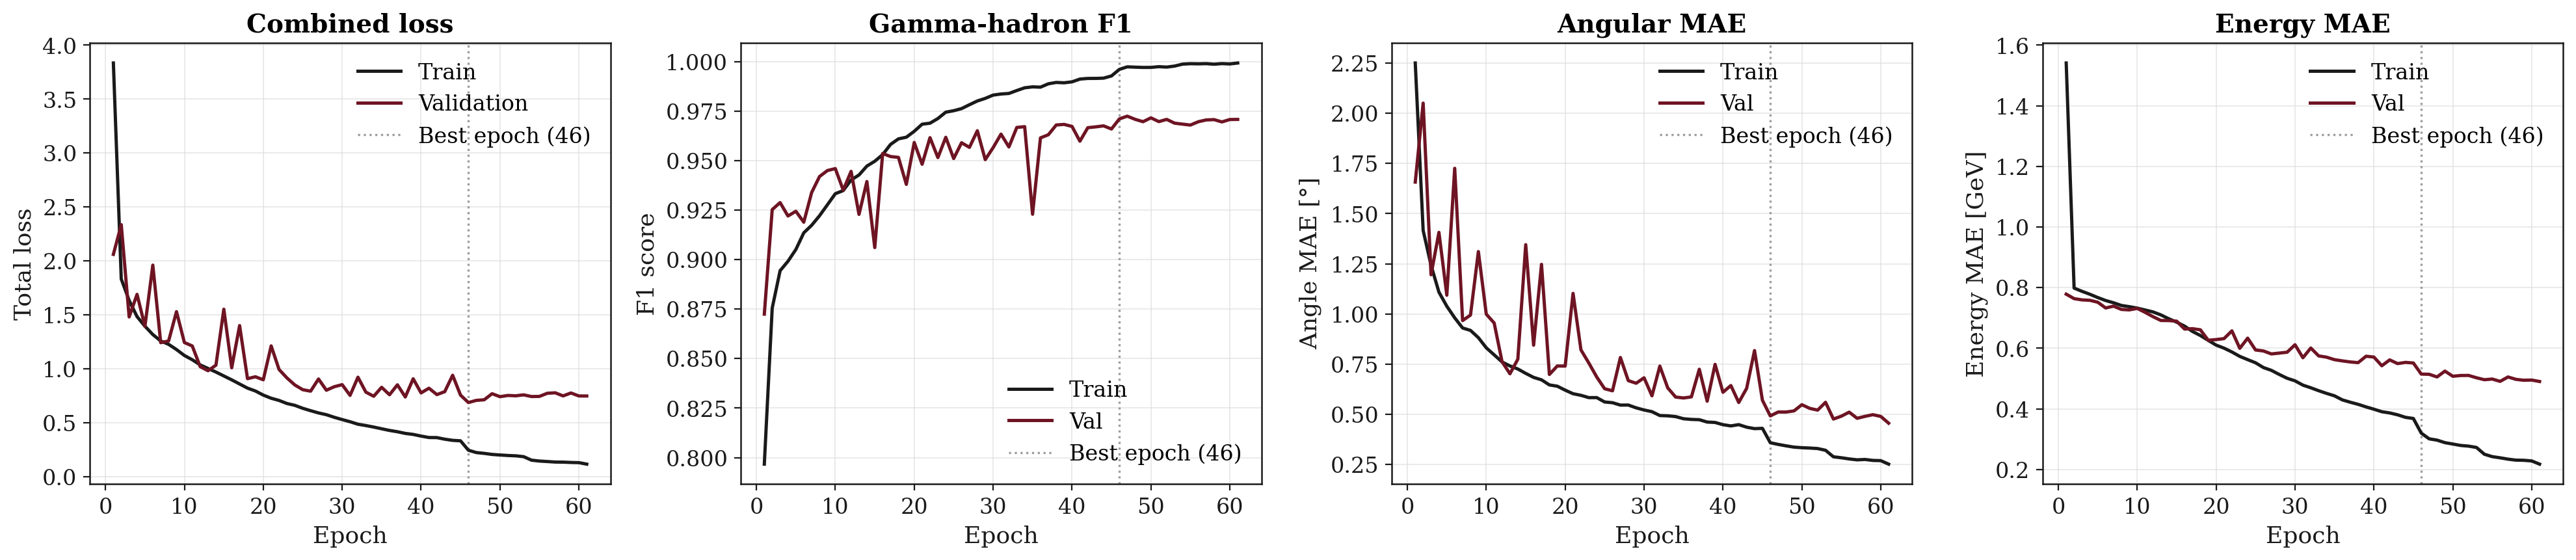
\includegraphics[width=1\linewidth]{figures/training_curves.png}
    \caption[Training and validation curves across the three tasks.]{Training and validation curves as a function of epoch. From left to right: combined multi-task loss, gamma-hadron F1 score, angular MAE, and energy MAE. The vertical dotted line in each panel marks the best checkpoint epoch (minimum combined validation loss), restored for the final evaluation. All tasks converge jointly without divergence.}
    \label{fig:training_curves}
\end{figure*}

A note on notation is in order before the results are presented. Throughout this chapter, a circumflex denotes a quantity predicted by the model and the subscript ``true'' denotes the corresponding Monte Carlo value: $\hat{\theta}$ and $\theta_\text{true}$ are the reconstructed and true zenith angles of an event, and $\hat{E}$ and $E_\text{true}$ its reconstructed and true primary energies. The \textit{angular residual} of an event is the difference $\hat{\theta} - \theta_\text{true}$, and its absolute value $|\hat{\theta} - \theta_\text{true}|$ is the absolute angular error.

Table~\ref{tab:performance_summary} provides a consolidated view of the primary metrics across all three tasks, including domain-specific figures of merit.

\begin{table}[ht!]
\centering
\caption[Summary of multi-task reconstruction performance.]{Summary of multi-task reconstruction performance on the test set, including domain-specific figures of merit. $Q = \varepsilon_\gamma / \sqrt{\varepsilon_p}$ is the quality factor for gamma-hadron separation, defined in full in Section~\ref{sec:apx_qfactor}. PSF$_{68}$ is the 68\% containment radius of the angular residual distribution, defined in full in Section~\ref{sec:apx_psf}.}
\label{tab:performance_summary}
\setlength{\tabcolsep}{8pt}
\renewcommand{\arraystretch}{1.2}
\begin{tabular}{lll}
\toprule
\textbf{Task} & \textbf{Primary Metric} & \textbf{Additional} \\
\midrule
Gamma-Hadron   & AUC = 0.991      & $Q$-factor = 5.48, $\varepsilon_\gamma = 0.971$ \\
Zenith Angle   & MAE = $0.484\degree$ & PSF$_{68}$ = $0.50\degree$, RMS = $0.74\degree$ \\
Energy         & MAE = 103.72 GeV & $\sigma_E / E$ = 33.1\%, $R^2$ = 0.453 \\
\bottomrule
\end{tabular}
\end{table}

\subsection{Gamma-Hadron Discrimination}
\label{subsec:particle}

Table~\ref{tab:particle_metrics} summarizes the classification performance on the test set. The model achieves an area under the receiver operating characteristic (ROC) curve (AUC) of 0.991, an F1-score of 0.970, and an overall accuracy of 96.99\%. The quality factor $Q = \varepsilon_\gamma / \sqrt{\varepsilon_p}$, a standard figure of merit in gamma-ray astronomy that quantifies signal-to-noise ratio, evaluates to $Q = 5.48$.

\begin{table}[ht!]
\centering
\caption[Gamma-hadron discrimination performance on the test set.]{Classification performance on the test set. Precision, recall, and F1-score are reported for each class. The test partition comprises 11,209 events, 5,606 proton-induced and 5,603 gamma-induced, so the two classes are balanced to within 0.03\%.}
\label{tab:particle_metrics}
\setlength{\tabcolsep}{9pt}
\renewcommand{\arraystretch}{1.15}
\begin{tabular}{lccc}
\toprule
\textbf{Class} & \textbf{Precision} & \textbf{Recall} & \textbf{F1} \\
\midrule
Proton   & 0.971 & 0.969 & 0.970 \\
$\gamma$ & 0.969 & 0.971 & 0.970 \\
\midrule
\textbf{Overall} & \multicolumn{3}{c}{Accuracy: \textbf{96.99\%} $\quad$ AUC: \textbf{0.991}} \\
\bottomrule
\end{tabular}
\end{table}

Figure~\ref{fig:particle_results} shows the row-normalized confusion matrix, with the raw event counts, and the ROC curve. Both classes are reconstructed with high fidelity: $96.9\%$ of proton events and $97.1\%$ of gamma events are classified correctly, and the ROC curve rises steeply to an AUC of $0.991$. The few percent of misclassified events correspond to the small overlap between the two classes near the decision threshold at $P(\gamma)=0.5$.

\begin{figure*}[ht!]
    \centering
    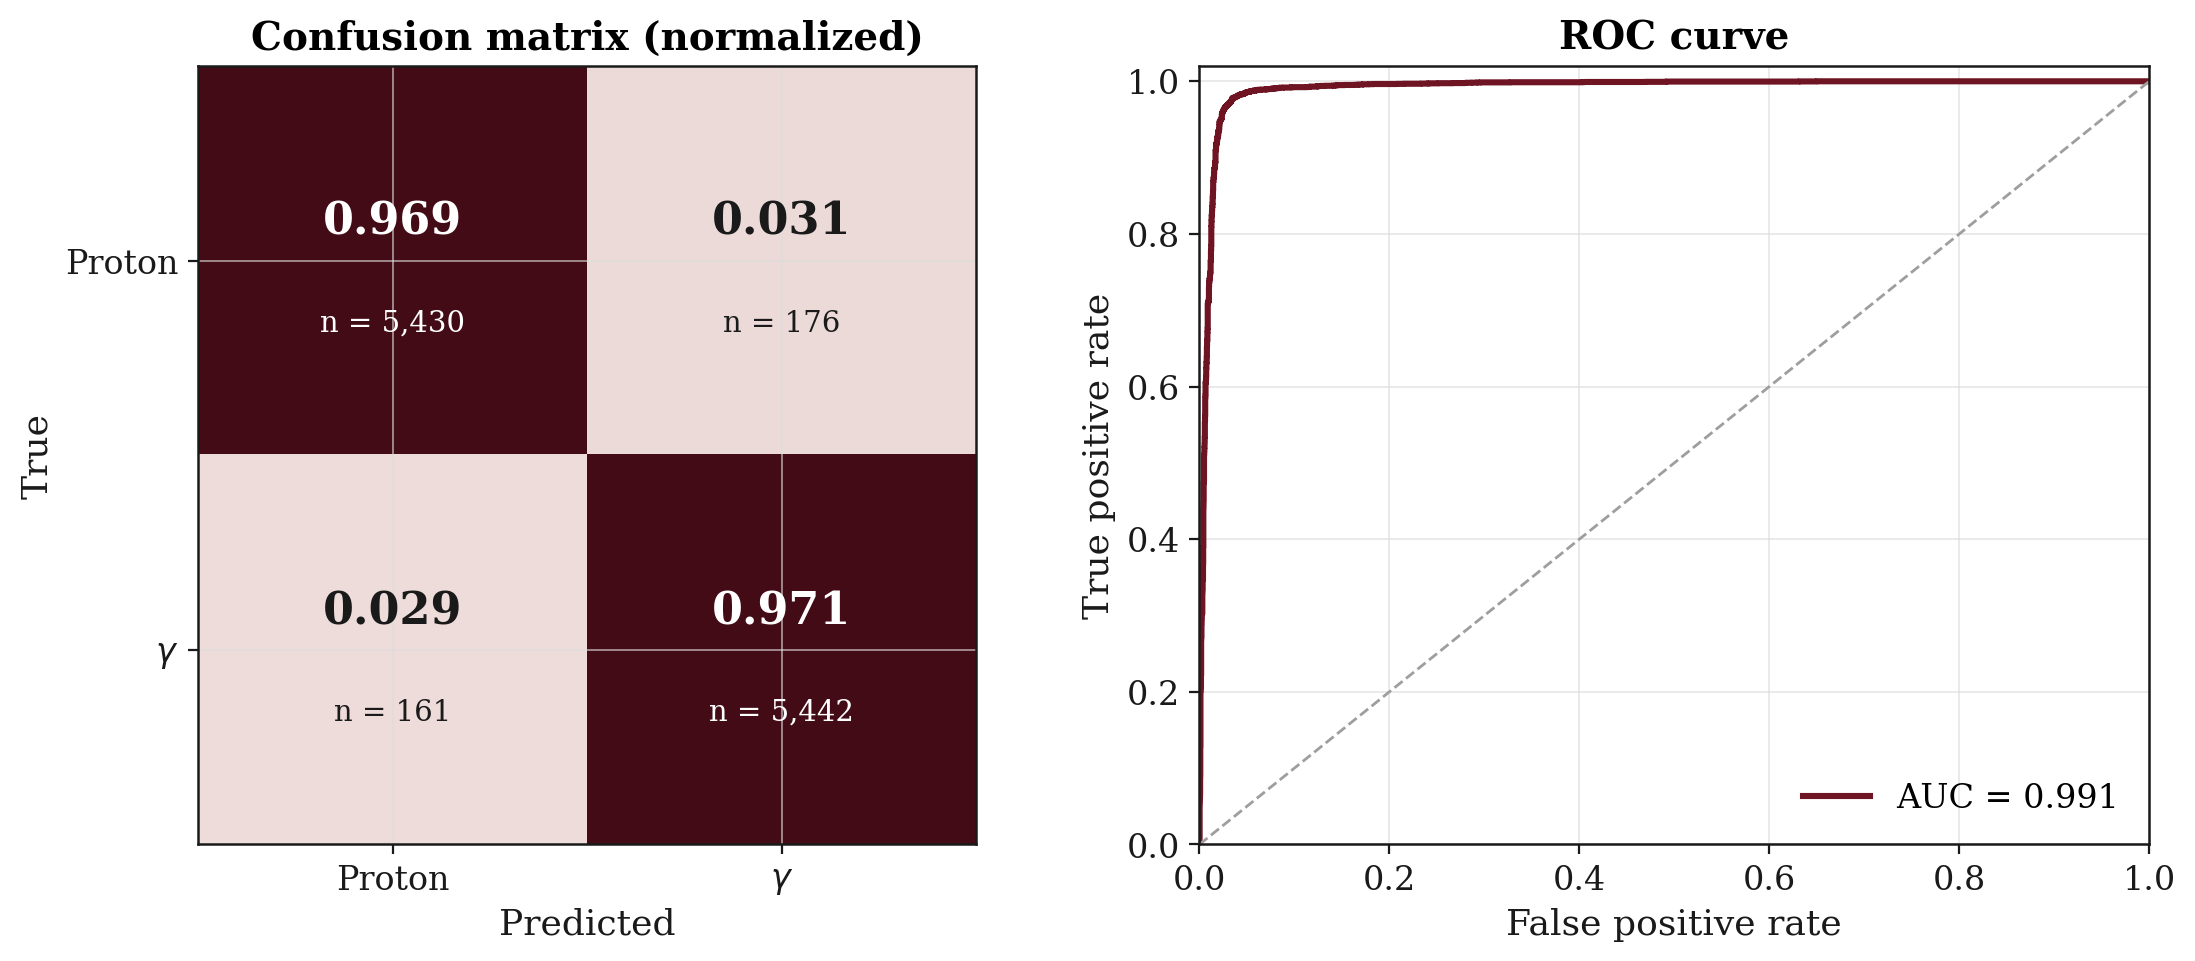
\includegraphics[width=1\linewidth]{figures/particle_results.png}
    \caption[Gamma-hadron discrimination results.]{Gamma-hadron discrimination on the test set. \textbf{Left:} row-normalized confusion matrix, with the raw event count shown below each fraction. \textbf{Right:} ROC curve (AUC = 0.991).}
    \label{fig:particle_results}
\end{figure*}

Figure~\ref{fig:roc_stratified} shows the ROC curves grouped by primary energy and by zenith angle bin: each curve is computed separately within the events sharing a given value of that variable, rather than over the test set as a whole, which isolates how discrimination depends on it. Discrimination improves at lower energies: the AUC is 0.998 at 300 GeV, 0.991 at 500 GeV, and 0.981 at 800 GeV.

This trend is physically consistent. At 300 GeV, electromagnetic showers are compact with a well-defined core signature, while hadronic showers at the same energy are sparse and noisy, making the morphological contrast between the two classes large. As the primary energy increases toward 800 GeV, both shower types develop larger and more complex footprints with greater stochastic fluctuations. In addition, a growing fraction of the energy of a hadronic shower is channelled into its electromagnetic component through neutral pion decay, the mechanism described in Section~\ref{subsec:hadronic_showers}. Hadronic events therefore acquire progressively more of the compact, centrally concentrated signature that distinguishes gamma-induced showers in the first place. Both effects reduce the morphological contrast between the two classes.

Across zenith angle bins the AUC ranges from 0.984 to 0.994, so discrimination is essentially independent of shower inclination over the range covered by the training data.

\begin{figure}[ht!]
    \centering
    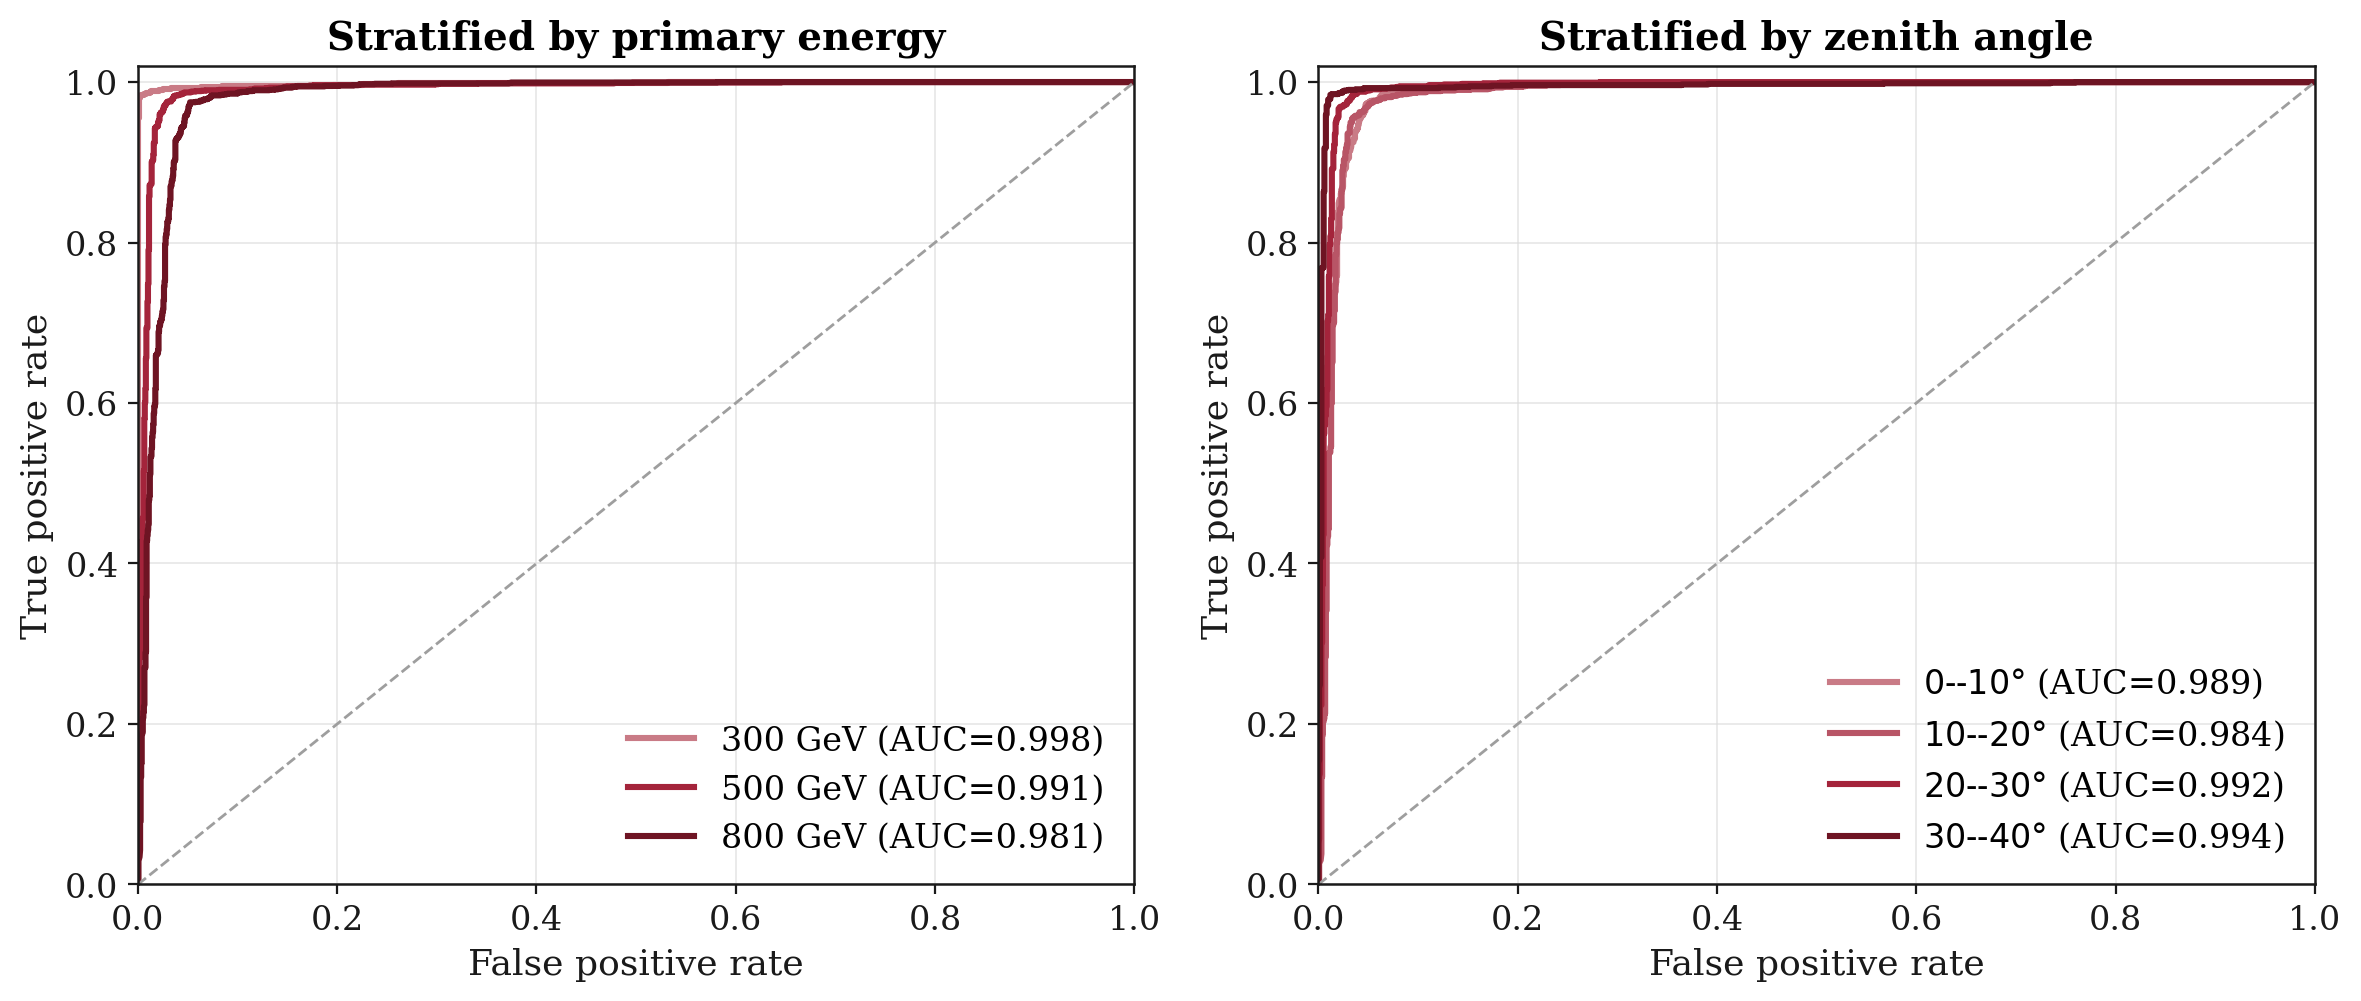
\includegraphics[width=0.85\linewidth]{figures/roc_stratified.png}
    \caption[ROC curves grouped by energy and zenith angle.]{ROC curves for gamma-hadron discrimination, grouped by primary energy (left) and zenith angle bin (right). AUC values are shown in the legend for each group.}
    \label{fig:roc_stratified}
\end{figure}

\subsection{Zenith Angle Reconstruction}
\label{subsec:angle}

The model achieves a mean absolute error of $\text{MAE}_\theta = 0.484\degree$ on the test set, with a coefficient of determination $R^2 = 0.996$. These results represent a significant improvement over both the traditional reconstruction baseline for CONDOR reported in~\shortciteA{arratia2025condor} (approximately 1--2\degree) and the predecessor CNN-LSTM model of~\shortciteA{navarro2025multi} ($\text{MAE}_\theta = 1.14\degree$). Table~\ref{tab:angle_metrics} summarizes the angular resolution metrics.

\begin{table}[ht!]
\centering
\caption[Zenith angle reconstruction metrics on the test set.]{Zenith angle reconstruction performance on the test set.}
\label{tab:angle_metrics}
\setlength{\tabcolsep}{11pt}
\renewcommand{\arraystretch}{1.15}
\begin{tabular}{lc}
\toprule
\textbf{Metric} & \textbf{Value} \\
\midrule
MAE            & $0.484\degree$ \\
RMSE           & $0.736\degree$ \\
$R^2$          & 0.996 \\
\bottomrule
\end{tabular}
\end{table}

Figure~\ref{fig:angle_results} shows the absolute and relative error distributions by particle type, together with the linearity profile $\mathbb{E}[\hat{\theta}\,|\,\theta_\text{true}]$. The absolute error distribution is heavily concentrated below $1\degree$ for both particle types, with a mean bias of $+0.036\degree$, confirming that the model is nearly unbiased across the range. Events with $\theta_\text{true} = 0\degree$ are excluded from the relative error panel, as the fractional residual $(\hat{\theta} - \theta_\text{true})/\theta_\text{true}$ is undefined at the origin. The linearity profile follows the ideal diagonal closely, with residuals that are symmetric and stable from $0\degree$ to $40\degree$.

\begin{figure*}[ht!]
    \centering
    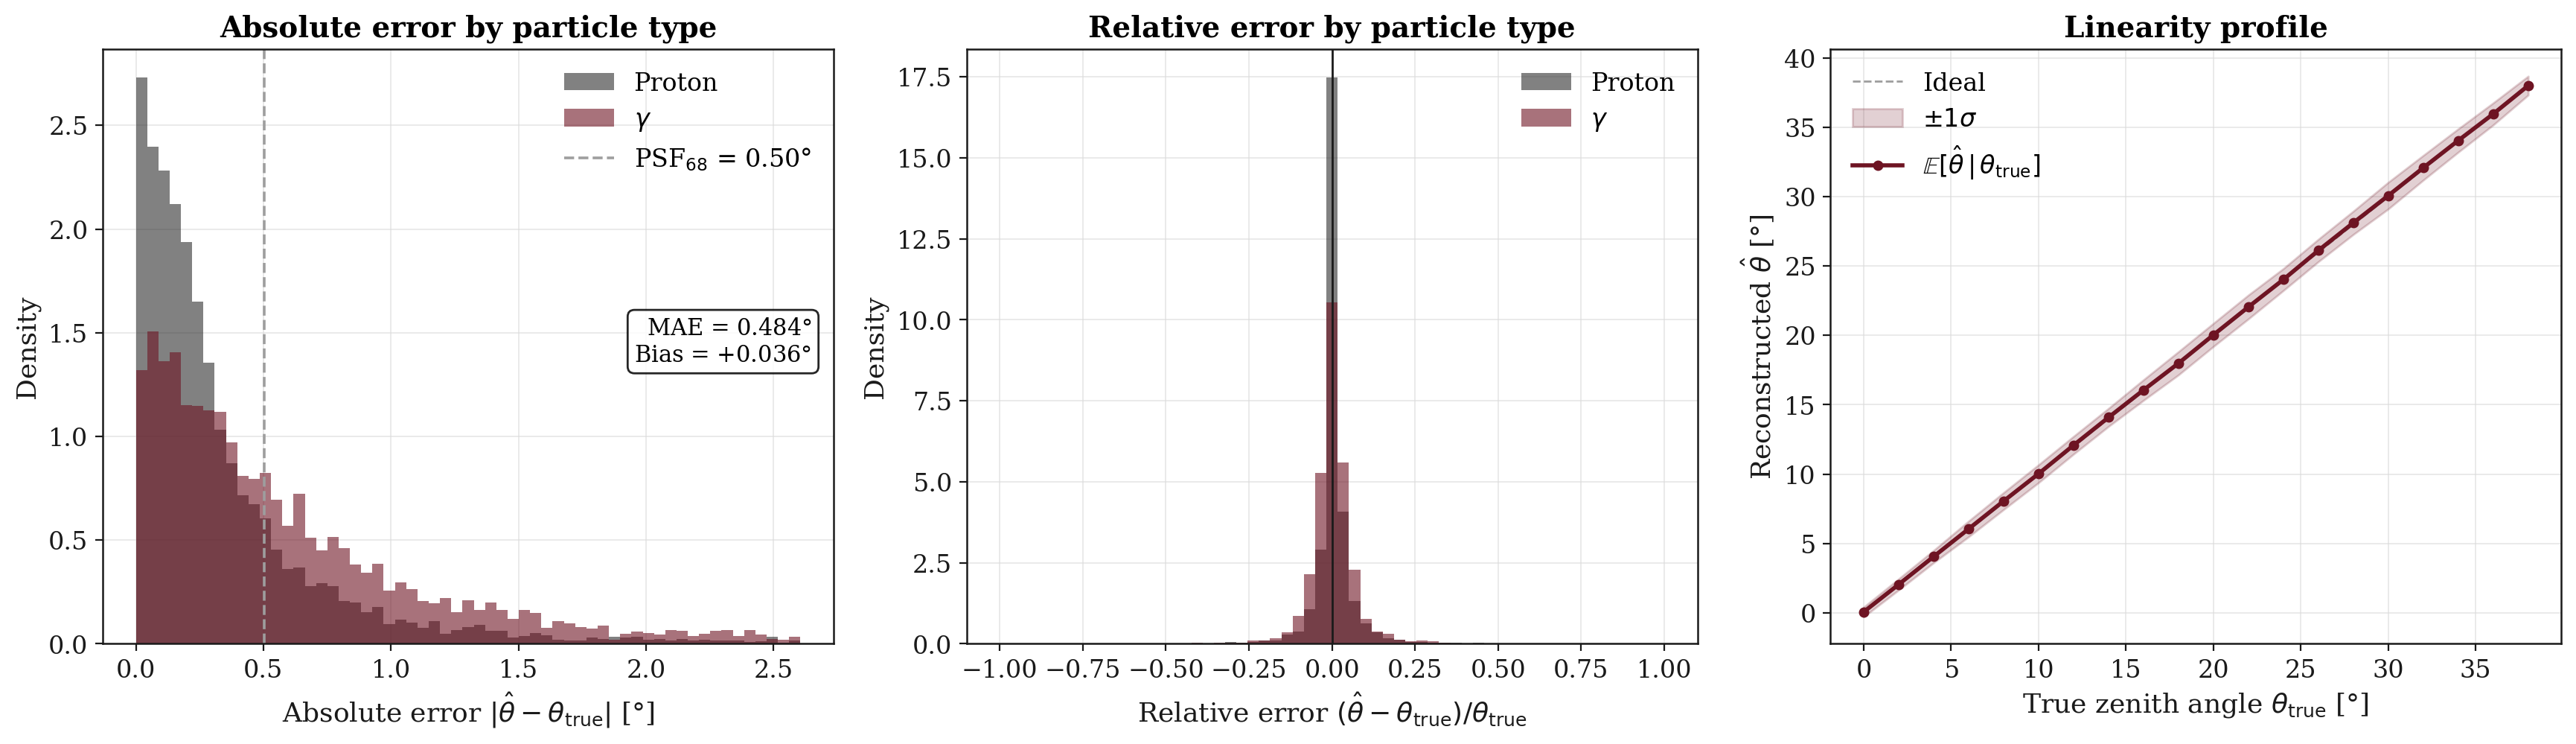
\includegraphics[width=1\linewidth]{figures/angle_results.png}
    \caption[Zenith angle reconstruction results.]{Zenith angle reconstruction on the test set. \textbf{Left:} distribution of the absolute error $|\hat{\theta}-\theta_\text{true}|$ for proton and gamma events, with key metrics inset. \textbf{Center:} relative error distribution $(\hat{\theta}-\theta_\text{true})/\theta_\text{true}$ by particle type. \textbf{Right:} mean reconstructed angle $\mathbb{E}[\hat{\theta}\,|\,\theta_\text{true}]$ with $\pm 1\sigma$ bands, confirming linearity across the full $0\degree$--$40\degree$ range.}
    \label{fig:angle_results}
\end{figure*}

The MAE of $0.484\degree$ corresponds to sub-degree pointing accuracy. The 68\% containment radius of the angular residual distribution, PSF$_{68} = 0.50\degree$, is the standard figure of merit for source identification in gamma-ray astronomy. The RMSE-to-MAE ratio of 1.52 is moderately above the value expected for a pure Gaussian residual distribution ($\sqrt{\pi/2} \approx 1.25$), indicating mildly heavier-than-Gaussian tails; large outlier reconstructions are present but infrequent. Performance is stable across the full $0\degree$--$40\degree$ zenith range covered by the training data.

\subsection{Energy Estimation}
\label{subsec:energy}

Energy estimation is the most challenging of the three tasks due to the discrete and narrow primary energy range (300--800 GeV). The model achieves $\text{MAE}_E = 103.72$ GeV and $\text{RMSE}_E = 151.80$ GeV on the test set, with an overall fractional energy resolution $\sigma_E/E = 33.1\%$ and $R^2 = 0.453$. The stratified analysis in Table~\ref{tab:energy_stratified} shows that the resolution varies substantially by particle type and energy, ranging from 16--20\% for protons across all energy bins to 45\% for gamma events at 300 GeV. The low $R^2$ reflects the discrete nature of the three training energies rather than a modeling failure: the coefficient of determination penalizes the large inter-class variance that dominates when only three energy values are present. Table~\ref{tab:energy_metrics} summarizes the scalar metrics.

\begin{table}[ht!]
\centering
\caption[Energy estimation metrics on the test set.]{Energy estimation performance on the test set.}
\label{tab:energy_metrics}
\setlength{\tabcolsep}{11pt}
\renewcommand{\arraystretch}{1.15}
\begin{tabular}{lc}
\toprule
\textbf{Metric} & \textbf{Value} \\
\midrule
MAE  & 103.72 GeV \\
RMSE & 151.80 GeV \\
Pull $\sigma$ & 0.331 \\
\bottomrule
\end{tabular}
\end{table}

The bias analysis reveals a systematic energy-dependent trend, summarized in Table~\ref{tab:energy_stratified}: the model overestimates at 300 GeV and underestimates at 800 GeV, with the effect more pronounced for gamma events than for protons. This is a consequence of the discrete training energies combined with shower fluctuations. At 300 GeV, electromagnetic showers can occasionally develop late, producing a footprint more typical of a higher-energy event; at 800 GeV, shower fluctuations in the opposite direction cause the model to pull predictions toward the center of the energy range. This regression-toward-the-mean bias is expected for discrete-target regression and should be accounted for when applying the model to analysis pipelines.

\begin{table}[ht!]
\centering
\caption[Energy bias and resolution split by particle type.]{Energy bias and resolution per true energy bin, split by particle type. Bias = mean fractional deviation $(\hat{E}-E)/E$; Resolution = standard deviation of the fractional residual. Both expressed as percentages.}
\label{tab:energy_stratified}
\setlength{\tabcolsep}{8pt}
\renewcommand{\arraystretch}{1.2}
\begin{tabular}{lccccc}
\toprule
 & \multicolumn{2}{c}{\textbf{Proton}} & & \multicolumn{2}{c}{\textbf{Gamma}} \\
\cmidrule{2-3} \cmidrule{5-6}
\textbf{Energy} & Bias (\%) & Res. (\%) & & Bias (\%) & Res. (\%) \\
\midrule
300 GeV & $+6.0$  & 20.2 & & $+43.8$ & 45.3 \\
500 GeV & $+6.0$  & 19.9 & & $+12.0$ & 29.2 \\
800 GeV & $-11.2$ & 15.5 & & $-17.7$ & 17.5 \\
\bottomrule
\end{tabular}
\end{table}

Figure~\ref{fig:energy_analysis} shows the overall pull distribution and its decomposition by particle type. The overall pull is approximately Gaussian with $\mu = 0.065$ and $\sigma = 0.331$; the small positive mean indicates a systematic overestimation of approximately $6.5\%$, consistent with the regression-toward-the-mean effect identified in the stratified analysis: the model pulls extreme predictions toward the center of the training energy range. The per-class pull distributions confirm the same class asymmetry visible in Table~\ref{tab:energy_stratified}: proton events have a substantially narrower pull ($\sigma_p \approx 0.20$) than gamma events ($\sigma_\gamma \approx 0.41$). Proton-induced showers spread over many detectors with a stable lateral profile at fixed energy, whereas gamma-induced showers depend more sensitively on the electromagnetic-core position within the array, which is a larger source of variance for energy inference. Proton events are essentially unbiased ($\mu_p \approx 0.004$), while the overall positive mean of the combined distribution is driven primarily by a $\sim 13\%$ overestimate in the gamma class ($\mu_\gamma \approx 0.13$).

\begin{figure*}[ht!]
    \centering
    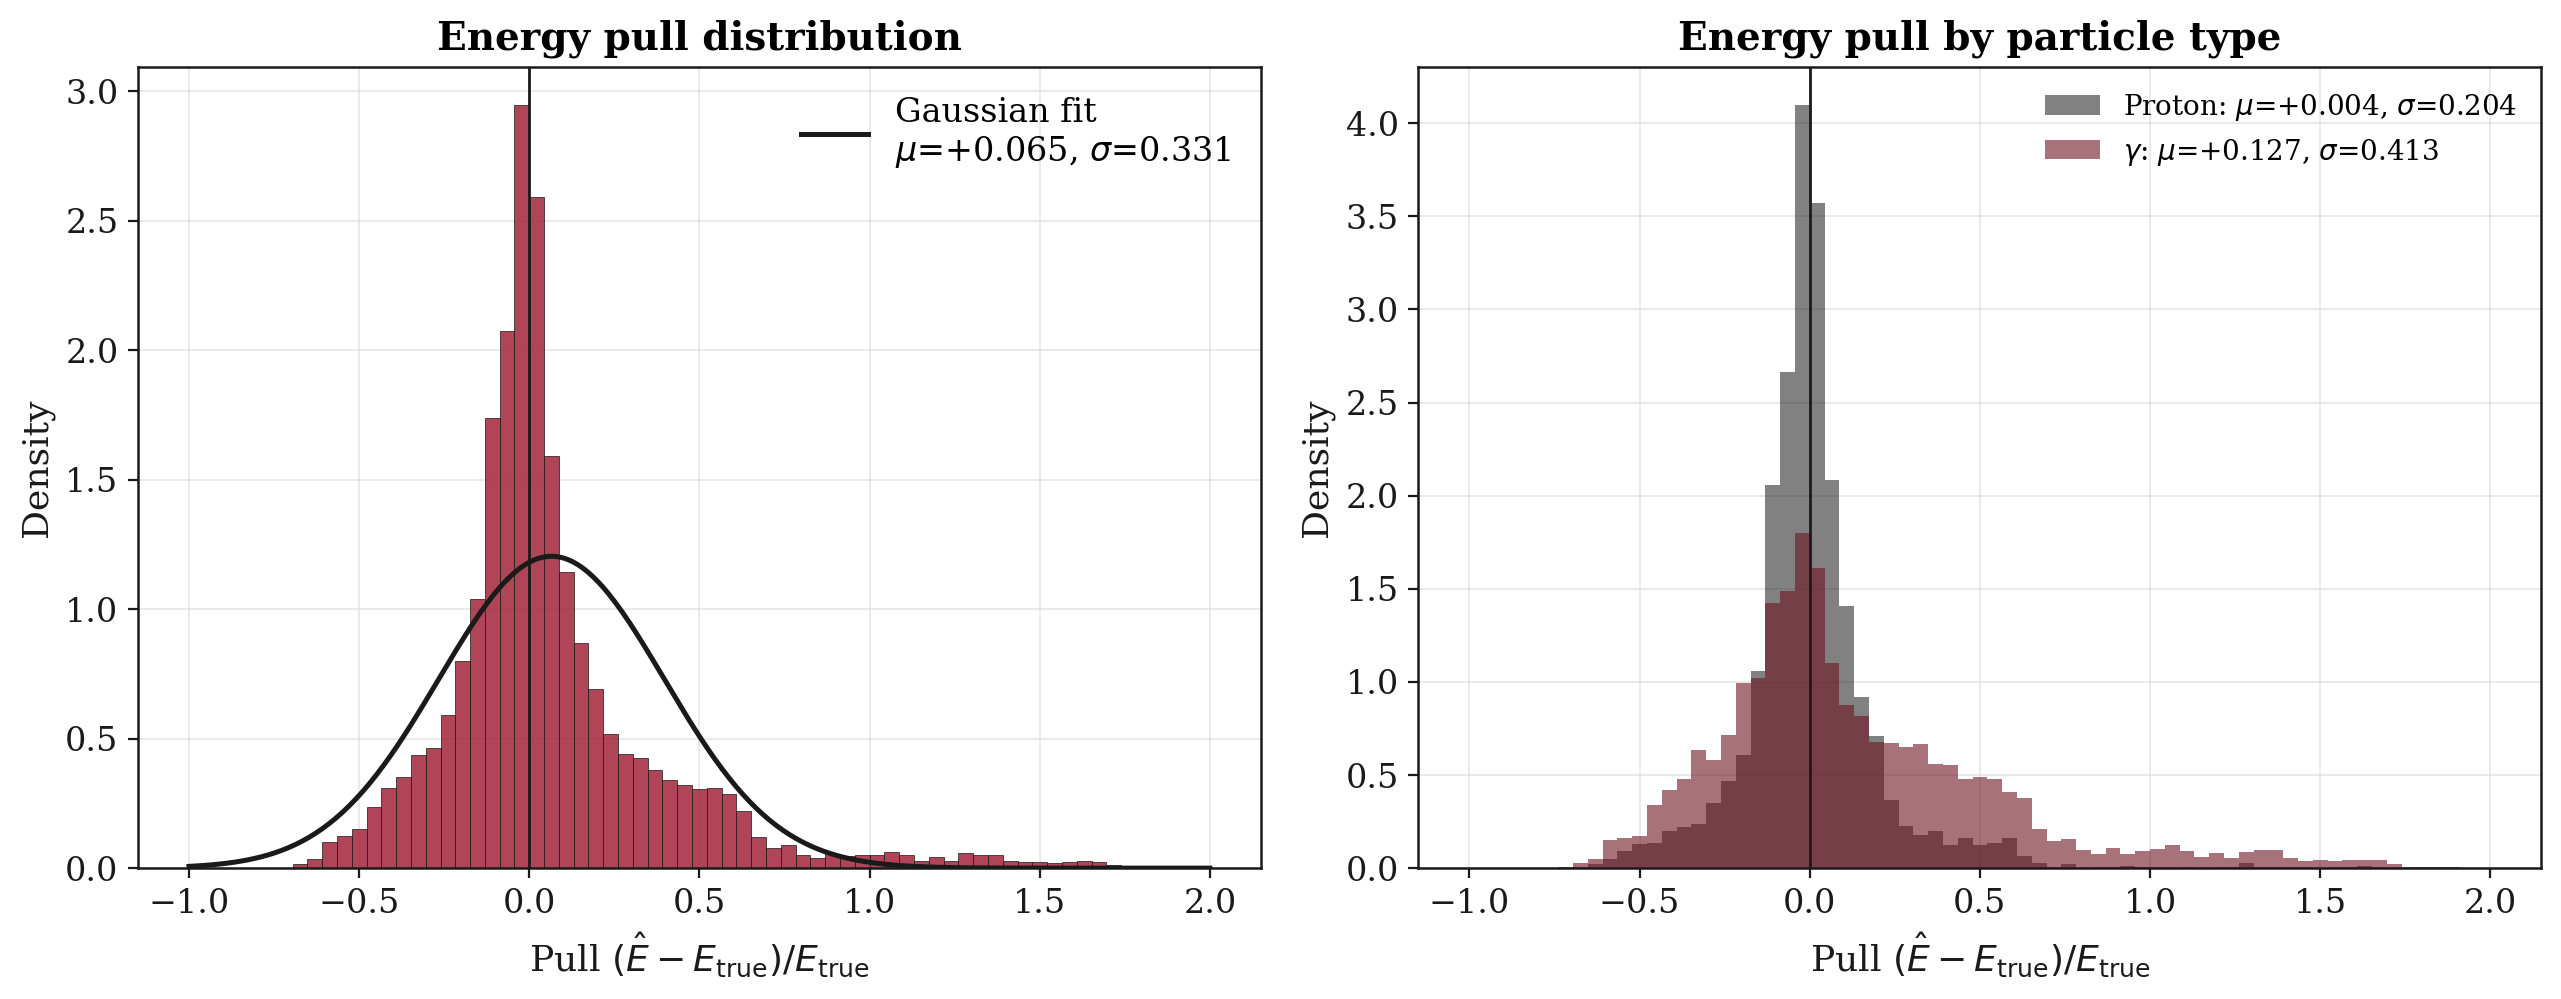
\includegraphics[width=1\linewidth]{figures/energy_analysis.png}
    \caption[Energy pull distribution overall and by particle type.]{Energy estimation analysis. \textbf{Left:} overall pull distribution $(\hat{E} - E_\mathrm{true})/E_\mathrm{true}$ with Gaussian reference curve ($\mu = 0.065$, $\sigma = 0.331$). \textbf{Right:} pull distribution split by particle type; both classes are essentially unbiased but gamma events show roughly twice the width of proton events, consistent with the per-class resolutions in Table~\ref{tab:energy_stratified}.}
    \label{fig:energy_analysis}
\end{figure*}

The energy head produces a continuous estimate, so a rule is required to place each prediction into one of the three energy bins of the dataset. Each event is assigned to the bin whose nominal energy is closest to its prediction, that is, to the value in $\{300, 500, 800\}$~GeV minimizing $|\hat{E} - E_\text{bin}|$. This is equivalent to cutting the continuous axis at the midpoints between consecutive levels, at 400 and 650 GeV. The assignment is used only to build the matrix and plays no part in training or in any of the regression metrics reported above, all of which are computed on the continuous predictions.

Figure~\ref{fig:migration_matrix} shows the resulting energy migration matrix, which reports for each true energy bin the fraction of events reconstructed in each of the three energy bins. The diagonal elements are 75.0\%, 68.2\%, and 67.5\% for 300, 500, and 800 GeV respectively. The largest off-diagonal entry is the 27.8\% migration from 800 GeV to the 500 GeV bin: more than a quarter of high-energy events are systematically reconstructed at a lower energy. This is consistent with the negative bias at 800 GeV identified above and reflects the inherent difficulty of separating 500 and 800 GeV showers in the sub-TeV regime, where the difference in shower size and footprint between adjacent energy bands can be within the natural fluctuation range of individual events.

\begin{figure}[ht!]
    \centering
    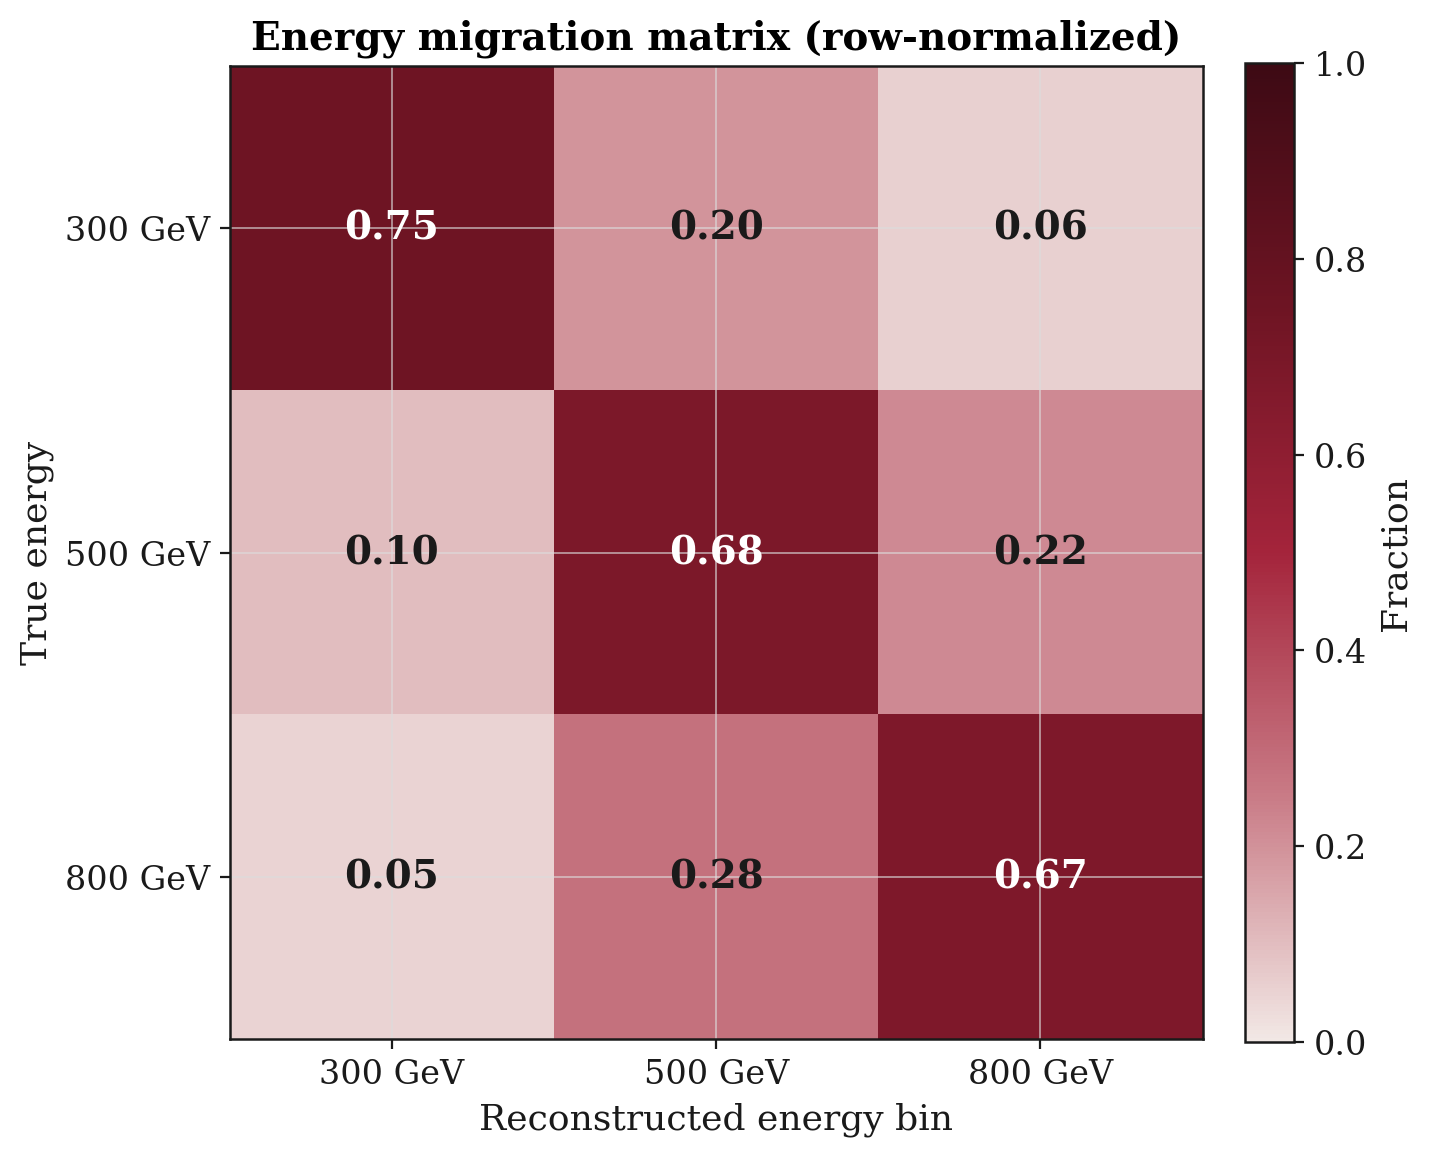
\includegraphics[width=0.62\linewidth]{figures/energy_migration_matrix.png}
    \caption[Energy migration matrix.]{Energy migration matrix. Each row gives the fraction of events at a given true energy that are reconstructed in each of the three energy bins (row-normalized). A dominant diagonal indicates low migration; off-diagonal entries indicate systematic misreconstruction between adjacent energy bins.}
    \label{fig:migration_matrix}
\end{figure}

\subsection{Comparison with the State of the Art}
\label{subsec:sota}

Table~\ref{tab:sota} places the results in the context of prior work on deep learning for EAS reconstruction. Direct comparisons across experiments are complicated by differences in detector technology, altitude, energy range, and the number of simultaneously reconstructed quantities; the table therefore includes the relevant context for each comparison. The model presented in this thesis is the only published work to address three reconstruction tasks simultaneously, at this altitude and energy range, with an integrated explainability framework.

\begin{table}[ht!]
\centering
\caption[Comparison with state-of-the-art EAS reconstruction.]{Comparison with selected published results on deep learning for EAS reconstruction. \textit{Tasks}: number of simultaneously reconstructed quantities (g/h = gamma-hadron, $\theta$ = zenith angle, $E$ = energy). Dashes indicate metrics not reported or not applicable.}
\label{tab:sota}
\renewcommand{\arraystretch}{1.2}
\resizebox{\linewidth}{!}{%
\begin{tabular}{llcclcc}
\toprule
\textbf{Reference} & \textbf{Observatory} & \textbf{Alt.} & \textbf{Energy range} & \textbf{Tasks} & \textbf{g/h AUC} & \textbf{Ang.\ MAE} \\
\midrule
This work & CONDOR & 5,300 m & 300--800 GeV & 3 (g/h, $\theta$, $E$) & \textbf{0.991} & $\mathbf{0.484\degree}$ \\
\shortciteA{navarro2025multi} & CONDOR & 5,300 m & 150--800 GeV & 2 (g/h, $\theta$) & F1=0.89 & $1.14\degree$ \\
\shortciteA{arratia2025condor} & CONDOR & 5,300 m & 100 GeV--1 TeV & $\theta$ & --- & $1$--$2\degree$ \\
\shortciteA{okukawa2024neural} & Tibet AS$\gamma$ & 4,300 m & 10--100 TeV & 1 (g/h) & 0.781--0.901 & --- \\
\shortciteA{erdmann2018deep} & Pierre Auger & 1,400 m & 3--100 EeV & 1 ($\theta$) & --- & $1.2\degree$ \\
\bottomrule
\end{tabular}}
\end{table}

The methods and published results against which this work is compared are described in Section~\ref{sec:related_work}. The angular resolution of $0.484\degree$ represents a factor of 2.4 improvement over the predecessor model~\shortciteA{navarro2025multi} and places the reconstruction well below the 1\degree~threshold typically required for point-source identification in gamma-ray astronomy. The gamma-hadron AUC of 0.991 is achieved at a substantially lower energy range and with a more complex multi-task constraint than the comparable scintillator-array results of~\shortciteA{okukawa2024neural}, who report AUC values of 0.781--0.901 at 10--100 TeV on a single-task network. The most directly comparable gamma-hadron study in our energy window is that of~\shortciteA{conceiccao2025discriminating}, who apply a pretrained vision transformer to the shower footprint of a water-Cherenkov array at 5{,}200~m over the 200~GeV--1~TeV range, reporting a proton rejection of approximately 97\% at a gamma efficiency of 80\%. 

A direct AUC comparison with their work is not possible because they quote performance at fixed efficiency working points rather than a threshold-integrated metric, and their detector technology (water Cherenkov) differs from the CONDOR scintillator array; nonetheless, their results corroborate that sub-TeV footprint morphology carries strong discriminating power. Energy estimation, by contrast, is not directly comparable across experiments, as the energy ranges and figures of merit differ substantially: \shortciteA{meng2025machine}, for instance, reconstruct primary energy for Tibet AS$\gamma$ but over the 1~TeV--10~PeV range, where the resolution behaves intrinsically differently. The migration matrix in Figure~\ref{fig:migration_matrix} therefore provides the most informative characterization of energy reconstruction quality for this work.

% ============================================================
\section{Explainability Analysis}
\label{sec:explainability}
% ============================================================

Two complementary feature importance methods --- a feature ablation study and permutation feature importance --- are applied to validate that the learned representations are physically consistent. Because both quantify the same notion (the degradation in task performance when a single input feature is disabled) and yield mutually consistent rankings, they are presented together. They are followed by an analysis of the attention patterns extracted from the RAW Transformer streams, which provide hit-level interpretability directly in the space of detector observables.

\subsection{Feature Importance}
\label{subsec:feature_importance}

The term \emph{ablation} is borrowed from experimental neuroscience, where lesion studies selectively remove or disable a region of the brain and infer the function of that region from the behavioural deficit that follows; the same methodology was later adopted to probe the internal representations of artificial neural networks~\shortciteA{meyes2019ablation}. The \textbf{feature ablation study} applies this logic at the level of the input: it measures the importance of each input feature by replacing it with its median value across the training set --- computed over non-padded positions only --- and evaluating the resulting degradation in test-set performance, attributing the loss to the information that the disabled feature carried.

\textbf{Permutation feature importance} (PFI)~\shortciteA{altmann2010permutation} instead randomly permutes a single feature across all test-set events, breaking its correlation with the target while preserving its marginal distribution. The two are complementary: ablation collapses a feature to a single typical value and is therefore sensitive to the loss of its typical variation, whereas PFI preserves the full distribution and is more sensitive to the information carried by a feature's extreme values. Both methods are applied independently to each of the six sequential features --- \texttt{detector\_id}, \texttt{particle\_count}, \texttt{t\_bin}, \texttt{total\_energy}, \texttt{x\_center}, and \texttt{y\_center} --- for each of the three tasks. Figures~\ref{fig:ablation} and~\ref{fig:pfi} report the relative degradation, expressed as a percentage of the baseline metric, for ablation and PFI respectively.

\textbf{Zenith angle.} Both methods agree that \texttt{t\_bin} is by far the most important feature for angular reconstruction. Ablation increases the MAE from its baseline of $0.484\degree$ to $12.9\degree$ (a relative degradation of approximately 2{,}568\%), and PFI yields a comparable $\Delta\text{MAE} = 12.76\degree$. This is physically expected: the arrival time of each detector hit encodes the position of the shower wavefront, and the gradient of arrival times across the array is the primary observable from which the zenith angle is geometrically determined. The next most important features are the spatial coordinates \texttt{x\_center} (ablation $+9.1\degree$, 1{,}889\%; PFI $+5.1\degree$) and \texttt{detector\_id} (ablation $+7.0\degree$, 1{,}456\%; PFI $+3.3\degree$), consistent with the geometric nature of the task.

\textbf{Gamma-hadron discrimination.} For classification both methods place energy deposition and spatial position at the top, with a minor reordering between them. Ablation ranks \texttt{total\_energy} first (accuracy drop of 0.224, a relative degradation of 23.1\%), followed by \texttt{x\_center} (0.136, 14.0\%) and \texttt{t\_bin} (0.118, 12.2\%); PFI ranks \texttt{x\_center} first (0.338, 34.8\%), then \texttt{total\_energy} (0.257, 26.5\%) and \texttt{t\_bin} (0.220, 22.7\%). The prominence of \texttt{total\_energy} reflects the role of the per-hit deposited energy as a tracer of local particle density: electromagnetic showers concentrate this density in a compact core while hadronic showers spread it more widely and irregularly, so the spatial pattern of per-hit energy deposits carries the morphological signature that distinguishes the two classes. The reordering between the two methods reflects the redundancy among the positional features (\texttt{detector\_id}, \texttt{x\_center}, and \texttt{y\_center} all encode hit location): permuting one while leaving the others intact allows partial compensation, distributing the measured importance across the correlated features. Both methods point to a discrimination strategy based on the energy-weighted lateral distribution rather than on single-detector particle identification.

\textbf{Energy estimation.} Spatial position dominates energy reconstruction. Ablation ranks \texttt{x\_center} first ($+106.4$ GeV, 102.6\%), followed by \texttt{detector\_id} ($+83.4$ GeV) and \texttt{t\_bin} ($+72.7$ GeV); PFI ranks \texttt{t\_bin} first ($\Delta\text{MAE} = 173.3$ GeV), followed by \texttt{x\_center} ($143.9$ GeV) and \texttt{detector\_id} ($103.6$ GeV). The spatial position of active hits encodes the shower's lateral extent, which is the strongest predictor of primary energy in ground-based EAS experiments; the prominence of \texttt{t\_bin} under PFI reflects the additional information carried by the full temporal spread of the shower development. Across all three tasks and both methods, \texttt{particle\_count} is the least informative feature (accuracy drop $<0.01$, MAE increase $<1$ GeV), indicating that the number of particles at a given detector adds little beyond what the deposited energy already captures.

\begin{figure*}[ht!]
    \centering
    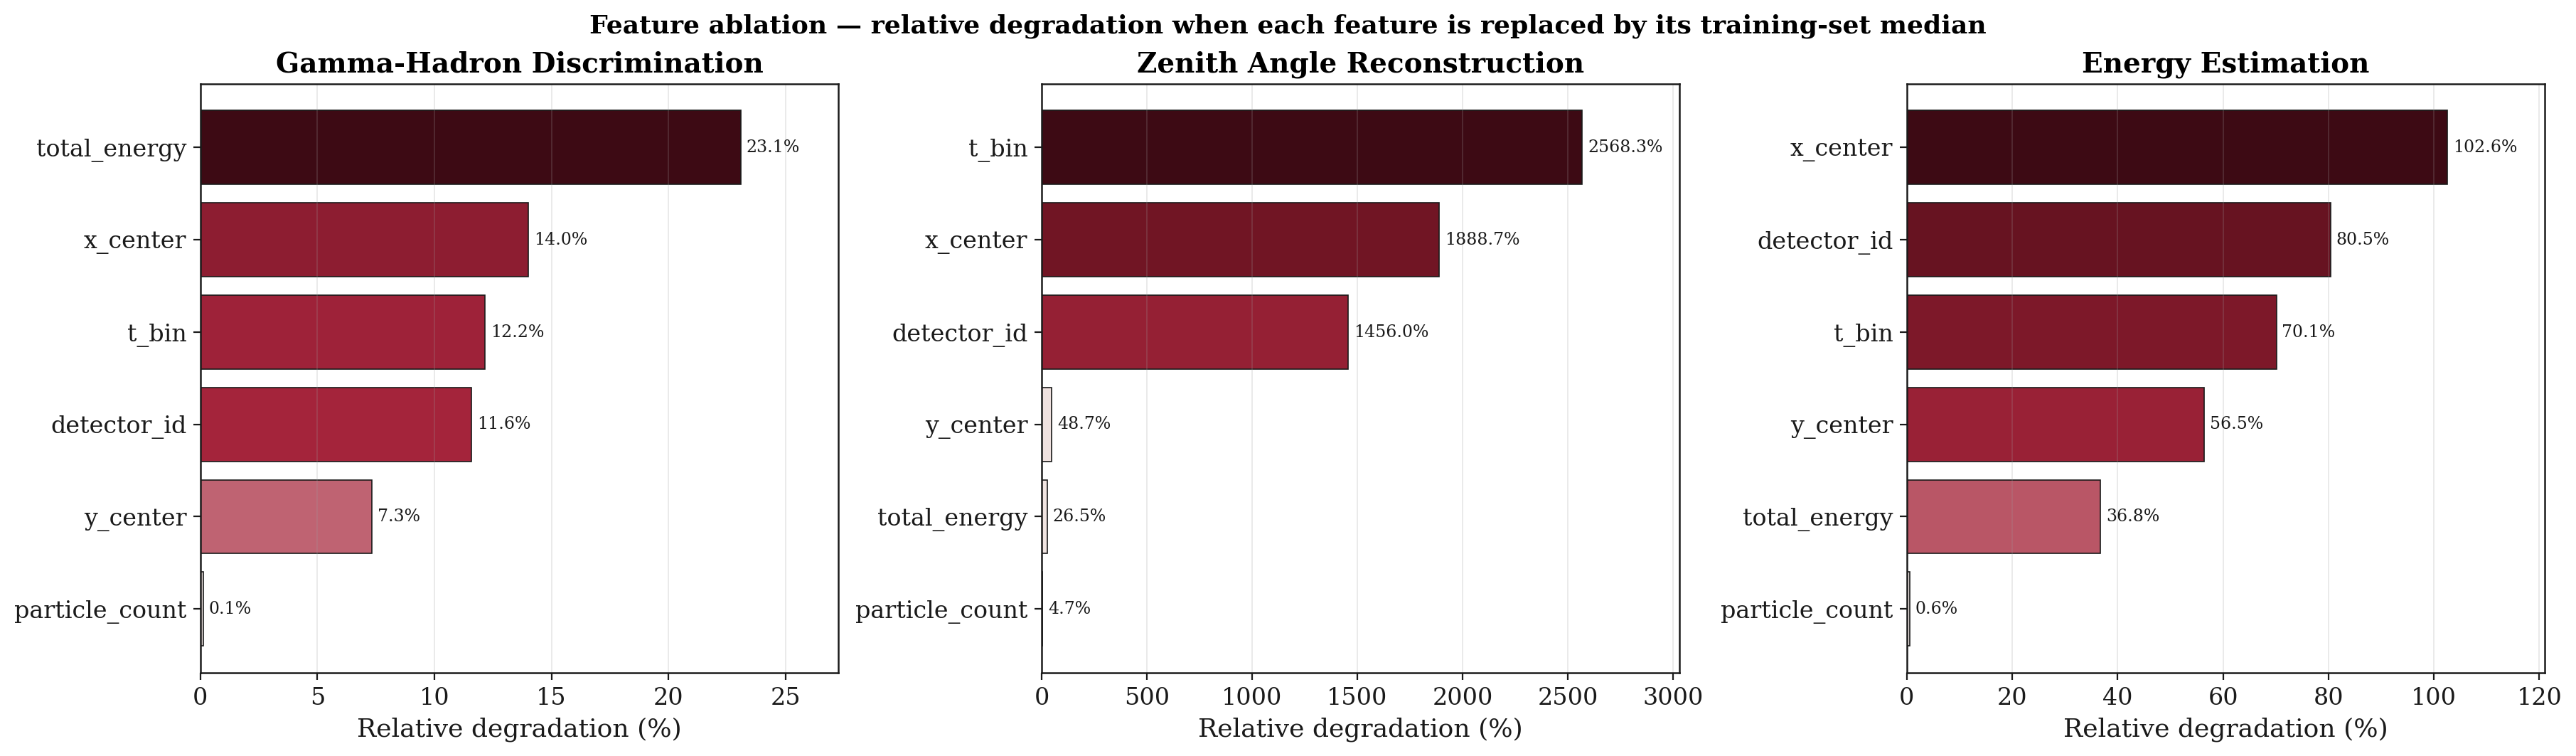
\includegraphics[width=1\linewidth]{figures/feature_ablation.png}
    \caption[Feature ablation study results.]{Feature ablation study: relative degradation, expressed as a percentage of the baseline metric, when each feature is replaced by its training-set median. Each panel corresponds to one reconstruction task; bars are ordered by magnitude and shaded by it.}
    \label{fig:ablation}
\end{figure*}

\begin{figure*}[ht!]
    \centering
    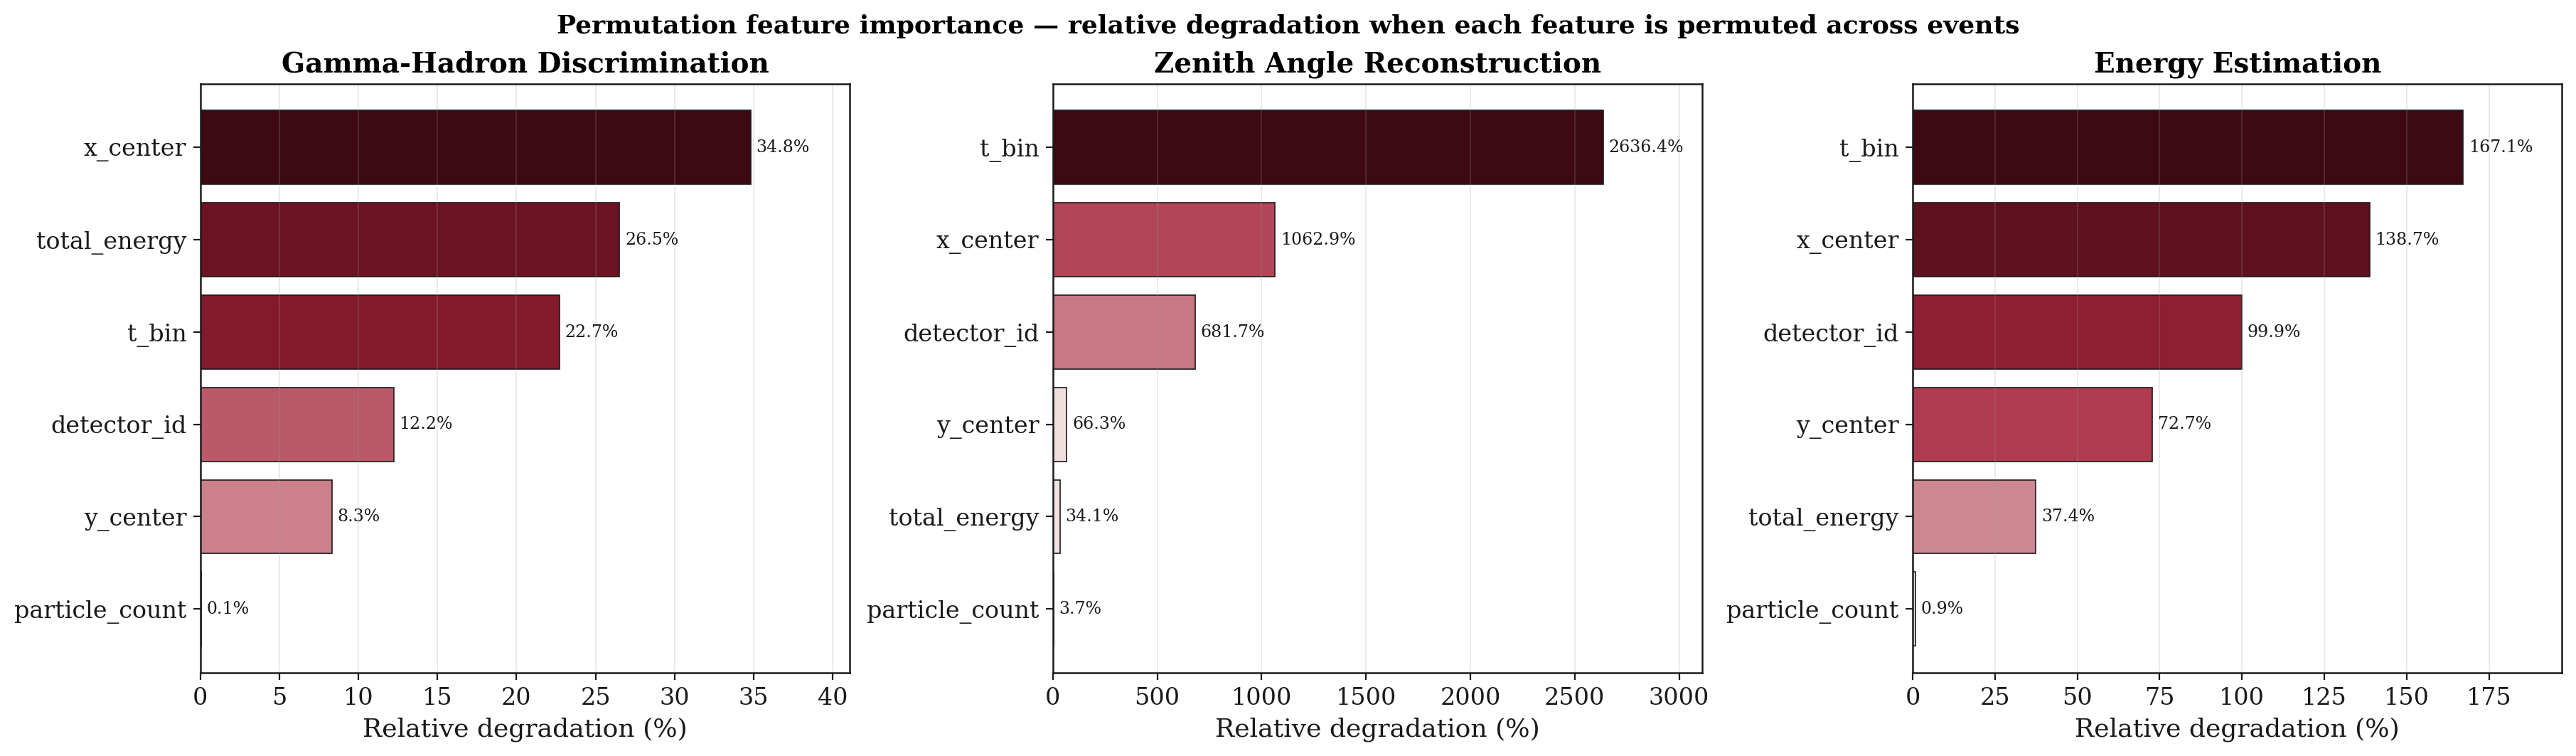
\includegraphics[width=1\linewidth]{figures/pfi_results.png}
    \caption[Permutation feature importance results.]{Permutation feature importance (PFI): relative degradation, expressed as a percentage of the baseline metric, when each feature is permuted across all test-set events. Each panel corresponds to one reconstruction task.}
    \label{fig:pfi}
\end{figure*}

\subsection{Attention Analysis}
\label{subsec:attention}

The RAW Transformer streams operate directly on the masked hit sequence, so their attention weights can be examined at the level of individual detector hits. For an event with $L$ valid hits, $\alpha_{ij}$ denotes the weight that query position $i$ assigns to key position $j$. The weights are produced by a softmax over the valid keys, so that $\sum_{j=1}^{L} \alpha_{ij} = 1$. Two views are reported. The first is the mean attention matrix, averaged over events. The second is the mean attention received by each position,
\begin{equation}
    \bar{\alpha}_{\cdot j} = \frac{1}{L}\sum_{i=1}^{L} \alpha_{ij},
    \label{eq:mean_key_attention}
\end{equation}
which identifies the positions that act as information sources for a stream. Because each row sums to unity, a position of average importance receives a weight of $1/L$; for the mean sequence length of 76.9 valid hits, this reference level is $1.3 \times 10^{-2}$. Hits are ordered chronologically, so low position indices correspond to early-arriving hits, near the leading edge of the shower front. The analysis uses a stratified subsample of 200 test events and the first 120 sequence positions.

\begin{figure*}[ht!]
    \centering
    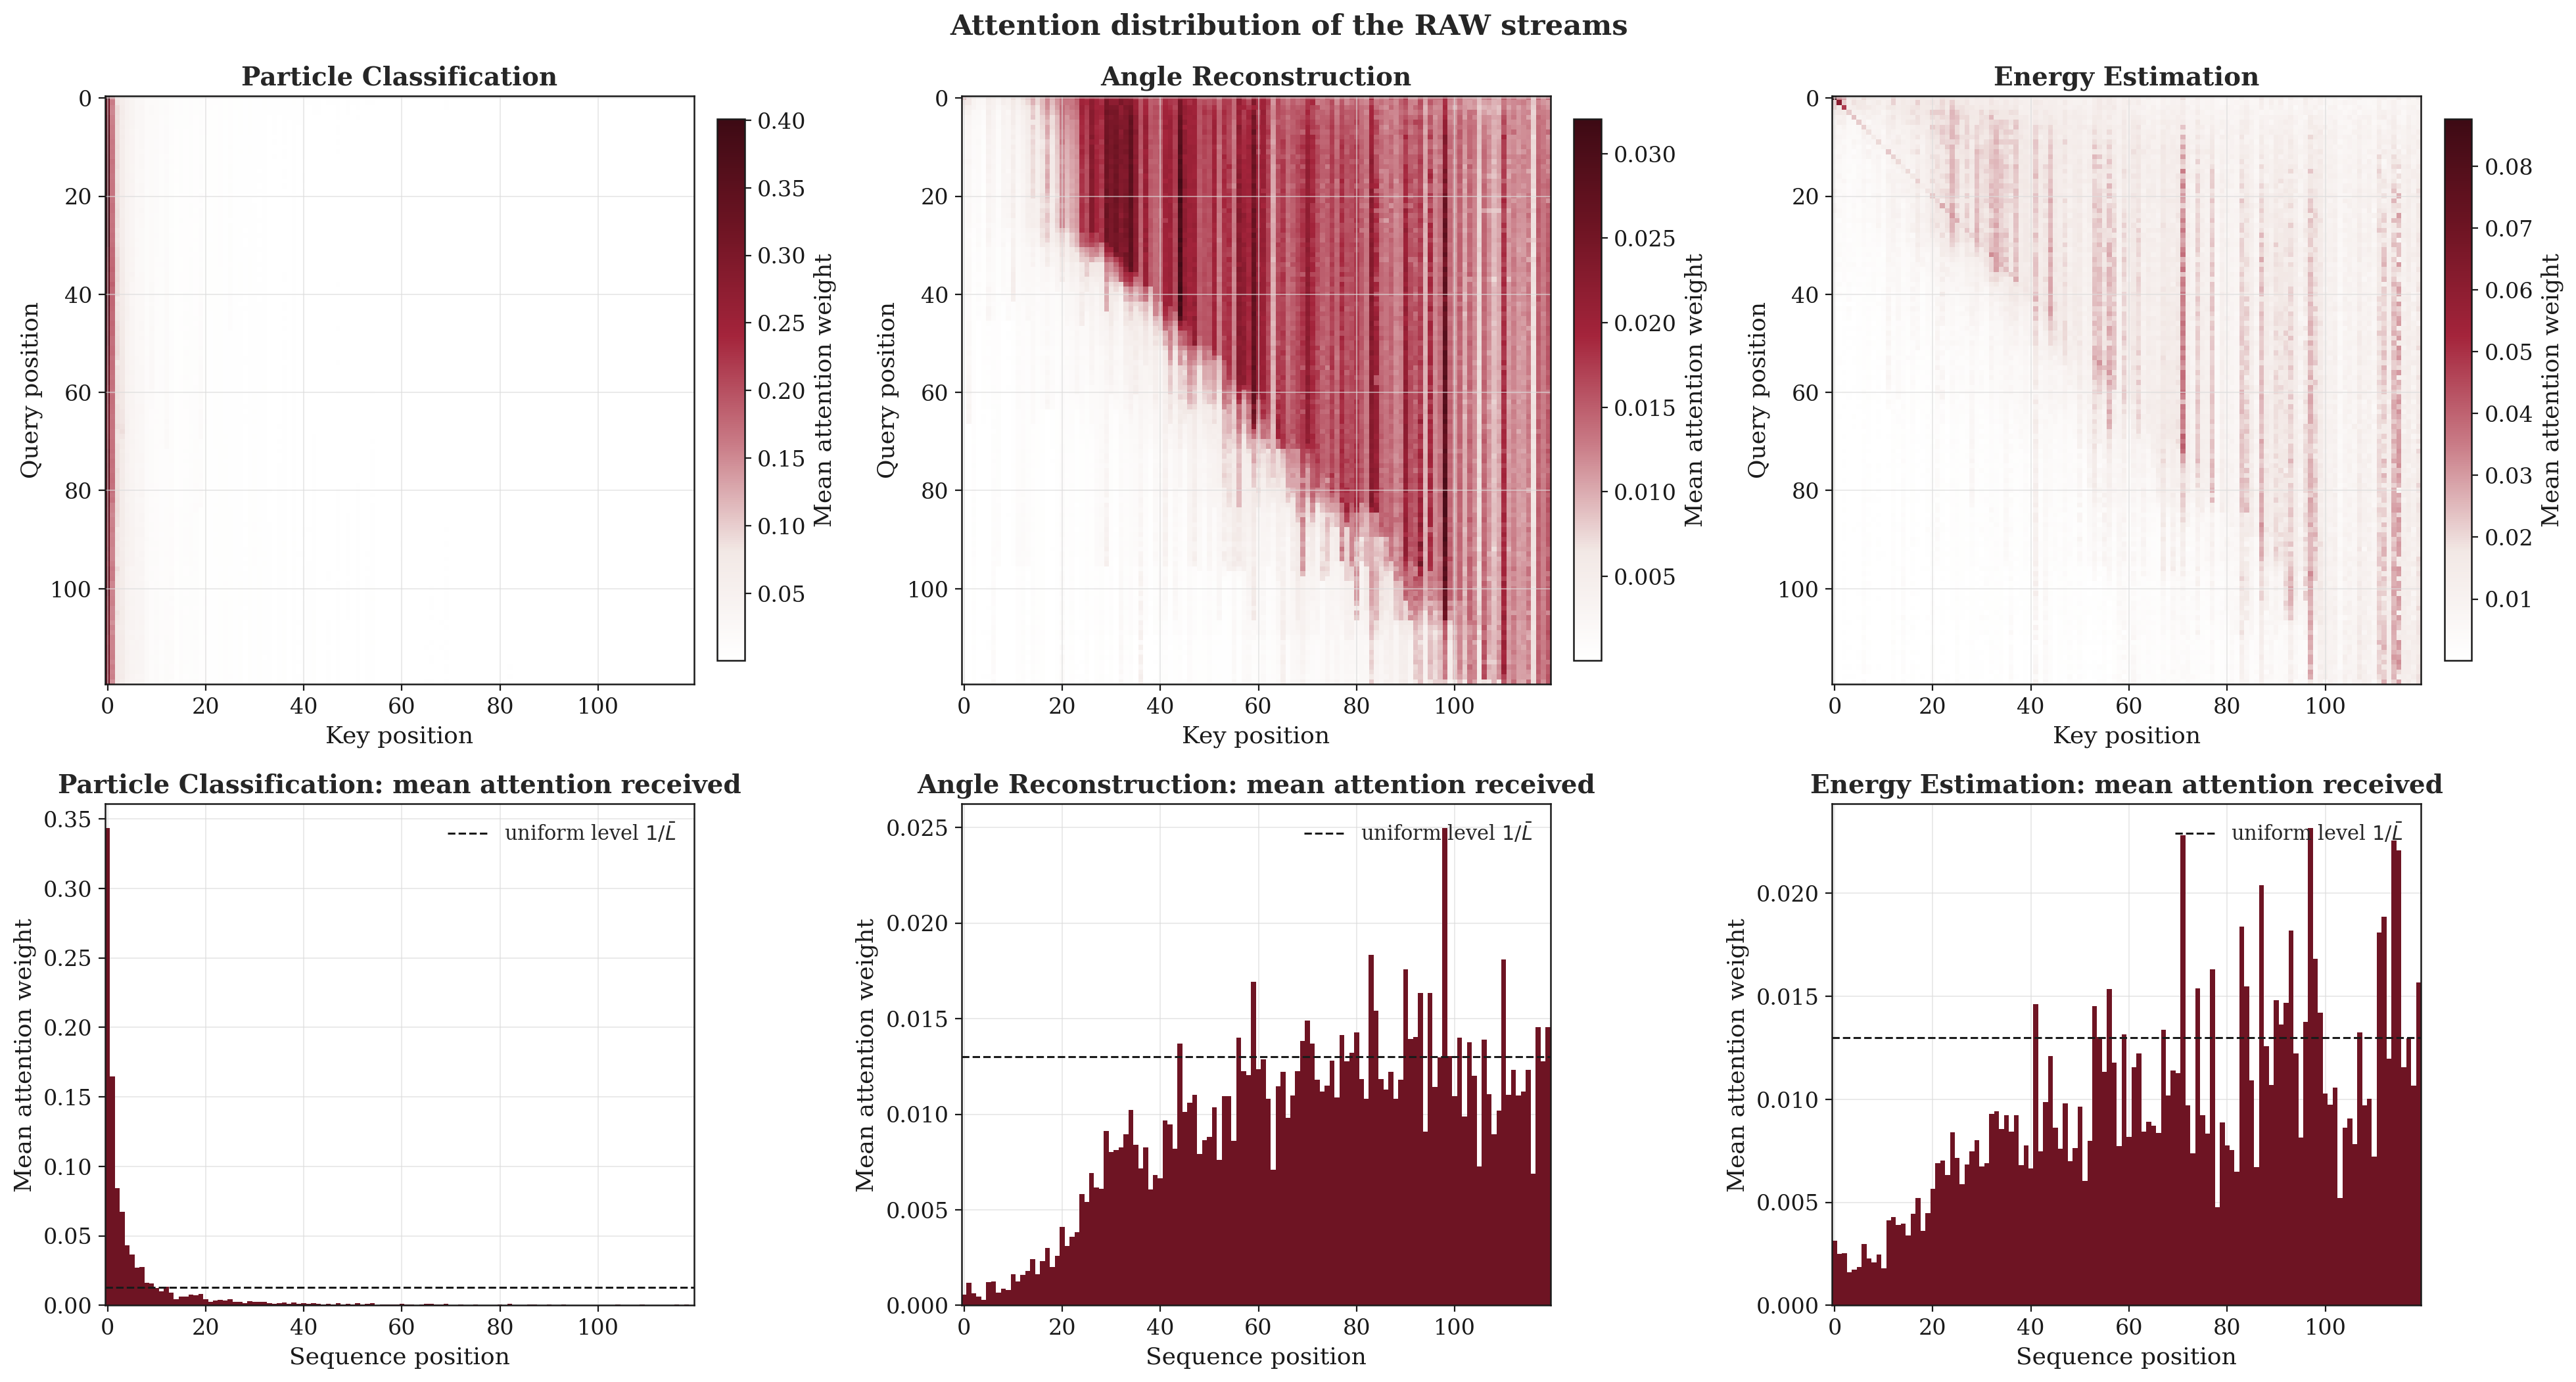
\includegraphics[width=1\linewidth]{figures/attention_patterns_raw.png}
    \caption[Attention distribution of the RAW streams.]{Attention distribution of the three RAW streams. \textbf{Top:} mean attention matrix, averaged over 200 test events; rows are query positions and columns are key positions. \textbf{Bottom:} mean attention received per position, Equation~\eqref{eq:mean_key_attention}; the dashed line marks the uniform reference level $1/\bar{L} = 1.3 \times 10^{-2}$. Cells averaged over fewer than ten events are left blank.}
    \label{fig:attention_patterns}
\end{figure*}

Figure~\ref{fig:attention_patterns} shows both views for the three streams, and the distributions differ markedly between tasks. The classification stream concentrates its weight on the leading edge of the sequence: the first position receives a mean weight of $0.34$, twenty-six times the uniform level, only the first thirteen positions exceed that level, and $82\%$ of the profile lies within the first ten positions. Equivalently, $93\%$ of the matrix weight is assigned to keys that precede the query.

The angle stream shows the opposite ordering. Its profile grows with position, exceeds the uniform level only beyond position 44, and peaks at $2.5 \times 10^{-2}$ near position 98, with $0.7\%$ of the profile in the first ten positions. Correspondingly, $80\%$ of the matrix weight is assigned to keys that follow the query, producing the triangular structure visible in the mean matrix. The energy stream is intermediate: $75\%$ of its weight also falls on later keys, but instead of the smooth ramp of the angle stream the matrix shows isolated bands at specific positions, and a weak diagonal component in which positions attend to their own neighbourhood.

These distributions are consistent with the feature importance results of Section~\ref{subsec:feature_importance}. Zenith angle reconstruction is dominated by \texttt{t\_bin} under both ablation and permutation, and the angle stream accordingly draws its weight from the late part of the sequence, where the arrival-time gradient across the array is defined. Gamma-hadron discrimination depends most strongly on the deposited energy and on the spatial coordinates, quantities that the leading hits already characterize, and the classification stream concentrates on precisely that region. Energy estimation shows the least specialized pattern of the three, which matches its position as the task with the lowest reconstruction quality.

\textbf{Interpretive scope of the attention maps.} Attention weights describe how a stream distributes its reads over the input sequence. They are not an attribution of the prediction to those inputs, and a large weight is not by itself evidence that the corresponding hit was used causally~\shortcite{jain2019attention}. The distributions above are therefore reported as a description of the model's internal weighting, and the feature-level conclusions of this chapter rest on the ablation and permutation analyses of Section~\ref{subsec:feature_importance}, which intervene on the input, measure the resulting change in reconstruction performance, and agree with each other. The limitations of attention-based explainability are discussed further in Section~\ref{sec:limitations}.

% ============================================================
\section{Detector Robustness and Array Optimization}
\label{sec:robustness}
% ============================================================

Because CONDOR is still a proposed observatory, the trained model can be used to answer two practically important questions: how much reconstruction performance degrades as detectors fail, and whether the current array layout uses its detectors efficiently. This section addresses these questions through a \textit{detector switch-off} procedure applied at inference time, without any retraining. 

Concretely, for a chosen set of detectors to be switched off, every hit recorded by those detectors is deleted from each test event, the event's sequential representation is rebuilt from the surviving hits, and the five event-level global features (total particle count, total and central deposited energy, active-detector count, and duration) are recomputed from that reduced hit set. The already-trained model is then evaluated on these modified events, and the resulting change in each task metric relative to the intact-array baseline quantifies how much the model relied on the removed detectors. Events that lose all of their hits are excluded from the corresponding evaluation.

This procedure measures the \textit{dependence} of the trained model on specific detectors, which serves as a proxy for their information content. It is important to note that a model retrained from scratch on a reduced detector configuration could in principle learn compensatory representations that partially recover the lost information; the degradation reported here therefore represents an upper bound on the actual performance loss under detector failure. All experiments in this section are performed on the same stratified subsample of 3{,}000 test events, on which the intact-array baseline is a classification accuracy of $96.7\%$ with an F1-score of $0.967$ and an AUC of $0.990$, an angular MAE of $0.49\degree$, and an energy MAE of $107$~GeV.

\subsection{Single-Detector Importance}
\label{subsec:single_detector}


Figure~\ref{fig:dropout_single} shows the degradation in each task metric when each of the 120 detectors is individually switched off. The spatial maps reveal a clear core-periphery gradient: detectors near the geometric center of the array are individually more critical than peripheral detectors for all three tasks. This is physically expected, since the shower core passes through or near the center of the array for most events in the dataset, and central detectors sample the highest-density region of the particle distribution, which is the most discriminative for both particle type and energy.

\begin{figure*}[ht!]
    \centering
    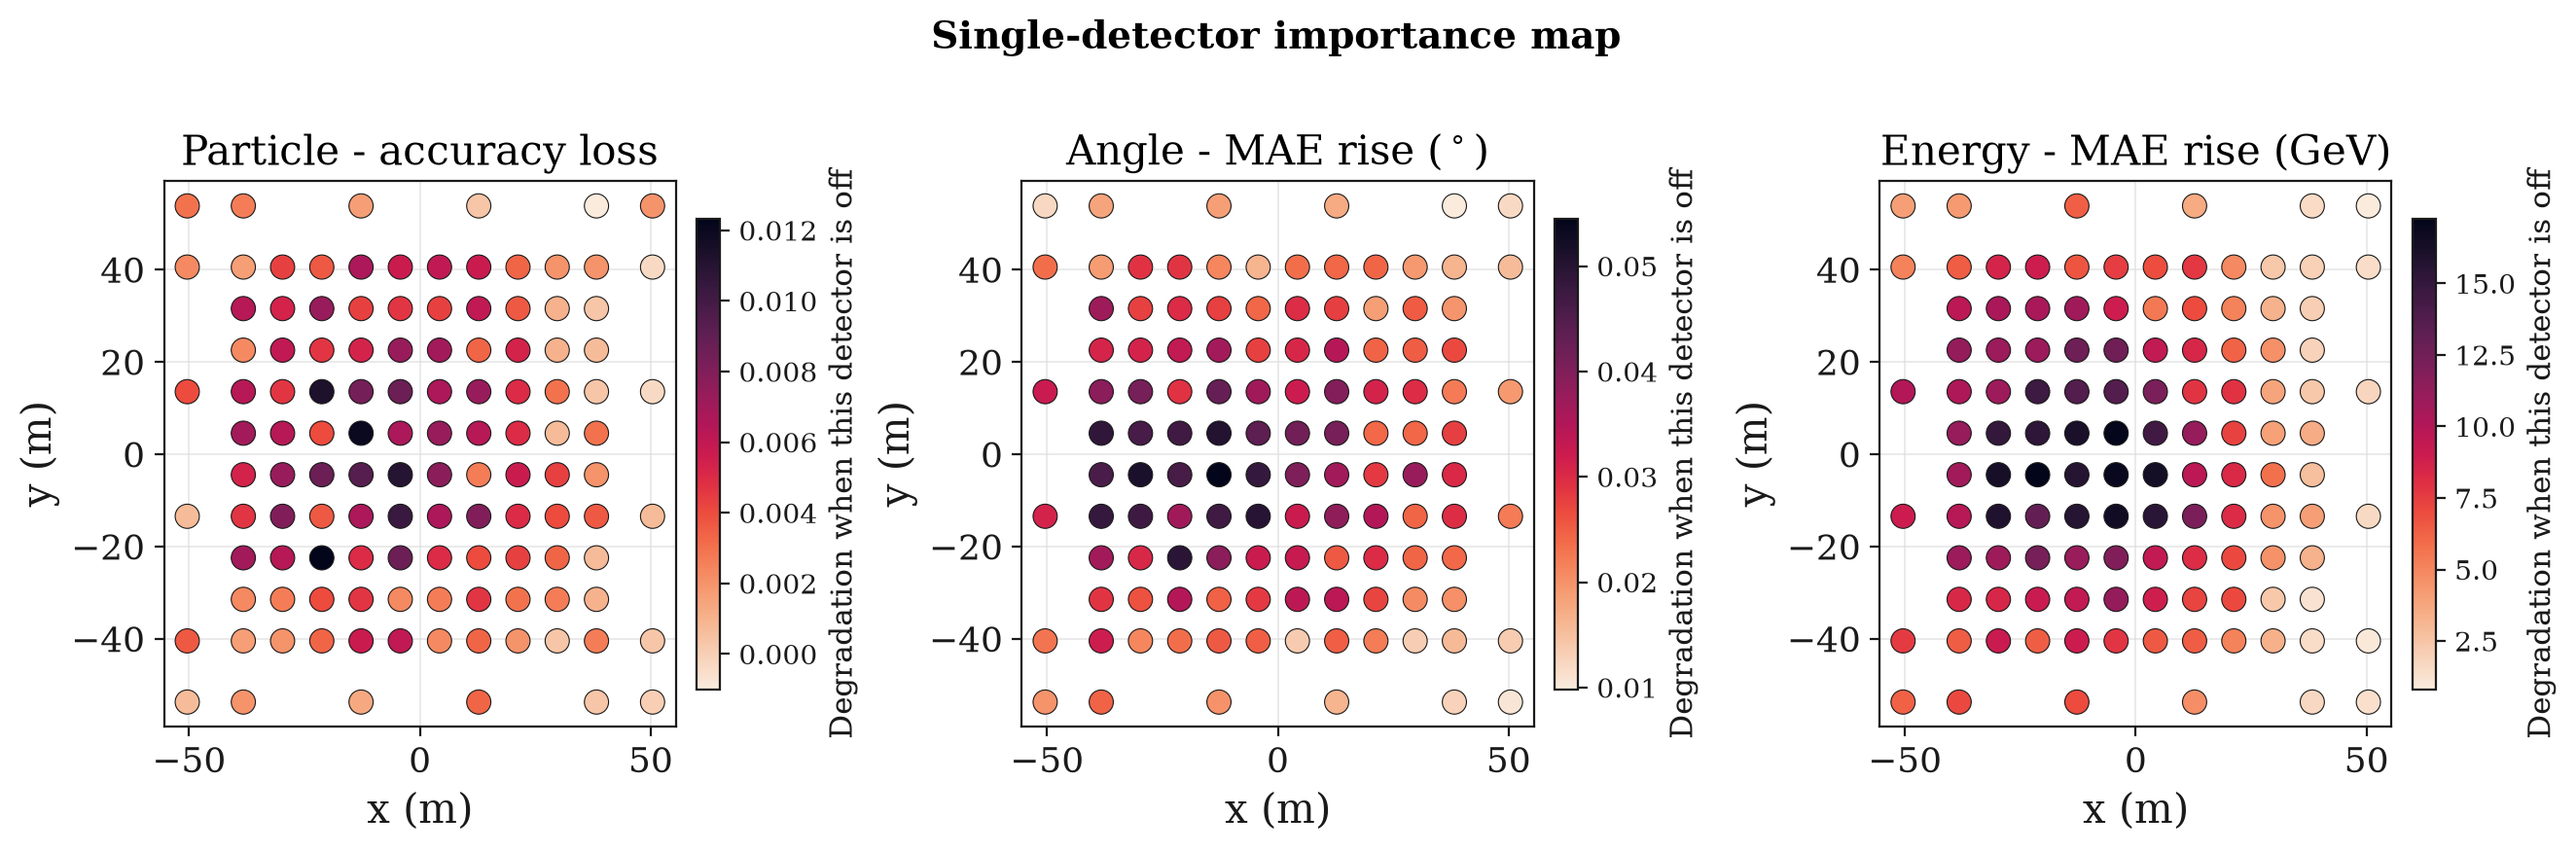
\includegraphics[width=1\linewidth]{figures/dropout_single.png}
    \caption[Single-detector importance map.]{Degradation in each task metric when each detector is individually switched off. Brighter colors indicate detectors whose loss causes the largest performance drop. The core-periphery gradient is consistent across all three tasks.}
    \label{fig:dropout_single}
\end{figure*}

\subsection{Regional Dropout}
\label{subsec:regional}

Two families of geometrically coherent detector groups are switched off simultaneously, defined in Figure~\ref{fig:dropout_regions_map}. The first follows how the array is built: the 100 modules of the central grid are split into the 36 closest to the array centre (\emph{central core}) and the 64 that surround them (\emph{outer grid}), and the 20 peripheral modules, which form a structurally separate sub-array, are kept as their own group. The second family consists of the four halves of the array, $x<0$, $x>0$, $y<0$ and $y>0$, each containing exactly 60 modules and together covering it completely.

\begin{figure}[ht!]
    \centering
    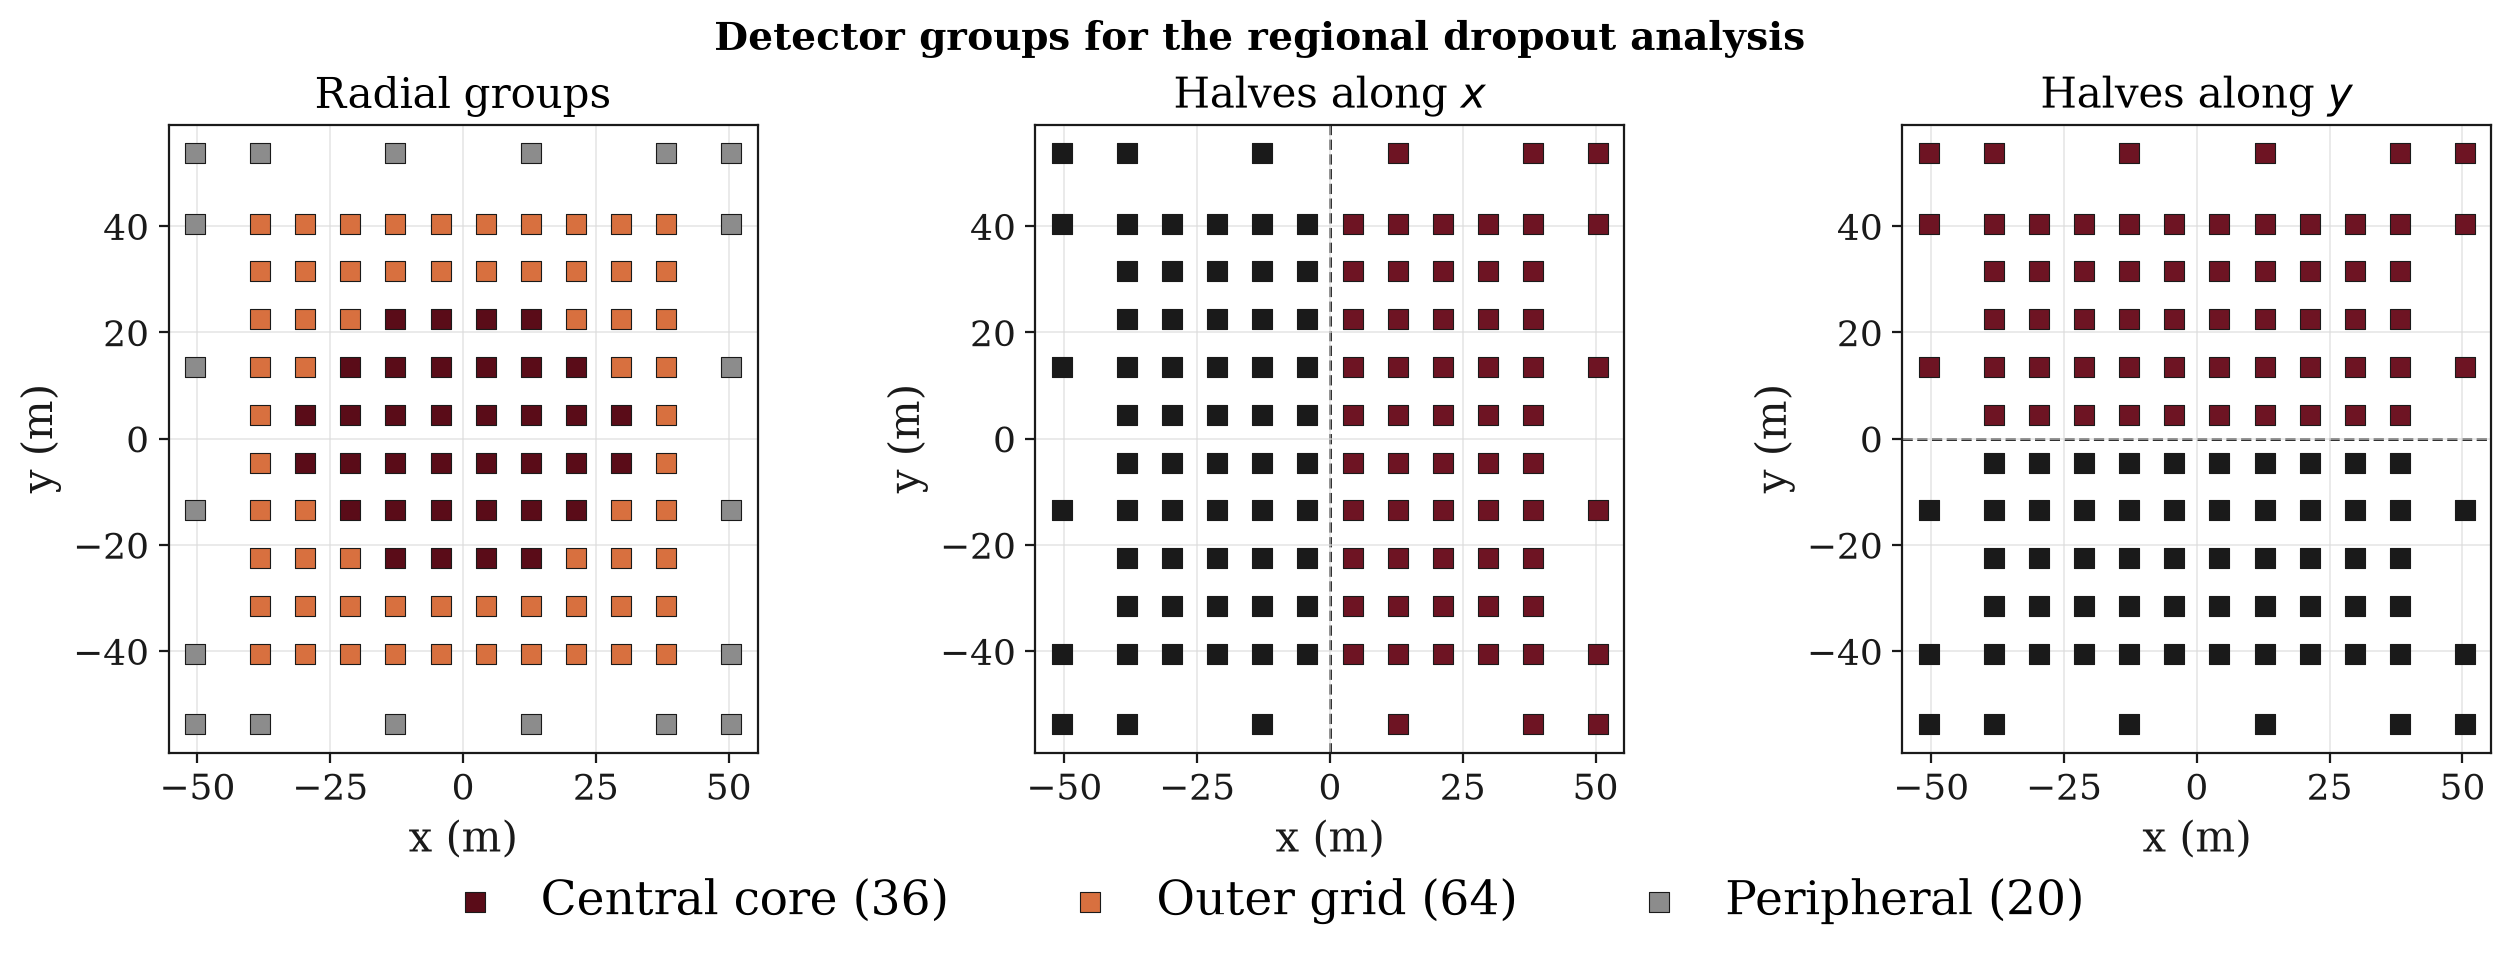
\includegraphics[width=1\linewidth]{figures/dropout_regions_map.png}
    \caption[Detector-group definitions for the regional dropout analysis.]{Spatial definition of the detector groups switched off in the regional dropout analysis. \textbf{Left:} the three radial groups --- the 36 modules closest to the array centre, the remaining 64 modules of the central grid, and the 20 peripheral modules. \textbf{Centre and right:} the four halves, split along $x$ and along $y$, of 60 modules each. The $y$ pair acts as a control for the $x$ pair: the simulated showers all arrive at azimuth $\phi = 0\degree$, which singles out the $x$ direction and should leave the $y$ halves equivalent. Marker positions correspond to the physical module locations on the array.}
    \label{fig:dropout_regions_map}
\end{figure}

Figure~\ref{fig:dropout_regional} quantifies the impact of removing each of these groups. The groups differ in size, and a larger group degrades performance more simply because it removes more detectors. Every quantity is therefore reported both as the degradation caused by removing the whole block, which corresponds to an operational failure of that block, and normalized by the number of detectors removed, which measures the contribution of an individual module. The two rankings do not coincide.

\begin{figure}[ht!]
    \centering
    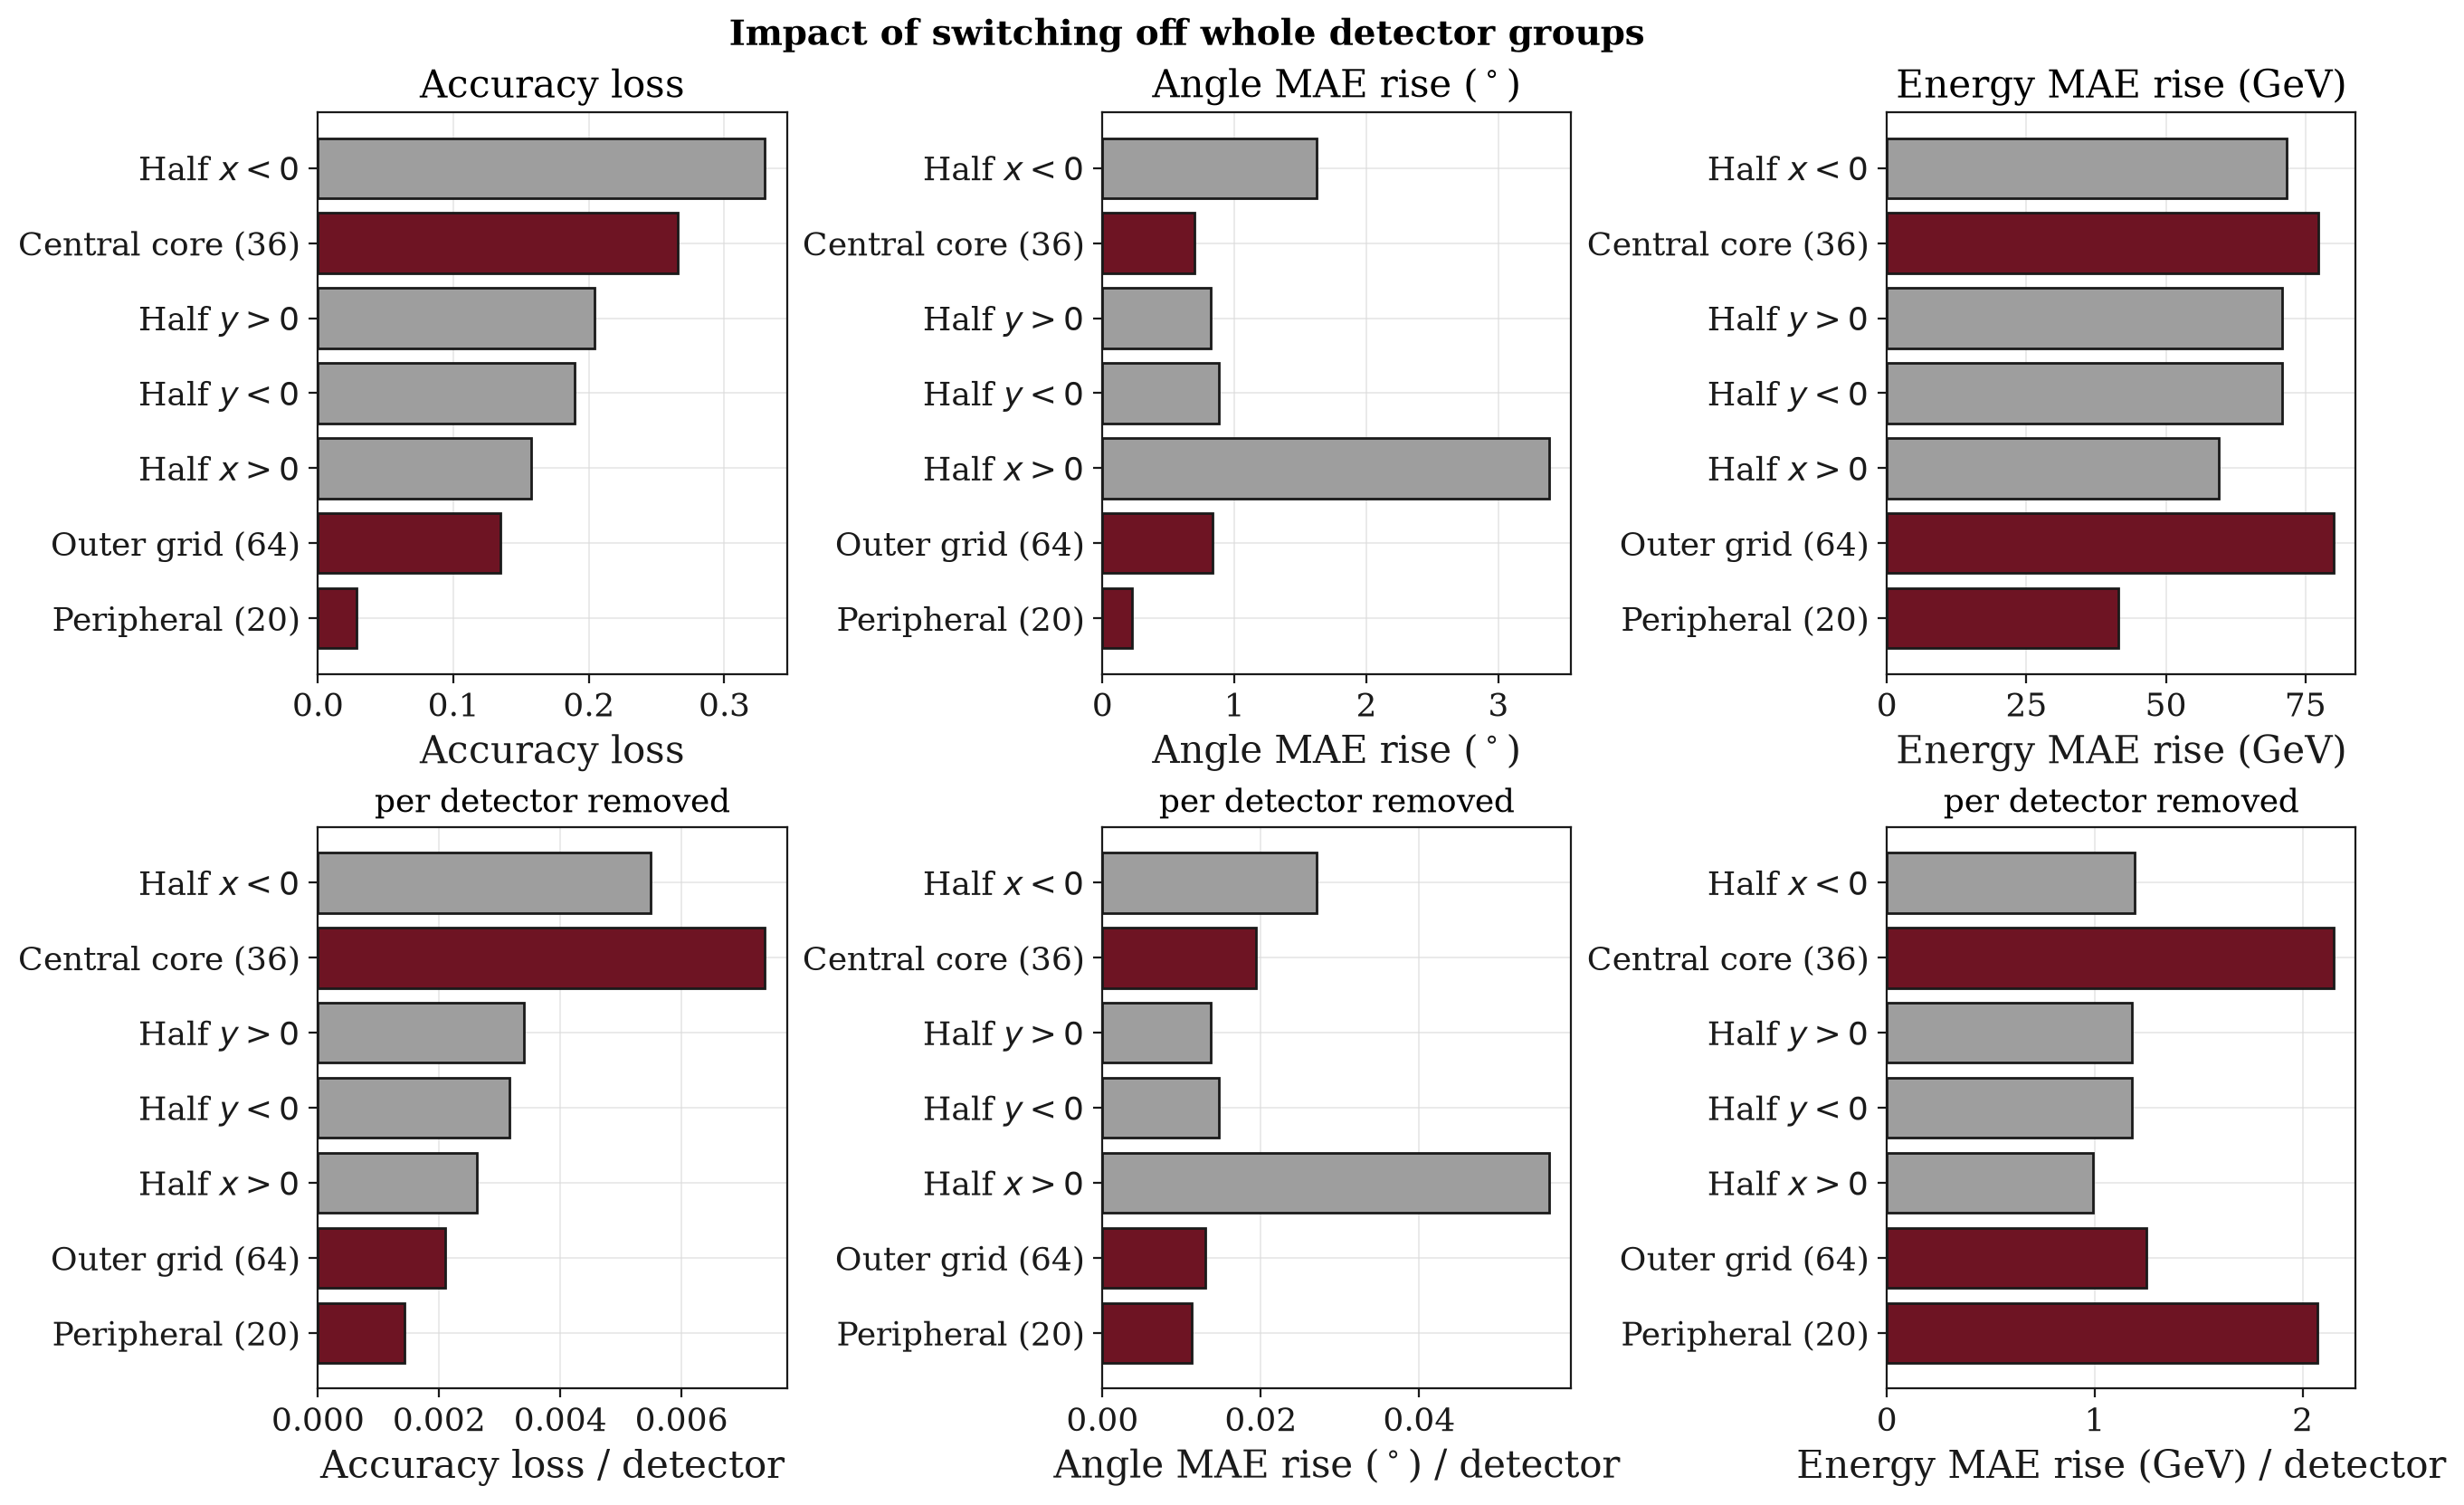
\includegraphics[width=1\linewidth]{figures/dropout_regional.png}
    \caption[Impact of switching off whole detector groups.]{Performance degradation when entire detector groups are removed, sorted by increasing impact on particle accuracy. \textbf{Top:} degradation caused by removing the whole block. \textbf{Bottom:} the same degradation per detector removed, which controls for the different group sizes. Dark red marks the three radial groups, grey the four halves.}
    \label{fig:dropout_regional}
\end{figure}

The three tasks do not depend on the same region of the array. For gamma-hadron classification the ordering follows the core-to-periphery one: removing the central core costs $0.265$ in accuracy, a relative degradation of $27.4\%$, against $13.9\%$ for the outer grid and $3.0\%$ for the 20 peripheral modules. The core achieves this while removing half as many detectors as the outer grid, so per detector it is three and a half times more damaging ($7.4 \times 10^{-3}$ against $2.1 \times 10^{-3}$ accuracy per module). Classification depends on the high particle density near the shower core, which only the central modules sample.

For angular reconstruction the ordering differs. Removing the outer grid raises the angular MAE by $0.83\degree$ ($171\%$), more than the $0.70\degree$ ($144\%$) caused by removing the central core; this is the only task for which the core is not the most damaging block. Per detector the core remains the more critical of the two ($1.9 \times 10^{-2}$ against $1.3 \times 10^{-2}$ degrees per module), so the outer grid leads as a block because it holds 64 modules against 36, but the per-detector gap is smaller than for classification. Zenith-angle recovery depends on the arrival-time gradient sampled across the lateral extent of the footprint rather than on the dense core alone, so the spatial spread of the modules contributes almost as much as their density.

For energy reconstruction the two normalizations disagree. In absolute terms the peripheral modules are the least important group ($+41$~GeV, $38.9\%$, against $+77$ and $+80$~GeV for the core and the outer grid). Per detector removed they are almost as costly as the central core ($2.07$ against $2.15$~GeV per module) and above the outer grid ($1.25$~GeV). The 20 outermost modules are therefore not redundant for energy estimation: each contributes approximately as much as a core module, and their low block-level ranking reflects their small number. This is consistent with energy estimation requiring the lateral extent of the shower to be sampled, and with the sparsification results of Section~\ref{subsec:count_layout}.

\textbf{Azimuthal dependence.} The $y$ pair acts as a control and shows no asymmetry: removing $y<0$ or $y>0$ gives essentially the same degradation in all three tasks (accuracy $19.6\%$ vs $21.1\%$, angular MAE $+0.88\degree$ vs $+0.82\degree$, energy $+70.8$~GeV in both cases). The $x$ pair, by contrast, is strongly asymmetric, and in opposite directions depending on the task: for classification the $x<0$ half is more than twice as damaging as $x>0$ ($34.1\%$ vs $16.3\%$), whereas for angular reconstruction the ordering reverses and $x>0$ is by far the more critical, raising the MAE by $3.38\degree$ against $1.63\degree$. The two directions are geometrically equivalent in the array, so the asymmetry originates in the dataset: all showers arrive at a fixed azimuth $\phi = 0\degree$, an inclined shower is therefore always displaced along the same direction in $x$, and the two $x$ halves sample systematically different parts of the footprint, with the trailing side carrying most of the arrival-time information on which the zenith angle depends. The agreement of the $y$ pair indicates that the procedure introduces no directional bias of its own, so the $x$ asymmetry is a property of the simulation configuration rather than of the array; a dataset with uniformly sampled azimuth would be expected to make both pairs symmetric.

\subsection{Detector Count and Layout}
\label{subsec:count_layout}


The preceding subsections quantified which detectors the model depends on. This subsection addresses the number of detectors required and the way they are distributed over the ground, which together define an array configuration. Both are evaluated with the same switch-off procedure: the number by removing detectors at random and increasing the removed fraction, the distribution by comparing different ways of removing the same number of detectors.

\textbf{Progressive random failure.} Figure~\ref{fig:dropout_progressive} shows the degradation of each task metric as an increasing fraction of randomly chosen detectors is switched off, averaged over four independent random subsets per fraction level. This measures the failure rate the array can absorb before reconstruction degrades appreciably.

\begin{figure*}[ht!]
    \centering
    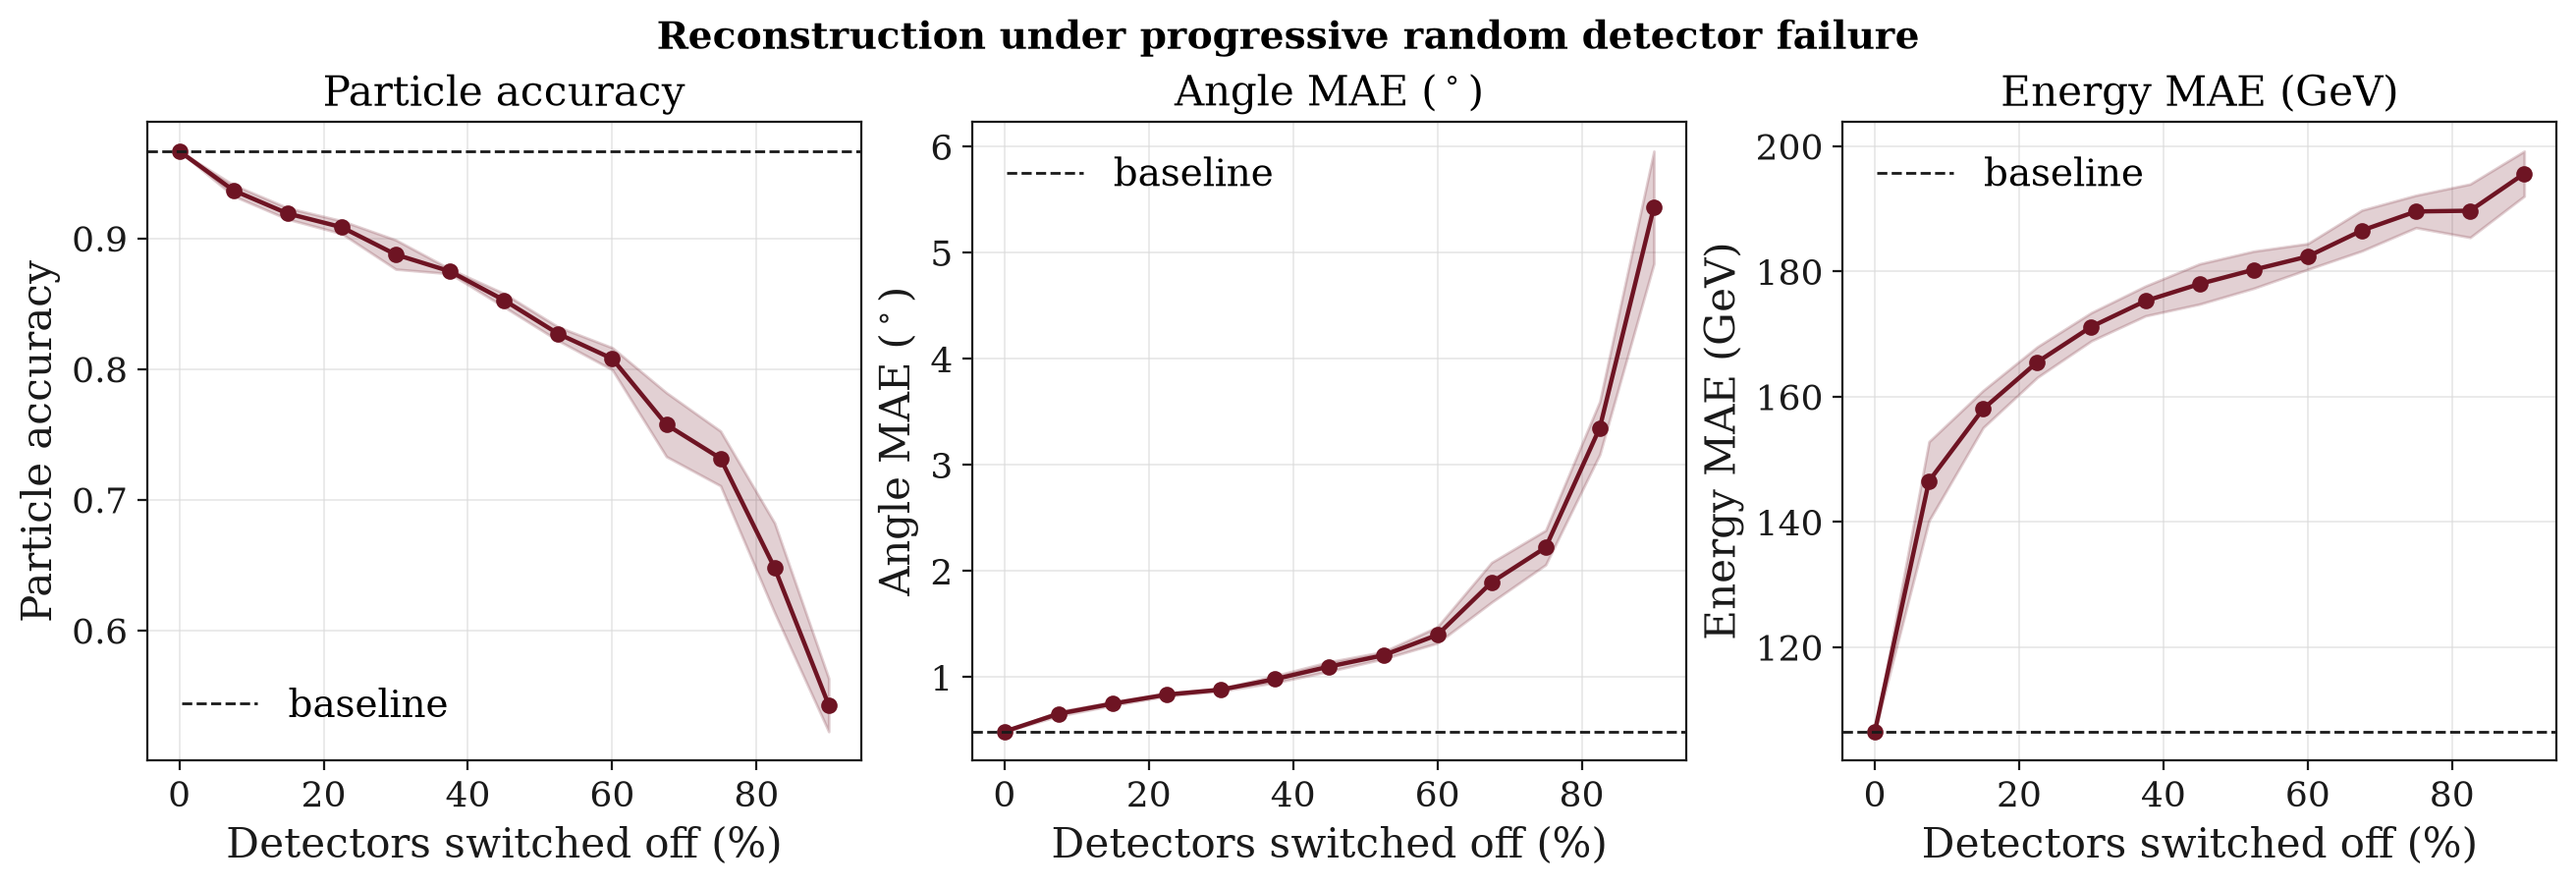
\includegraphics[width=1\linewidth]{figures/dropout_progressive.png}
    \caption[Reconstruction under progressive random detector failure.]{Task metric as a function of the fraction of detectors switched off at random. Shaded bands indicate one standard deviation over four random subsets per fraction. Dashed horizontal lines indicate baseline performance with all detectors active.}
    \label{fig:dropout_progressive}
\end{figure*}

Gamma-hadron classification is the most fault-tolerant task: accuracy stays above $90\%$ with up to about $22\%$ of the detectors offline and above $85\%$ up to roughly $45\%$, collapsing more steeply only beyond ${\sim}60\%$ loss.

The angular and energy reconstruction tasks begin to degrade more immediately. Angular MAE grows steadily, roughly doubling from its $0.49\degree$ baseline to ${\sim}1.0\degree$ at about $45\%$ detector loss and rising sharply thereafter. Energy MAE increases quickly at first --- from $107$~GeV to ${\sim}171$~GeV by $30\%$ loss --- and then saturates near $185$--$195$~GeV, a plateau that reflects the model falling back toward predicting the mean energy of the range once too few detectors survive to constrain the shower size.

This difference in fault tolerance reflects the nature of each task: binary classification can exploit redundant evidence across many detectors and remains viable as long as some discriminative detectors survive, while metric regression requires information from a spatially distributed set of detectors to triangulate the shower geometry and measure its total energy. The knee in the particle-accuracy curve near $60$--$70\%$ corresponds to the point at which too few spatially distinct measurements survive to resolve the shower footprint.

\textbf{Layout at matched detector count.} Random thinning reduces the detector count while leaving the covered area unchanged, so it does not separate the effect of the number of detectors from that of their arrangement. Figure~\ref{fig:dropout_geometry} compares three ways of reaching the same count: random thinning (detectors removed uniformly at random, sparser over the same area), central crop (only detectors within a shrinking radius are retained, denser over a smaller area), and a checkerboard pattern (every other detector removed, approximately halving the count while maintaining full coverage). At equal detector count, the differences between the three curves are attributable to the arrangement alone.

\begin{figure*}[ht!]
    \centering
    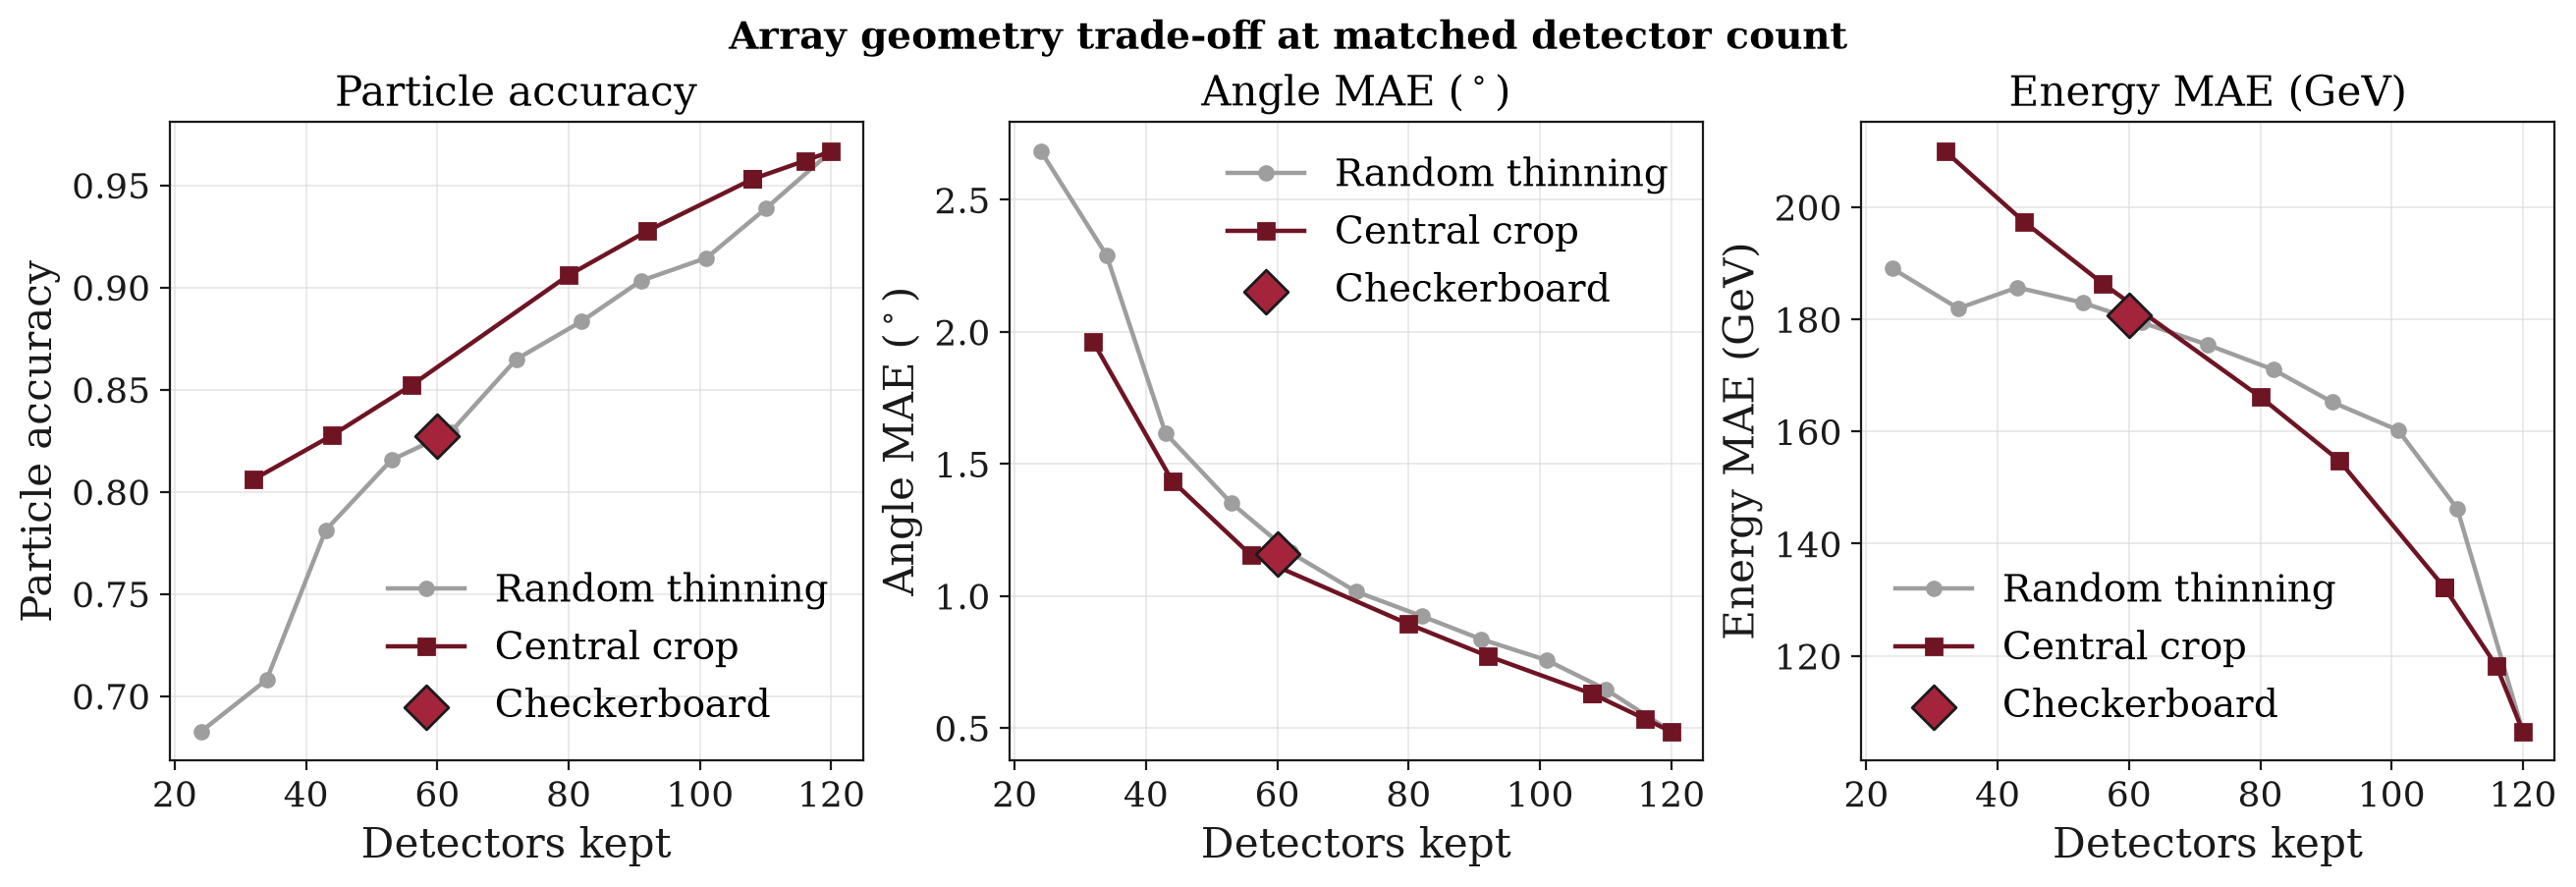
\includegraphics[width=1\linewidth]{figures/dropout_geometry.png}
    \caption[Array geometry trade-off at matched detector counts.]{Reconstruction performance as a function of the number of active detectors, for three sparsification strategies. Central crop (denser, smaller array) outperforms random thinning (sparser, same area) at equal detector count for classification and angular reconstruction; for energy the central crop wins only above ${\sim}65$ detectors and random thinning is better below that. The checkerboard point (diamond) corresponds to approximately 60 active detectors.}
    \label{fig:dropout_geometry}
\end{figure*}

The central crop strategy outperforms random thinning at matched detector counts for gamma-hadron classification and angular reconstruction at every count tested: for these two tasks, retaining the detectors closest to the array centre yields better reconstruction than retaining a random subset distributed over the full array area. Energy reconstruction, however, behaves differently. At high detector counts the central crop still performs better, but below roughly 65 active detectors the ordering reverses and random thinning gives the lower energy MAE. This crossover is consistent with the per-detector result of Section~\ref{subsec:regional}, where the peripheral modules were found to be nearly as valuable per unit as the core modules for energy: energy estimation relies on sampling the lateral extent of the shower, so under aggressive thinning a wide but sparse layout preserves outer footprint information that a dense central cluster discards. The checkerboard pattern (about 60 active detectors) falls close to the random-thinning curve for all three tasks, and in particular sits near this energy crossover, performing comparably to random thinning while remaining inferior to the central crop for classification and angular reconstruction.

Taken across the three studies, the results point in a consistent direction. Classification and angular reconstruction degrade least under the central crop, favouring a denser core; energy reconstruction follows the lateral spread of the modules instead and, below roughly 65 active detectors, favours a wide sparse layout over a dense central cluster. A dedicated study of the array layout, including geometries outside the present family such as hexagonal grids, variable pitch, or elliptical footprints, would re-run the CORSIKA pipeline and retrain the model for each configuration, and is left for future work.
    
    % Chapter 5: Conclusions %
    \chapter{Conclusions}
\label{ch:conclusions}

This thesis developed and evaluated a multi-task CNN-Transformer model for the simultaneous reconstruction of three EAS properties at CONDOR --- gamma-hadron classification, zenith angle, and primary energy --- on CORSIKA-simulated events in the 300--800 GeV range. The architecture extends the three-stream design of~\shortciteA{navarro2026transformer} to six independent Transformer streams, two per task, one over the CNN-processed sequence and one over the raw hit sequence, which makes attention available at the level of individual detector hits.

% ============================================================
\section{Summary of Contributions}
\label{sec:contributions}
% ============================================================

\textbf{A multi-task CNN-Transformer model for EAS reconstruction.} The central contribution is the reconstruction model itself: a single network that recovers particle type, zenith angle, and primary energy in one pass over the detector hits, with a shared convolutional backbone feeding task-specific Transformer streams. It extends the published three-stream design of~\shortciteA{navarro2026transformer} to six streams, adding one attention stream per task that operates directly on the raw hit sequence, so that the weighting each task learns can be examined at the level of individual hits.

\textbf{Multi-task reconstruction in the sub-TeV regime.} The model reaches AUC = 0.991 ($Q$-factor 5.48) for gamma-hadron discrimination, angular MAE = $0.484\degree$ (PSF$_{68} = 0.50\degree$), and energy MAE = 103.72 GeV. The angular resolution improves upon~\shortciteA{navarro2025multi} by a factor of 2.4 and lies well below the $1\degree$ threshold relevant for point-source identification. To the best of our knowledge, this is the only published work addressing the three EAS reconstruction tasks simultaneously at this altitude and energy range with an integrated explainability framework.

\textbf{Performance by energy and zenith angle.} Gamma-hadron discrimination degrades with energy in a physically consistent way (AUC from 0.998 at 300 GeV to 0.981 at 800 GeV) and is stable across the full zenith range (AUC 0.984--0.994).

\textbf{Physically consistent explainability.} Feature ablation and PFI agree on what each task uses: zenith reconstruction is dominated by temporal information by a wide margin (ablation: $+12.4\degree$ of added MAE), consistent with the arrival-time gradient as the primary geometric handle for direction; gamma-hadron discrimination relies on energy deposition and spatial features; and energy estimation is governed by spatial position, consistent with the correlation between lateral extent and primary energy.

\textbf{RAW attention streams and hit-level interpretability.} The RAW Transformer streams produce attention matrices directly over the individual hit sequence, so the weighting learned by each task can be examined at the level of detector hits rather than of CNN features. The three streams learn distinct distributions: classification concentrates $82\%$ of its weight on the first ten hits, angle reconstruction assigns $80\%$ to hits later than the query and peaks near the end of the sequence, and energy estimation lies between the two, in agreement with the feature importance results.

\textbf{Robustness to missing detectors.} The detector dropout analysis characterises how
the trained reconstruction model responds to missing detector information, measured by
switching detectors off at inference without retraining. Gamma-hadron classification is the most fault-tolerant task, holding accuracy above $90\%$ with up to approximately $22\%$ of modules offline, while angular and energy reconstruction degrade sooner. Removing the central core is the most damaging block-level failure for classification, whereas angular reconstruction depends at least as much on the surrounding modules, which sample the lateral extent over which the arrival-time gradient is measured; and per module removed, the 20 peripheral units cost almost as much for energy as the central ones, so they are not redundant despite ranking last as a block. Because the model was trained only on the full array, these figures bound the degradation from above and indicate where the reconstruction relies on the array, rather than prescribing how many detectors to build or how to place them.

% ============================================================
\section{Limitations and Future Work}
\label{sec:limitations}
\label{sec:future}
% ============================================================

The limitations of this work and the lines of research that would address them are presented together, since most of the former define the latter.

\textbf{Simulation-only evaluation.} All results are obtained on CORSIKA-simulated events; CONDOR is a proposed observatory with no measured data yet, so generalization to real detector behaviour, with hardware noise, gain variations, detector aging, and atmospheric conditions not captured by CORSIKA, cannot be assessed here. Once the observatory begins scientific operations the model can be applied to measured events, a transition that will likely require domain adaptation, data-driven calibration of the normalization statistics, and fine-tuning on hybrid simulation-data samples.

\textbf{Energy coverage.} The dataset comprises three discrete energy points (300, 500, and 800 GeV), sufficient to demonstrate multi-task learning in a controlled setting but not representative of the continuous cosmic ray spectrum; the regression-toward-the-mean bias is a direct consequence of that discretization. Performance below 300 GeV, approaching the CONDOR threshold, and above 1 TeV is likewise not characterized. Sampling the energy from a power law would remove the bias and model the flux realistically, at the cost of new CORSIKA simulations and a re-run of the preprocessing pipeline.

\textbf{Fixed azimuthal angle.} All simulated showers use a fixed azimuthal angle of $\phi = 0\degree$. The array geometry gives this simplification little support: in the proposed layout, both the modules and the central grid they form are rectangular rather than square in their two horizontal dimensions, so the array is invariant only under a $180\degree$ rotation, and the choice introduces directional biases in the learned attention patterns and in the regional dropout results (Sections~\ref{subsec:attention} and~\ref{subsec:regional}). Because the core also lands at a different position in each event, $\phi$ cannot be obtained by a geometric transformation of the $\phi = 0\degree$ model and must be learned from a dataset with uniformly sampled azimuth, possibly with positional embeddings that encode detector coordinates explicitly.

\textbf{Attention as an explainability method.} The attention maps describe how each stream weights its input sequence, but they do not attribute the prediction to those inputs, and two properties of the mechanism limit what can be read from them. The weights of each row are normalized over the valid hits of the event, so their scale depends on the number of active modules, which itself differs systematically between gamma and proton showers; comparisons between classes are therefore not directly interpretable as differences in model behaviour. And a map estimated from a finite sample carries structure of its own, which a map shown without an associated uncertainty does not reveal. The analysis is accordingly restricted to the aggregate distribution of the weights per task, and the feature-level conclusions rest on the intervention-based methods of Section~\ref{sec:explainability}.

\textbf{Single training run.} All results come from a single training run with a fixed random seed, so the variability of the metrics across initializations is not characterized. The narrow train-validation gap and the consistency across groups suggest the results are not an artifact of a particular seed, but confidence intervals from independent runs would be stronger evidence.

\textbf{Multi-task advantage not quantified.} The three tasks are optimized jointly under the premise that shared representations benefit physically correlated objectives, but the model was not benchmarked against three independently trained single-task networks, so that advantage is not established here. Training single-task variants, removing the RAW or CNN streams, and varying the number of attention heads would isolate the contribution of each component and settle the question.

\textbf{Single observatory.} The model is tailored to the CONDOR array geometry; the input representation, the normalization statistics, and the learned representations are specific to it, and transfer elsewhere would require retraining. Adapting the framework to instruments such as HAWC, LHAASO, or the future SWGO, which cover complementary energy ranges at different altitudes and geometries, is a natural path toward cross-experiment consistency.

\textbf{Uncertainty quantification.} The model produces point estimates. Bayesian layers, Monte Carlo dropout at inference, or normalizing flows on the output distributions would provide event-by-event confidence intervals, useful for downstream analyses such as source detection and spectral unfolding; this direction is being explored in a related effort applying Bayesian neural networks to the CONDOR reconstruction problem.

\textbf{Array geometry.} Finally, the robustness results motivate evaluating alternative layouts: hexagonal grids, elliptical footprints, and variable-pitch designs could improve reconstruction for a fixed hardware budget. Any such study requires re-running the CORSIKA pipeline on the new detector positions, since the processed dataset encodes the current geometry at the level of individual hit aggregations.

    % References %
    \cleardoublepage
    % \addcontentsline{toc}{chapter}{References}
    \renewcommand{\bibliographytypesize}{\small}
    \begingroup
    \setlength{\itemsep}{0.3ex plus 0.1ex}
    \bibliography{references}
    \endgroup
    
    % Appendix %
    \appendix 

\chapter{Supplementary Material} \label{ch:appendix}

\section{Atmospheric Depth} \label{sec:apx_depth}

The development of an air shower is described as a function of \textit{atmospheric depth} rather than of altitude or of distance travelled, and quantities such as $X_{\text{max}}$ are consequently reported in $\mathrm{g \ cm}^{-2}$. This section sets out why that variable is the natural one and what the choice implies for the two aspects of this work that depend on it: the reconstruction of the zenith angle and the altitude of the observation site.

The atmosphere is the target in which the cascade develops, and its density falls by orders of magnitude between the top of the atmosphere and the ground. The vertical atmospheric depth at an altitude $h$ is defined as the integral of the air density above that altitude,
\begin{equation}
    X_v(h) = \int_h^{\infty} \rho(h') \, \mathrm{d}h' \ ,
    \label{eq:atmospheric_depth}
\end{equation}
that is, the mass of air per unit area contained in the column above the point in question, which is where the units come from. Because the atmosphere is in hydrostatic equilibrium, this column mass is exactly what a barometer measures: $X_v = P/g$, with $P$ the local pressure and $g$ the gravitational acceleration. The vertical depth at sea level, close to $1{,}030 \ \mathrm{g \ cm}^{-2}$, is standard atmospheric pressure written as a mass column.

The reason this quantity, and not the geometric path length, is the coordinate of shower development is that the probability of an interaction depends on the amount of matter traversed. Consider a particle crossing a layer of thickness $\mathrm{d}l$ in air of density $\rho$, with a cross-section $\sigma$ per target nucleus of mass number $A$. The number density of targets is $n = \rho N_A / A$, so the interaction probability over the layer is $n \sigma \, \mathrm{d}l = (N_A \sigma / A) \, \rho \, \mathrm{d}l$. The density and the geometric length appear only through the product $\rho \, \mathrm{d}l \equiv \mathrm{d}X$, so the survival probability after traversing a depth $X$ is
\begin{equation}
    P_{\text{surv}}(X) = \exp\left(-X / \lambda\right) \ , \qquad \lambda = \frac{A}{N_A \sigma} \ ,
    \label{eq:interaction_length}
\end{equation}
where the interaction length $\lambda$ is itself expressed in $\mathrm{g \ cm}^{-2}$. The same argument holds for radiative processes, whose characteristic scale is the radiation length, $X_0 \approx 36.6 \ \mathrm{g \ cm}^{-2}$ in air~\shortcite{ParticleDataGroup2024}. A particle does not respond to how far it has moved but to how much matter it has crossed, and depth is the variable that counts the latter. Expressing the atmosphere in metres would require carrying the altitude dependence of $\rho$ through every step of the calculation; expressing it in $\mathrm{g \ cm}^{-2}$ absorbs that dependence once and for all.

A direct consequence is that the longitudinal profile of a shower is, to a good approximation, a universal function of $X$. Two showers of the same primary energy whose first interactions occur at different altitudes pass through the same sequence of generations, and their profiles coincide when expressed in depth even though they do not coincide when expressed in metres. This is why the Heitler model of Section~\ref{subsec:electromagnetic_showers} yields a depth of maximum, Equation~\ref{eq:xmax}, rather than a height of maximum, and why $X_{\text{max}}$ is comparable across showers, experiments, and sites.

Expressed in these terms, the atmosphere is a calorimeter whose thickness is measured in radiation lengths: the vertical column at sea level amounts to $1{,}030 / 36.6 \approx 28 \, X_0$, and less at altitude. That thickness is not a fixed property of the instrument but is set jointly by the observation level and by the arrival direction of each individual shower, which is the sense in which a ground-based array measures every cascade at whatever stage of development it happens to have reached on arrival.

A shower arriving at a zenith angle $\theta$ does not traverse the vertical column but the column along its own axis, known as the slant depth. For a plane-parallel atmosphere, the approximation adopted in CORSIKA~\shortcite{Heck1998}, the two are related by
\begin{equation}
    X(\theta) = X_v \sec\theta \ .
    \label{eq:slant_depth}
\end{equation}
An inclined shower therefore crosses more matter before reaching the array than a vertical shower of the same energy: about 6\% more at $\theta = 20\degree$ and about 30\% more at $\theta = 40\degree$, the upper limit of the range simulated in this work. The approximation is accurate over that range and degrades only for nearly horizontal showers, where the curvature of the Earth can no longer be neglected. The physical consequence is that the zenith angle and the effective observation depth are two views of the same variable: a shower observed at larger $\theta$ is observed at a later stage of its development, with fewer surviving particles and a wider, more attenuated footprint. That systematic is what the angular reconstruction task exploits, and it is visible directly in the evolution of the mean footprint with $\theta$ shown in Figure~\ref{fig:angle_evolution}.

The same relation accounts for the value of altitude in the design of a ground-based array. Table~\ref{tab:atmospheric_depths} lists the vertical depth at several observation levels. Placing the array at 5,300 m removes roughly half of the atmospheric column that a detector at sea level must look through, and about 90 $\mathrm{g \ cm}^{-2}$ relative to HAWC. Since the number of particles surviving to ground falls steeply with the depth traversed beyond the shower maximum, and sub-TeV showers reach their maximum high in the atmosphere, that difference translates into a substantially larger number of secondaries at ground level for a primary of a given energy. This is the origin of the low energy threshold discussed in Section~\ref{sec:condor_observatory}, and it is a property of the site rather than of the detector technology.

\begin{center}
\begin{minipage}{\linewidth}
\centering
\captionof{table}[Vertical atmospheric depth at several observation levels.]{Vertical atmospheric depth at several observation levels, computed from the U.S.\ standard atmosphere. Values are rounded to the nearest $5 \ \mathrm{g \ cm}^{-2}$.}
\label{tab:atmospheric_depths}
\setlength{\tabcolsep}{8pt}
\renewcommand{\arraystretch}{1.2}
\begin{tabular}{llr}
\toprule
\textbf{Observation level} & \textbf{Altitude} & \textbf{Vertical depth} \\
\midrule
Sea level & 0 m & $1{,}030 \ \mathrm{g \ cm}^{-2}$ \\
HAWC & 4,100 m & $620 \ \mathrm{g \ cm}^{-2}$ \\
LHAASO & 4,410 m & $595 \ \mathrm{g \ cm}^{-2}$ \\
CONDOR & 5,300 m & $530 \ \mathrm{g \ cm}^{-2}$ \\
\bottomrule
\end{tabular}
\end{minipage}
\end{center}

\section{Model Architecture Summary} \label{sec:apx_architecture}

Table~\ref{tab:model_layers} provides a layer-by-layer breakdown of the CNN-Transformer multi-task model and its parameter counts, grouped by functional block. Each Transformer stream is a pre-norm encoder block; the CNN streams operate on the 128-dimensional backbone output and the RAW streams on the six-dimensional masked hit sequence, which is why the former account for roughly twenty times the parameters of the latter. All counts are read directly from the trained model.

\begin{center}
\begin{minipage}{\linewidth}
\centering
\captionof{table}[Layer-by-layer model summary.]{Layer-by-layer summary of the CNN-Transformer model, with parameter counts grouped by functional block.}
\label{tab:model_layers}
\small
\setlength{\tabcolsep}{6pt}
\renewcommand{\arraystretch}{1.05}
\begin{tabular}{llr}
\toprule
\textbf{Component} & \textbf{Layer} & \textbf{Parameters} \\
\midrule
\multirow{7}{*}{CNN backbone}
  & Conv1D (128 filters, $k$=7) + BN + ELU & 6,016 \\
  & Conv1D (128 filters, $k$=7) + BN + ELU & 115,328 \\
  & Conv1D (128 filters, $k$=7) + BN + ELU & 115,328 \\
  & MaxPool1D (stride=2) & 0 \\
  & Dense(128) + ELU & 16,512 \\
  & Dense(256) + ELU + Dropout(0.4) & 33,024 \\
  & Dense(128) + ELU & 32,896 \\
\midrule
\multirow{2}{*}{Transformer $\times$ 6}
  & 3 CNN streams (LN + MHA + FFN) & 150,432 \\
  & 3 RAW streams (LN + MHA + FFN) & 7,692 \\
\midrule
\multirow{3}{*}{Output heads}
  & Classification: Dense(128) + Dense(1, sigmoid) & 18,049 \\
  & Angle: Dense(128) + Dense(1, linear) & 18,049 \\
  & Energy: Dense(128) + Dense(1, linear) & 18,049 \\
\midrule
\multicolumn{2}{l}{\textbf{Total parameters}} & \textbf{531,375} \\
\multicolumn{2}{l}{\quad Trainable} & 530,607 \\
\multicolumn{2}{l}{\quad Non-trainable (BN statistics)} & 768 \\
\bottomrule
\end{tabular}
\end{minipage}
\end{center}

\section{Global Feature Definitions} \label{sec:apx_global_features}

Table~\ref{tab:global_features_order} specifies the exact computation and ordering of the five global features as implemented in the preprocessing pipeline.

\begin{center}
\begin{minipage}{\linewidth}
\centering
\captionof{table}[Global feature computation and ordering.]{Global feature vector: computation, ordering, and normalization as implemented in the code.}
\label{tab:global_features_order}
\setlength{\tabcolsep}{5pt}
\renewcommand{\arraystretch}{1.2}
\begin{tabular}{clll}
\toprule
\textbf{Index} & \textbf{Name} & \textbf{Computation} & \textbf{Normalization} \\
\midrule
0 & \texttt{total\_particles}   & $\sum_i \texttt{count}_i$ & Min-max \\
1 & \texttt{total\_energy}      & $\sum_i \varepsilon_i$ & Min-max \\
2 & \texttt{active\_detectors}  & Number of unique detector IDs & Min-max \\
3 & \texttt{duration}           & $t_\text{max} - t_\text{min}$ & Min-max \\
4 & \texttt{central\_energy}    & $\sum_{i \in \mathcal{C}} \varepsilon_i$ & Min-max \\
\bottomrule
\multicolumn{4}{l}{\footnotesize $\mathcal{C}$: set of 16 central detector modules closest to the array origin.}
\end{tabular}
\end{minipage}
\end{center}

\section{Quality Factor Definition} \label{sec:apx_qfactor}

The quality factor $Q$ is a standard figure of merit in gamma-ray astronomy that quantifies the signal-to-noise improvement achieved by a classifier. For a given classification threshold, the gamma-ray efficiency $\varepsilon_\gamma$ is the fraction of true gamma events correctly classified, and the proton survival rate $\varepsilon_p$ is the fraction of proton events misclassified as gamma. The quality factor is defined as
\begin{equation}
    Q = \frac{\varepsilon_\gamma}{\sqrt{\varepsilon_p}} \ .
\end{equation}
A larger $Q$ indicates a better signal-to-noise ratio after classification. For the model presented in this thesis, at the default threshold of $P(\gamma) = 0.5$, the quality factor evaluates to $Q = 5.48$ with $\varepsilon_\gamma = 0.971$.

\section{Angular Resolution: PSF\texorpdfstring{$_{68}$}{68} Definition} \label{sec:apx_psf}

The angular resolution of a ground-based gamma-ray observatory is conventionally reported as a containment radius rather than as a mean error. The reason is that the distribution of angular residuals is not Gaussian: it is asymmetric and carries a tail of poorly reconstructed events, produced by showers whose core falls near the edge of the array or whose front is sampled by few detectors, which would dominate a mean-based figure of merit while affecting only a small fraction of the data. Characterizing the resolution through the shape of the residual distribution rather than through a single moment is long-established practice for scintillator arrays~\shortcite{prahl1993procedure}, and containment radii are the form in which contemporary ground-based arrays such as HAWC report their angular performance~\shortcite{HAWK}.

For each test event, the \textit{angular residual} is the difference between the reconstructed and true zenith angles, $\hat{\theta} - \theta_\text{true}$, and the absolute angular error is $\Delta\theta = |\hat{\theta} - \theta_\text{true}|$. The point spread function at 68\% containment, PSF$_{68}$, is the 68th percentile of the distribution of $\Delta\theta$ over the test set:
\begin{equation}
    \text{PSF}_{68} = \inf \left\{ r \geq 0 \ : \ P\left( \Delta\theta \leq r \right) \geq 0.68 \right\} \ .
\end{equation}
In words, PSF$_{68}$ is the angular radius around the true direction within which 68\% of reconstructed events fall. The 68\% level is chosen because it corresponds to the fraction of a one-dimensional Gaussian distribution contained within one standard deviation, which makes the quantity directly comparable to a resolution quoted as $\sigma$ for instruments whose residuals happen to be Gaussian, without assuming that they are. For the model presented in this thesis, PSF$_{68} = 0.50\degree$.

\begin{quote}
\textbf{Scope of this definition.} An observatory normally quotes PSF$_{68}$ over the \textit{space angle} $\psi$, which combines the zenith and azimuth residuals into a single separation on the sky. Here the azimuth is fixed at $\phi = 0\degree$ (Section~\ref{sec:corsika}) and is not reconstructed, so the value above is a zenith-only containment radius: a lower bound on the space-angle PSF$_{68}$ that the same architecture would reach with the azimuth left free. Comparisons with observatories that reconstruct both angles should be read with that restriction in mind.
\end{quote}


\end{document}